%
%reference: http://texwelt.de/wissen/fragen/3772/wie-gehe-ich-eine-bachelorarbeit-mit-latex-an
%

\documentclass[twoside]{scrartcl}


\usepackage[utf8]{inputenc}
%\usepackage{geometry}
\usepackage{fixme}
\usepackage{csquotes}
\usepackage{mdframed}
\usepackage{tensor}
\usepackage{amsthm}
\usepackage{amsmath}
\usepackage{mathtools}
\usepackage{amsfonts}
\usepackage{amssymb}
\usepackage{stmaryrd}
\usepackage{acro}
\usepackage{stmaryrd}
\usepackage{url}
\usepackage{tikz}
\usepackage{mathtools}
\usepackage{bussproofs}
\usepackage{syntax}
\usepackage[inline]{enumitem}
\usepackage[style=numeric,backend=bibtex]{biblatex}
\usepackage[final]{listings}
%\usepackage{hyperref}

\bibliography{bibliography}{}

\lstset{
	numbers=left,
	frame=lrtb,
	emph={while,fork,null,do,done,if,then,else,fi,skip,new,join},
	emphstyle=\textbf,
	mathescape
}

% -- tikz settings: --
\usetikzlibrary{arrows, cd, positioning, backgrounds, fit, decorations.pathmorphing, shapes.misc, calc}
\tikzset{%
	node/.style={draw, minimum size=8mm, inner sep=0mm, circle, fill=green!50},
	var/.style={draw, rectangle, minimum width=16mm, minimum height=6mm,%
		rounded corners=3pt, node distance=1cm, fill=purple!30},
	connector/.style={thick},
	sel/.style={->,thick},
	perm/.style={draw, rectangle},
	he/.style={draw, rectangle, minimum width=10mm, fill=blue!50},
	ext/.style={fill=brown!45},
	textnode/.style={draw, inner sep=4mm, rectangle, rounded corners=4pt}
}



%operator:
\newcommand*\circled[1]{\tikz[baseline=(char.base)]{
            \node[shape=circle,draw,inner sep=2pt] (char) {#1};}}

\newcommand{\Emb}{\mathit{Emb}}
\newcommand{\out}{\mathit{out}}
\newcommand{\fpHRG}{\mathit{fpHRG}_{\Sigma_{N}}^{\PI}}
\newcommand{\reach}{\mathit{reach}}
\newcommand{\FP}{\mathit{FP}}
\newcommand{\ap}{\mathit{ap}}
\newcommand{\fp}{\mathit{fp}}
\newcommand{\Proc}{\mathit{Proc}}
\newcommand{\emb}{\mathit{emb}}
\newcommand{\PI}{\mathit{Var}_{\text{process}}}
\newcommand{\rea}{\mathit{rea}}
\newcommand{\btr}{\blacktriangleright}
\newcommand{\type}{\mathit{type}}
\newcommand{\abs}{\mathit{abs}}
\newcommand{\br}{\mathit{br}}
\newcommand{\RB}{\mathit{RB}}
\newcommand{\NT}{\mathit{NT}}
\newcommand{\lhs}{\mathit{lhs}}
\newcommand{\rhs}{\mathit{rhs}}
\newcommand{\Tok}{\mathit{Tok}}
%\newcommand{\path}{\mathit{path}}
\newcommand{\Path}{\mathit{Path}}
\newcommand{\CPath}{\mathit{CPath}}
\newcommand{\AHC}{\mathit{AHC}_{\Sigma_{N}}^{\PI}}
\newcommand{\rk}{\mathit{rk}}
\newcommand{\con}{\mathit{con}}
\newcommand{\lab}{\mathit{lab}}
\newcommand{\ext}{\mathit{ext}}
\newcommand{\perm}{\mathit{perm}}
\newcommand{\HRG}{\mathit{HRG}_{\Sigma_{N}}^{\PI}}
\newcommand{\DSG}{\mathit{DSG}_{\Sigma_{N}}^{\PI}}
\newcommand{\HAG}{\mathit{HAG}_{\Sigma_{N}}^{\PI}}
\newcommand{\PES}{\mathit{PES}_{\PI}}
\newcommand{\HC}{\mathit{HC}_{\Sigma}^{\PI}}
\newcommand{\HCN}{\mathit{HC}_{\Sigma_{N}}^{\PI}}
\newcommand{\HG}{\mathit{HG}_{\Sigma}^{\PI}}
\newcommand{\HGN}{\mathit{HG}_{\Sigma_{N}}^{\PI}}
\newcommand{\aHG}{\mathit{HG}_{\Sigma_{N}}^{\PI}}
\newcommand{\HRule}{\rule{\linewidth}{0.5mm}}
\newcommand{\Sel}{\mathit{Sel}}
\newcommand{\Var}{\mathit{Var}}
\newcommand{\enum}{\mathit{enum}}
\newcommand{\Cont}{\mathit{Cont}}
\newcommand{\afiso}{\tensor[_\ap]{\cong}{_\fp}}
\newcommand{\border}{\mathit{border}}
\newcommand{\img}{\mathit{img}}
\newcommand{\off}{\mathit{offspring}}



%environments:
\newtheorem{defi}{Definition}[section]
\newtheorem{theorem}{Theorem}[section]
\newtheorem{lemma}{Lemma}[section]
\newtheorem{corollary}{Corollary}[section]
\newtheorem{claim}{Claim}[section]

\newenvironment{definition}
	{\begin{mdframed}[nobreak=true]\begin{defi}}
	{\end{defi}\end{mdframed}}

%acronyms:
\DeclareAcronym{HAG}{
	short = HAG,
	long  = Heap Abstraction Grammar
}
\DeclareAcronym{AHC}{
	short = AHC,
	long  = admissible heap configuration
}
\DeclareAcronym{DSG}{
	short = DSG,
	long  = data structure grammar
}
\DeclareAcronym{HG}{
	short = HG,
	long  = hypergraph
}

\DeclareAcronym{HC}{
	short = HC,
	long  = heap configuration
}

\DeclareAcronym{HRG}{
	short = HRG,
	long  = hyperedge replacement grammar
}

\DeclareAcronym{fpHRG}{
	short = fpHRG,
	long  = fully permissive HRG
}

\DeclareAcronym{HR}{
	short = HR,
	long  = hyperedge replacement
}

\DeclareAcronym{PE}{
	short = PE,
	long  = permission expression
}

\DeclareAcronym{PES}{
	short = PES,
	long  = permission expression set
}

\DeclareAcronym{PM}{
	short = PM,
	long  = permission model
}

\DeclareAcronym{HM}{
	short = HM,
	long  = hypergraph morphismen
}

\begin{document}
\begin{titlepage}
\begin{center}
{\Large Rheinische-Westfälische Technische Hochschule Aachen\\
Lehrstuhl für Informatik 2\\
Software Modeling and Verification\\
Prof. Dr. Ir. Joost-Pieter Katoen}\\[1cm]
\today\\[1.5cm]
{\Large \textbf{Bachelor Thesis}}\\[1.5cm]
\HRule\\[0.8cm]
{\LARGE \textbf{Thread-Modular Analysis of Heap-Manipulating Programs}\\[0.2cm]}
\HRule\\[2cm]
\resizebox{!}{5.5cm}{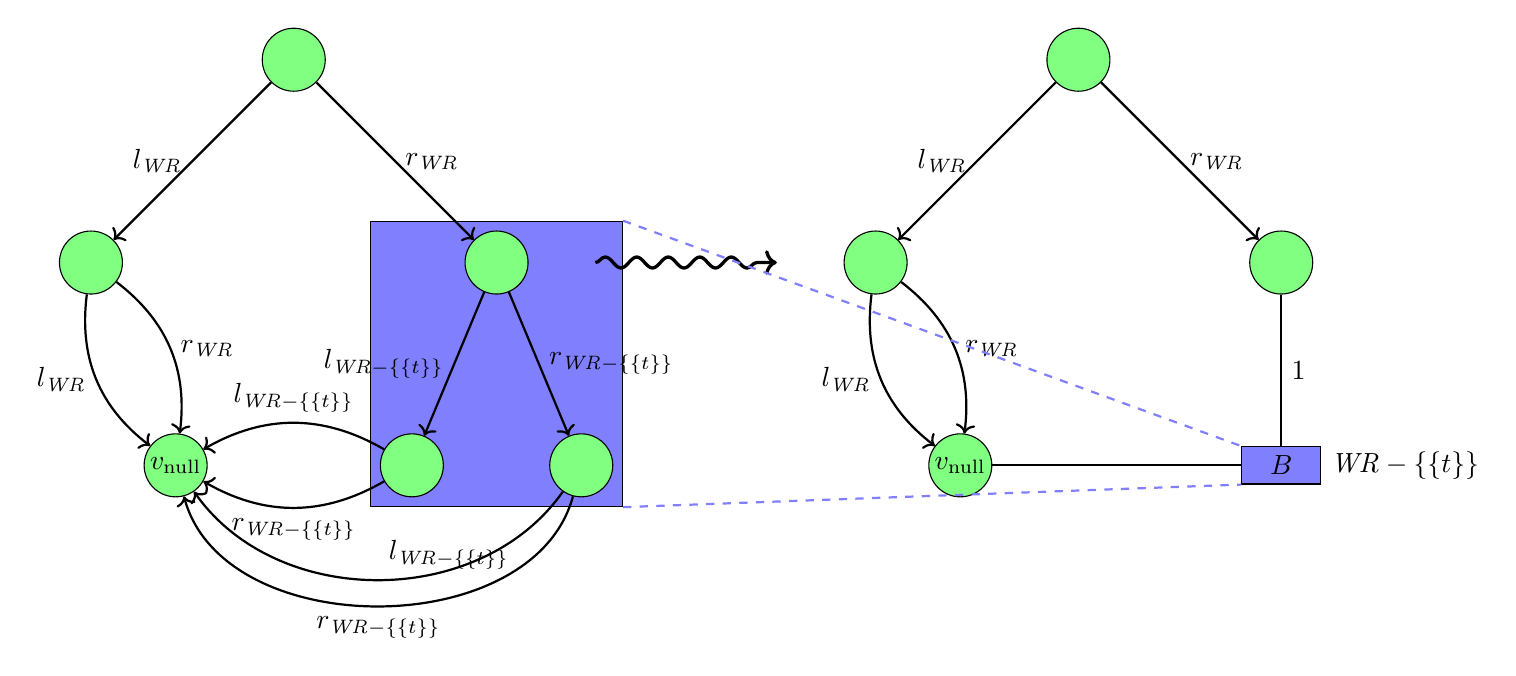
\begin{tikzpicture}[node distance=2 and 2]
	\node [node] (v1) {};
	\node [node, below left=of v1] (v2) {};
	\node [node, below right=of v1] (v3) {};
	\node [node, below left=2 and 0.5 of v3] (v4) {};
	\node [node, below right=2 and 0.5 of v3] (v5) {};
	\node [node, right =4 of v3] (v6) {};
	\node [node, above right=of v6] (v7) {};
	\node [node, below right=of v7] (v8) {};
	\node [node, below right= 2 and 0.5 of v2] (null1) {$v_{\text{null}}$};
	\node [node, below right= 2 and 0.5 of v6] (null2) {$v_{\text{null}}$};
	\node [he, label={0:$\mathit{WR}-\{\{t\}\}$}] (b) at (null2-|v8) {$B$};

	%left
	\draw [sel] (v1) to node[left]{$l_{\mathit{WR}}$} (v2);
	\draw [sel] (v1) to node[right]{$r_{\mathit{WR}}$} (v3);
	\draw [sel, bend right] (v2) to node[left]{$l_{\mathit{WR}}$} (null1);
	\draw [sel, bend left] (v2) to node[right]{$r_{\mathit{WR}}$} (null1);
	\draw [sel] (v3) to node[left]{$l_{\mathit{WR}-\{\{t\}\}}$} (v4);
	\draw [sel] (v3) to node[right]{$r_{\mathit{WR}-\{\{t\}\}}$} (v5);
	\draw [sel, bend right] (v4) to node[above]{$l_{\mathit{WR}-\{\{t\}\}}$} (null1);
	\draw [sel, bend left] (v4) to node[below]{$r_{\mathit{WR}-\{\{t\}\}}$} (null1);
	\draw [sel, bend left=55] (v5) to node[above right]{$l_{\mathit{WR}-\{\{t\}\}}$} (null1);
	\draw [sel, bend left=75] (v5) to node[below]{$r_{\mathit{WR}-\{\{t\}\}}$} (null1);

	%right
	\draw [sel] (v7) to node[left]{$l_{\mathit{WR}}$} (v6);
	\draw [sel] (v7) to node[right]{$r_{\mathit{WR}}$} (v8);
	\draw [sel, bend right] (v6) to node[left]{$l_{\mathit{WR}}$} (null2);
	\draw [sel, bend left] (v6) to node[right]{$r_{\mathit{WR}}$} (null2);
	\draw [connector] (b) to node[right]{$1$} (v8);
	\draw [connector] (b) to (null2);

	\node [right=0.6 and 0.6 of v3] (d1) {};
	\node [left=0.6 and 0.6 of v6] (d2) {};

	\draw [very thick,->, decorate,
	decoration={snake,amplitude=.7mm, segment length=4mm, post length=2mm}] (d1) to (d2);

	\begin{scope}[on background layer]
		\node [he, fit=(v3) (v4) (v5)] (layer) {};
	\end{scope}

	\draw [-, dashed, thick, color=blue!50] (layer.north east) to (b.north west); 
	\draw [-, dashed, thick, color=blue!50] (layer.south east) to (b.south west); 
\end{tikzpicture}
}
\end{center}
\vfill
\begin{tabular}{p{4cm}l}
Author: & Christoph Welzel\\
&\\
First Reviewer: & apl. Prof. Dr. Thomas Noll\\
Second Reviewer: & Prof. Dr. Ir. Joost Pieter Katoen\\
Advisor: & Christina Jansen\\
\end{tabular}

\end{titlepage}

\cleardoublepage
\pagestyle{empty}
\begin{abstract}
	\section*{Abstract}
	This paper presents a graph-based modelling of the structure of
	concurrent heap manipulating programs. It introduces a programming
	language that allows parallel execution in the means of fork and join.
	The semantics of the programming language is presented in terms of
	hypergraphs transformations. The main results are the abstraction of the
	heap structure by hyperedge replacement grammars
	which is proven to be a correct overapproximation
	and that the presented analysis can prove data race free executions of
	programs.
\end{abstract}
\vfill
\section*{Selbstständigkeitserklärung}
Hiermit versichere ich, dass ich die vorliegende Arbeit eigenständig
angefertigt habe und keine anderen Quellen oder Hilfsmittel als die angegebenen
benutzt habe. Alle wörtlichen oder sinngemäßen Zitate sind als solche
kenntlich gemacht.\\[4cm]
\begin{minipage}{0.5\textwidth}
	\makebox[1.5in]{\hrulefill}\\
	{\small(Christoph Welzel)}
\end{minipage}%
\begin{minipage}{0.5\textwidth}
	\begin{flushright}
		Aachen, den 15. August 2015
	\end{flushright}
\end{minipage}

\newpage
\cleardoublepage
\tableofcontents
\newpage
\pagestyle{plain}
\pagenumbering{arabic}
\setcounter{page}{2}
\section{Introduction}
\label{sec:introduction}
	Nowadays, software relies on the use of pointers. In order to make use of
	unbounded data structures these are modelled within the dynamically
	allocateable part of the memory, the \emph{heap}. As previous research has
	shown it is a viable approach to analyse pointer programs by representing
	the structure of the heap as \emph{hypergraph} \cites{InformalGraphGrammars}
	{InductivePredicates}{ProcedureSummaries}. This analysis focuses on
	different problems in the use of pointer in software, most notably the
	dereferencation of null pointers and memory leaks
	\cites{InformalGraphGrammars}{fmsd}.  Furthermore in order to obtain a
	finite representation of the unbounded data structures \emph{hyperedge
	replacement grammars} are used for abstraction.
	Those hyperedge replacement grammars allow to represent parts of the heap
	that can grow unboundedly in a finite manner but also to concretise
	abstracted parts on demand. This modelling technique is
	already used as basis for computational analysis by the tool Juggrnaut
	\cite{fmsd}. By now these techniques operate mainly on sequential execution
	of programs. Another possible approach on analysing pointer programs which
	relies on formulating structural properties of the heap in logical formulae
	is \emph{separation logic} \cite{PrimerSeparationLogic}. Because in
	separation logic the heap is
	separated in different parts which are reasoned about individually this
	approach has proven well suited for analysis of concurrent programs
	\cites{SeparationLogic}{AbstractSeparationLogic}{LocalReasoning}. This work
	is a contribution in widening the analysis technique of a graph-based
	representation to parallel executing programs. By approaching parallelism
	new challenges arise, most importantly \emph{data races}. Data races are
	situations where multiple processes access data at the same time and the
	result of these actions depend on each other. If data races occur all
	possible interleavings of the executions have to be examined which causes
	the possible states that have to be analysed to grow uncontrollably large.
	This is often
	referred to as \emph{state space explosion} e.g. in \cite[pp. 77-80]
	{PrinciplesOfModelChecking}. In order to avoid state space explosion it is
	possible to prove the absence of data races which resolves the dependency of
	the actions and allows to reduce the number of states that have to be
	examined. In separation logic this is approached by incorporating permission
	accounting into the formulae that describe the heap states. This permission
	accounting is a way to distinguish read and write access and can be used to
	prove data race freedom. As suggested e.g. in \cite{InductivePredicates} and
	\cite{ProcedureSummaries} this approach can be examined for graph-based
	representation of the heap. This is the  main contribution of this paper:
	incorporating permissions into the hypergraphs that are used to model the
	state of the heap and introducing a mechanism of parallelism by adding
	fork and join statements to the examined programming language. Where fork
	starts new processes and join
	synchronises other processes by waiting for their termination. This is
	explored in \cite{MultithreadedJavaPrograms} with some formal effort. The
	goal of the presented analysis is among other things to provide a more
	intuitive approach by graph-based representation of the heap. For the fork
	and join statemant appropiate semantics in the sense of graph
	transformations are defined. Central results of this work are the proof that
	the used abstraction via hyperedge replacement grammars support the
	incorporation of permissions and that the analysed states ensure data race
	freedom. For this result it is generally assumed that the behaviour of
	forked processes is determined by given contracts, similar to those that are
	automatically generated in \cite{ProcedureSummaries}.

\newpage
\section{Preliminaries}
	For a set $S$, $S^{*}$ are all finite sequences of elements from $S$.
	For such a sequence $s\in S^{*}$ the number of elements is denoted by $|s|$
	and the set of elements of the sequence is denoted by $\Lbag s\Rbag$.
	Furthermore $s(i)$ refers to the $i$-th element of the sequence $s$.
	For a tupel $A = (B,C,D,...)$ for the single components
	$B_A,C_A,D_A,...$ is used as long as $A$ is clear from the context.
	Additionally, a function restricted to a subset $A$ of its domain is denoted
	by $f\upharpoonright{A}$.
	Functions defined for a set $V$ are lifted to the sequence
	$V^{*}$ and the power set $\mathbb{P}(V)$ by elementwise application.
	For a finite set $A$ the function $\enum_{A}:|A|\rightarrow A$ returns an
	enumeration of the elements of $A$.
	And finally, for a function $f$ $f[e\mapsto v]$describes a function that
	mirrors $f$ except for $e$ where it maps to $v$, i.e. for an
	$e\in\mathit{dom}(f)$ and $v\in\mathit{img}(f)$ 
	\begin{equation*}
		f[e\mapsto v](x) =
		\begin{cases}
			v &\text{if } x = e\\
			f(x) &\text{otherwise}\\
		\end{cases}
	\end{equation*}


\newpage
\section{Programming Language}
	\label{sec:ProgLang}
	In the following a very basic programming language is discussed, which
	allows simple \emph{heap} manipulating operations. It is similar to the
	programming language introduced in \cite{fmsd}. For the manipulation of the
	heap it is possible to create objects by allocation. All these objects
	contain a set of \emph{selectors} which refer to other objects or a
	distinguishable empty state, \textbf{null}. Especially
	there is just one set of selectors ($\Sel$) and all objects are universally
	typed in the sense that the selectors of all objects are $\Sel$.
	Additionally every program has a set of variables ($\Var$) which refer to
	objects within the heap. This heap is implicitly \emph{garbage collected},
	i.e. objects that can not be reached from one of the variables are
	deleted. Initially all variables and selectors of newly allocated objects
	refer to the \textbf{null} value.
	One of the main features of the presented programming
	language is the possibility of parallel execution. Therefore the \emph{fork}
	and the \emph{join} statement are introduced. On the one hand the fork
	statement allows to spawn a new process and on the other hand the join
	statement synchronises a process by blocking until the process that is
	joined terminates.
	Every process operates on variables which are exclusively accessible to
	itself.  But the objects of the heap can be shared between different
	processes therefore at the forking of a new process it is provided with a
	set of parameters which refer to objects of the heap. These parameters are
	the initial values for some variables of the newly forked process. Because a
	program might start multiple processes there is a set of \emph{process
	identifier} ($\PI$) which are used to identify forked processes. These
	process identifier are also unique for every executing process (as variables
	are) and the join statement is called with one of theses identifiers to
	determine which process the program synchronises with by waiting for its
	termination. Forked processes execute defined programs concurrently and
	every process must only be joined once.
	Let $\Proc$ denote a finite set of programs that can be forked.
	\subsection{Syntax}
	\label{sec:syntax}
	The syntax of the examined programming language can be given by a
	context-free grammar starting in \syntax{<S>} as follows where
	$x,x_1,\dots,x_n\in\Var, s\in\Sel, t,t_1,t_2\in\PI$ and $m\in\Proc$ is
	another program:
	\setlength{\grammarindent}{2cm}
	\begin{grammar}
	<P> ::= \textbf{null} | $x$ | $x.s$

	<C> ::= <P> == <P> | <P> != <P> | <C> \&\& <C> | <C>  $\|$  <C>

	<S> ::= $x$=<P> | $x.s$ = <P> | \textbf{new}($x$) | \textbf{while}(<C>)
	\textbf{do} <S> \textbf{done}\alt
	\textbf{if} (<C>) \textbf{then} <S> \textbf{else} <S> \textbf{fi} |
	\textbf{skip} | <S>;<S>\alt
	$t$=\textbf{fork}$(m(x_1,\dots,x_n))$ | join($t$) | $t_1 = t_2$
	\end{grammar}

	\subsection{Example}
	In the following a small program is examined which traverses a binary tree.
	Therefore there is one variable called $\mathit{curr}$ which is assumed to
	initially start on a node of the binary tree. Every node has two selectors
	$\mathit{left},\mathit{right}$ identifying the left and right subtree. The
	program executes by forking another process that executes a
	different program \emph{traverse} on every node initially
	provided with the right subtree(the program traverse is assumed to not
	change the subtree it operates on) and itself moving down the left subtree.
	If there is no left subtree the most recently forked process is synchronised
	with. At last the $\mathit{left}$ selector of $\mathit{curr}$ is set to the
	right subtree of $\mathit{curr}$ and the $\mathit{right}$ selector is set to
	the designated \textbf{null} value:
	\begin{lstlisting}[caption={An example program}, label={lst:ExampleProgram}]
while($\mathit{curr.left}$ != null) do
	$\mathit{tmp}$ = $\mathit{curr.right}$;
	$t$ = fork($\mathit{traverse}$($\mathit{tmp}$));
	$\mathit{curr}$ = $\mathit{curr.left}$;
done;
$\mathit{tmp} = \mathit{curr.right}$;
$t$ = fork($\mathit{traverse}$($\mathit{tmp}$));
$\mathit{tmp} = $ null;
join($t$);
$\mathit{curr.left} = \mathit{curr.right}$;
$\mathit{curr.right} = $ null;
	\end{lstlisting}
	Thus for this program the \emph{context}(the sets $\Sel$, $\PI$, $\Var$,
	$\Proc$) is as follows:
	\begin{itemize}
		\item $\Proc = \{ \mathit{traverse} \}$
		\item $\Sel  = \{ \mathit{left}, \mathit{right} \}$
		\item $\Var  = \{ \mathit{curr}, \mathit{tmp}   \}$
		\item $\PI   = \{ t \}$
	\end{itemize}
	Furthermore consider the graphical representation of the execution of this 
	program that can be seen in Figure \ref{fig:BinTreeProgLang}.
	\begin{figure}
		\begin{minipage}{0.5\textwidth}
	\scalebox{0.64}{
	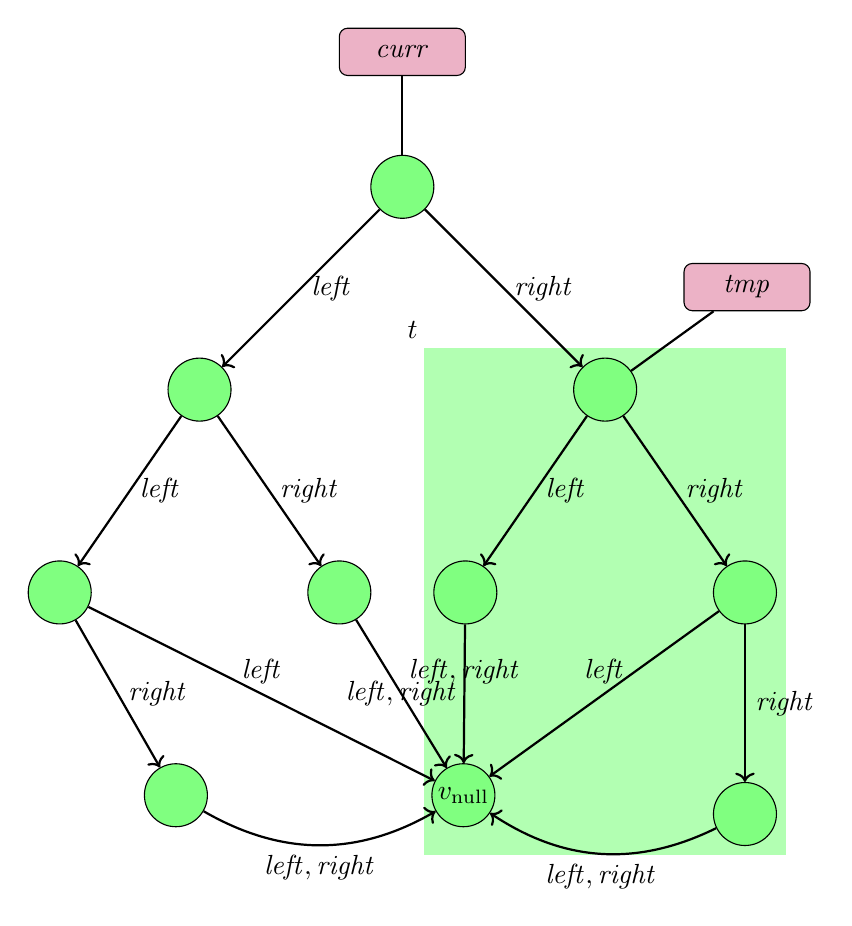
\begin{tikzpicture}[node distance=2 and 2]
		\node[node] (r)  {};
		\node[var] (curr) [above=of r] {$\mathit{curr}$};
		\node[node] (r-l) [below left=of r] {};
		\node[node] (r-r) [below right=of r] {};
		\node[node, node distance=2 and 1.2] (r-l-l) [below left=of r-l] {};
		\node[node, node distance=2 and 1.2] (r-l-r) [below right=of r-l] {};
		\node[node, node distance=2 and 1.2] (r-r-l) [below left=of r-r] {};
		\node[node, node distance=2 and 1.2] (r-r-r) [below right=of r-r] {};
		\node[node]                          (r-r-r-r) [below=of r-r-r] {};
		\node[node, node distance=2 and 0.9] (r-l-l-r) [below right=of r-l-l] {};
		\node[var] (tmp)  [above right=of r-r] {$\mathit{tmp}$};
		\node[node, below right=2 and 1 of r-l-r] (null) {$v_{\text{null}}$};
		\draw [connector] (tmp) to (r-r);
		\draw [connector] (curr) to (r);
		\draw [sel] (r) to node[right]{$\mathit{left}$} (r-l) ;
		\draw [sel] (r) to node[right]{$\mathit{right}$} (r-r);
		\draw [sel] (r-l) to node[right]{$\mathit{left}$} (r-l-l);
		\draw [sel] (r-l) to node[right]{$\mathit{right}$} (r-l-r);
		\draw [sel] (r-r) to node[right]{$\mathit{left}$} (r-r-l);
		\draw [sel] (r-r) to node[right]{$\mathit{right}$} (r-r-r);
		\draw [sel] (r-r-r) to node[right]{$\mathit{right}$} (r-r-r-r);
		\draw [sel] (r-l-l) to node[right]{$\mathit{right}$} (r-l-l-r);
		\draw [sel] (r-l-l) to node[above]{$\mathit{left}$} (null);
		\draw [sel] (r-r-r) to node[above]{$\mathit{left}$} (null);
		\draw [sel] (r-l-r) to node{$\mathit{left},\mathit{right}$} (null);
		\draw [sel] (r-r-l) to node[above]{$\mathit{left},\mathit{right}$} (null);
		\draw [sel, bend left] (r-r-r-r) to node[below]{$\mathit{left},\mathit{right}$} (null);
		\draw [sel, bend right] (r-l-l-r) to node[below]{$\mathit{left},\mathit{right}$} (null);

		\begin{scope}[on background layer]
			\node [fill=green!30,fit=(r-r) (r-r-r) (r-r-l) (r-r-r-r),label=125:$t$] {};
		\end{scope}
	\end{tikzpicture}
	}
\end{minipage}%
\begin{minipage}{0.5\textwidth}
	\scalebox{0.64}{
	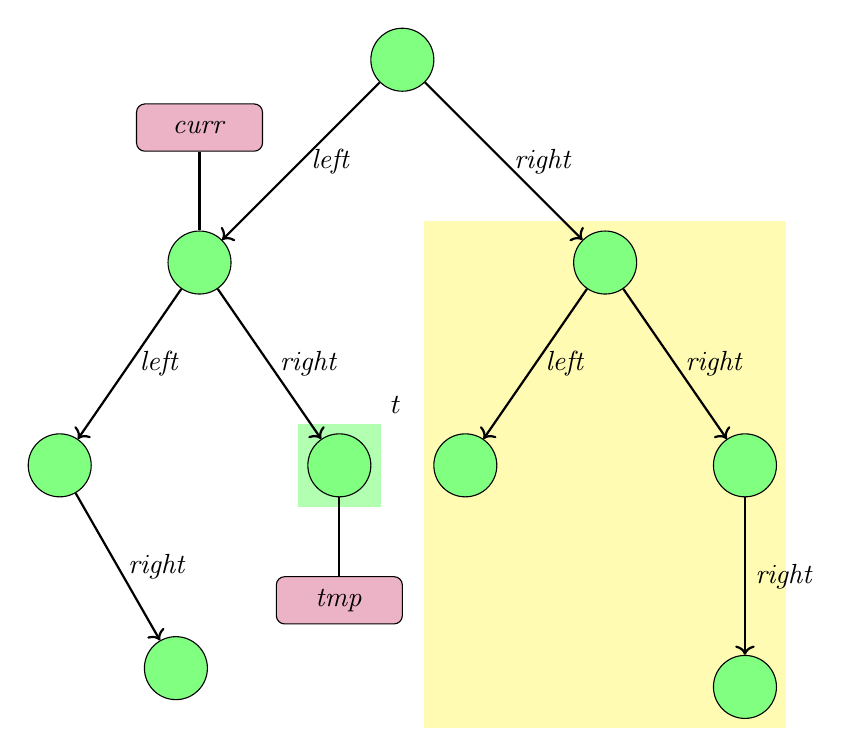
\begin{tikzpicture}[node distance=2 and 2]
		\node[node] (r)  {};
		\node[node] (r-l) [below left=of r] {};
		\node[var] (curr) [above =of r-l] {$\mathit{curr}$};
		\node[node] (r-r) [below right=of r] {};
		\node[node, node distance=2 and 1.2] (r-l-l) [below left=of r-l] {};
		\node[node, node distance=2 and 1.2] (r-l-r) [below right=of r-l] {};
		\node[node, node distance=2 and 1.2] (r-r-l) [below left=of r-r] {};
		\node[node, node distance=2 and 1.2] (r-r-r) [below right=of r-r] {};
		\node[node]                          (r-r-r-r) [below=of r-r-r] {};
		\node[node, node distance=2 and 0.9] (r-l-l-r) [below right=of r-l-l] {};
		\node[var, below=of r-l-r] (tmp) {$\mathit{tmp}$};
		\draw [connector] (tmp) to (r-l-r);
		\draw [connector] (curr) to (r-l);
		\draw [sel] (r) to node[right]{$\mathit{left}$} (r-l);
		\draw [sel] (r) to node[right]{$\mathit{right}$} (r-r);
		\draw [sel] (r-l) to node[right]{$\mathit{left}$} (r-l-l);
		\draw [sel] (r-l) to node[right]{$\mathit{right}$} (r-l-r);
		\draw [sel] (r-r) to node[right]{$\mathit{left}$} (r-r-l);
		\draw [sel] (r-r) to node[right]{$\mathit{right}$} (r-r-r);
		\draw [sel] (r-r-r) to node[right]{$\mathit{right}$} (r-r-r-r);
		\draw [sel] (r-l-l) to node[right]{$\mathit{right}$} (r-l-l-r);

		\begin{scope}[on background layer]
			\node [fill=yellow!30,fit=(r-r) (r-r-r) (r-r-l) (r-r-r-r)] {};
		\end{scope}
		\begin{scope}[on background layer]
			\node [fill=green!30,fit=(r-l-r), label=45:$t$] {};
		\end{scope}
	\end{tikzpicture}
	}
\end{minipage}
\\[1cm]
\begin{minipage}{0.5\textwidth}
	\scalebox{0.6}{
		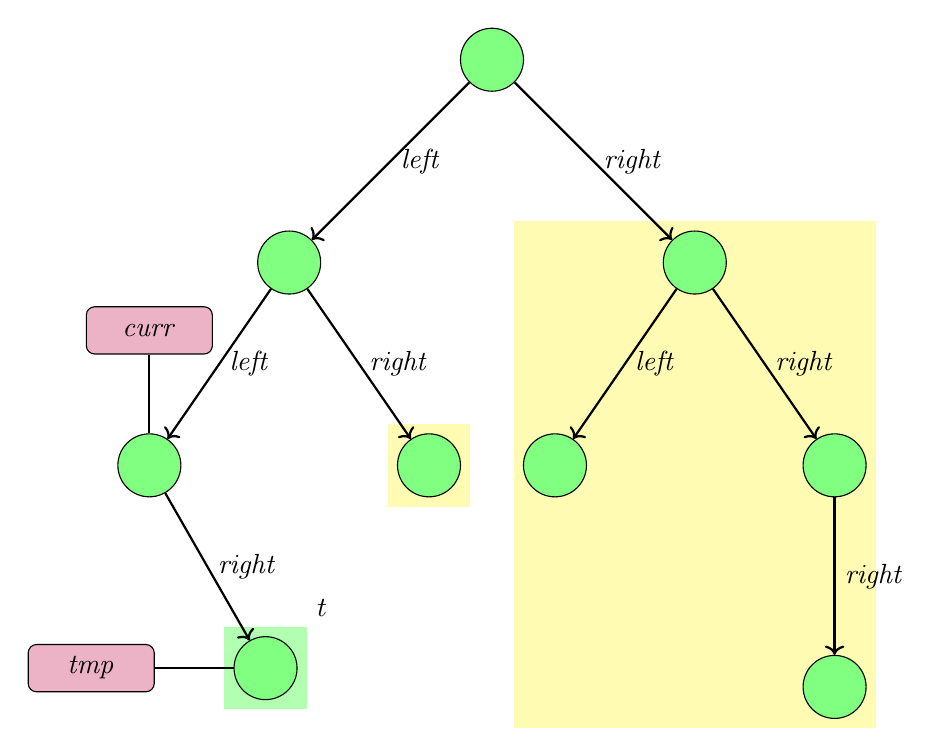
\begin{tikzpicture}[node distance=2 and 2]
			\node[node] (r)  {};
			\node[node] (r-l) [below left=of r] {};
			\node[node] (r-r) [below right=of r] {};
			\node[node, node distance=2 and 1.2] (r-l-l) [below left=of r-l] {};
			\node[var] (curr) [above =of r-l-l] {$\mathit{curr}$};
			\node[node, node distance=2 and 1.2] (r-l-r) [below right=of r-l] {};
			\node[node, node distance=2 and 1.2] (r-r-l) [below left=of r-r] {};
			\node[node, node distance=2 and 1.2] (r-r-r) [below right=of r-r] {};
			\node[node]                          (r-r-r-r) [below=of r-r-r] {};
			\node[node, node distance=2 and 0.9] (r-l-l-r) [below right=of r-l-l] {};
			\node[var, left=of r-l-l-r] (tmp) {$\mathit{tmp}$};
			\draw [connector] (tmp) to (r-l-l-r);
			\draw [connector] (curr) to (r-l-l);
			\draw [sel] (r) to node[right]{$\mathit{left}$} (r-l);
			\draw [sel] (r) to node[right]{$\mathit{right}$} (r-r);
			\draw [sel] (r-l) to node[right]{$\mathit{left}$} (r-l-l);
			\draw [sel] (r-l) to node[right]{$\mathit{right}$} (r-l-r);
			\draw [sel] (r-r) to node[right]{$\mathit{left}$} (r-r-l);
			\draw [sel] (r-r) to node[right]{$\mathit{right}$} (r-r-r);
			\draw [sel] (r-r-r) to node[right]{$\mathit{right}$} (r-r-r-r);
			\draw [sel] (r-l-l) to node[right]{$\mathit{right}$} (r-l-l-r);

			\begin{scope}[on background layer]
				\node [fill=yellow!30,fit=(r-r) (r-r-r) (r-r-l) (r-r-r-r)] {};
			\end{scope}
			\begin{scope}[on background layer]
				\node [fill=yellow!30,fit=(r-l-r)] {};
			\end{scope}
			\begin{scope}[on background layer]
				\node [fill=green!30,fit=(r-l-l-r), label=45:$t$] {};
			\end{scope}
		\end{tikzpicture}
	}
\end{minipage}%
\begin{minipage}{0.5\textwidth}
	\scalebox{0.64}{
		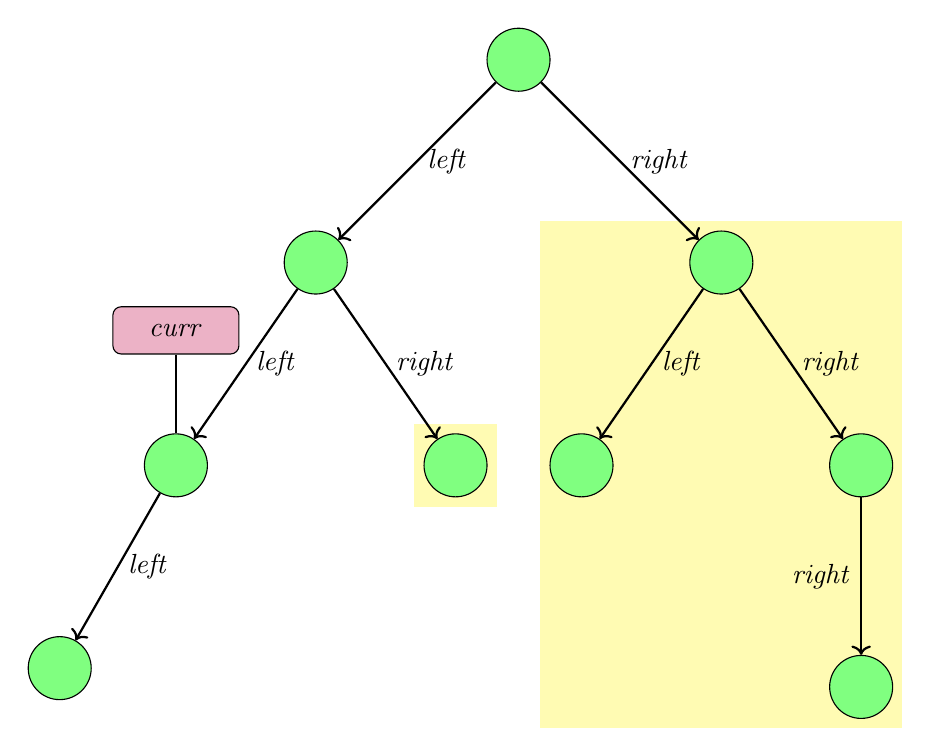
\begin{tikzpicture}[node distance=2 and 2]
			\node[node] (r)  {};
			\node[node] (r-l) [below left=of r] {};
			\node[node] (r-r) [below right=of r] {};
			\node[node, node distance=2 and 1.2] (r-l-l) [below left=of r-l] {};
			\node[var] (curr) [above =of r-l-l] {$\mathit{curr}$};
			\node[node, node distance=2 and 1.2] (r-l-r) [below right=of r-l] {};
			\node[node, node distance=2 and 1.2] (r-r-l) [below left=of r-r] {};
			\node[node, node distance=2 and 1.2] (r-r-r) [below right=of r-r] {};
			\node[node]                          (r-r-r-r) [below=of r-r-r] {};
			\node[node, node distance=2 and 0.9] (r-l-l-r) [below left=of r-l-l] {};
			\draw [connector] (curr) to (r-l-l);
			\draw [sel] (r) to node[right]{$\mathit{left}$} (r-l);
			\draw [sel] (r) to node[right]{$\mathit{right}$} (r-r);
			\draw [sel] (r-l) to node[right]{$\mathit{left}$} (r-l-l);
			\draw [sel] (r-l) to node[right]{$\mathit{right}$} (r-l-r);
			\draw [sel] (r-r) to node[right]{$\mathit{left}$} (r-r-l);
			\draw [sel] (r-r) to node[right]{$\mathit{right}$} (r-r-r);
			\draw [sel] (r-r-r) to node[left]{$\mathit{right}$} (r-r-r-r);
			\draw [sel] (r-l-l) to node[right]{$\mathit{left}$} (r-l-l-r);

			\begin{scope}[on background layer]
				\node [fill=yellow!30,fit=(r-r) (r-r-r) (r-r-l) (r-r-r-r)] {};
			\end{scope}
			\begin{scope}[on background layer]
				\node [fill=yellow!30,fit=(r-l-r)] {};
			\end{scope}
		\end{tikzpicture}
	}
\end{minipage}


		\caption{A graphical representation of the execution of the example
		program for one possible heap state, note that aside from the first step
		selectors which refer to the \textbf{null} value are omitted.}
		\label{fig:BinTreeProgLang}
	\end{figure}
	Some interesting observations can be made:
	\begin{enumerate}
		\item Because of the structure of the binary tree the newly forked
			process can only access the subtrees starting from the parameter
			object (marked in green).
		\item After starting a new process the previously started process cannot
			be referred to anymore since the process identifier is assigned to
			another process. Thus there is no information about any process
			operating on the yellow marked areas of the binary tree.
		\item The last process is joined again, thus it can be assured that it
			has terminated after the join statement. This means especially that
			no process operates on the subtree which is moved from the right hand
			side to the left hand side (as indicated by the absence of a yellow
			mark).
	\end{enumerate}
	The in the following presented analysis of programs relies heavily on
	representing the current state as graph. But in order to approach parallel
	execution of multiple processes which share heap objects and their selectors
	this representation is furtherly enriched. In order to account which parts
	of the heap are accessible by multiple processes it is locally logged for
	the selectors to which processes these are visible.

\newpage
\section{Permission Model}
	\label{sec:pm}
	As stated above it is locally accounted for which process a selector is
	accessible. The main goal of the analysis is to state that the execution
	of a program is \emph{data race free}. Where data race refers to the
	situation that two processes access a shared value at the same time and at
	least one of the processes alters the value. This implies a dependency of
	both actions with each other. For a proper analysis all interleaving have
	to be examined (see \cite[pp. 77-80]{PrinciplesOfModelChecking} for
	details). \emph{Data race freedom} describes the absence of data races which
	can be guaranteed as long the following two conditions are
	met\footnote{this can be easily derived from the explanation of safe
		concurrency in \cite{SeparationLogic}}:
	\begin{itemize}
		\label{itemize:invariants}
		\item If two or more parallel processes access a value it must not be
			altered.
		\item If one process alters a value it must have at this time exclusive
			access to it.
	\end{itemize}
	The accounting is realised in form of \emph{permissions}. Permissions are
	used to model access restrictions in order to ensure
	\begin{enumerate*}[label=(\arabic*)]
		\item that write access is exclusive and
		\item that if other processes might access the same value at the same
			time both are restricted to read access.
	\end{enumerate*}
	Permissions were already introduced for other modelling techniques for heaps
	like \emph{separation logic} \cite{SeparationLogic}. There different models
	for permissions are examined like \emph{fractional permissions} or
	\emph{counting permissions}. All these models share the property that there
	is one distinguishable permission representing exclusive access on a value.
	From this access ticket for one value multiple other access tickets on this
	value can be derived which then causes all these accesses to become read
	only. Furthermore derived access tickets can be returned until there exists
	only one access tickets which then again grants permission to alter the
	given value.
	For fractional permission it is possible that once derived
	tickets can be split indefinitly on demand to generate as many access
	tickets as needed. On the other hand for counting permissions there is one
	distinguishable permission per value from which further access tickets are
	derived. Every derived access ticket is accounted for and can be returned to
	this distinguishable permission.
	In the following course an approach is chosen which is closer
	connected with \cite{FractionalPermissions} and combines both presented
	concepts of \emph{fractional permissions} and \emph{counting permissions}
	and formalises ideas from \cite{NollJansenDraft}.

	Fundamentally two different \emph{permissions} are distinguished:
	\begin{itemize}
		\item $\mathit{WR}$ - denotes that this value can be altered.
		\item $\mathit{RD}$ - denotes a shared access, which restricts to
			reading only.
	\end{itemize}
	These permissions represent access rights where $\mathit{WR}$ is the
	distinguishable value representing exclusive access. From both permissions
	it is possible to derive further access tickets which are locally
	accounted and deleted if these tickets are returnded. Therefore
	the different forked processes are uniquely identified and this
	identification is used to account derived access tickets. Additionally it is
	possible to transfer $\mathit{WR}$ tickets completely. For the
	identification of forked processes the programming language relies on values
	from $\PI$. As it can be seen from the grammar of the programming language
	it is possible that
	multiple process identifiers from $\PI$ can refer to the same actual process
	as it can be easily seen by the following example:
	\begin{lstlisting}
$t_{1}$ = fork(traverse($\mathit{tmp}$));
$t_{2} = t_{1}$;
join($t_{2}$)
	\end{lstlisting}
	Here $t_{1}$ and $t_{2}$ refer to the same forked process. The join
	statement takes any of these possible process identifier to synchronise with
	the corresponding process. In order to account permissions
	given to processes \emph{tokens} are introduced. Tokens are sets of $\PI$
	which refer to the same process. Thus, for every token $T$ always holds that
	$T\subseteq \PI$ and the set of all possible tokens is simply the powerset
	of the process identifiers ($\mathbb{P}(\PI)$). For every shared value
	the permission that it held initially is kept as well as a set of tokens
	that represent all derived tickets to the process that can access this
	value. Recall that variables and process identifiers are considered process
	exclusive and only heap objects and selectors can be shared. Furthermore the
	presented analysis focuses on structural analysis of the heap and therefore
	only consideres selectors as data of heap objects.
	
	In order to formalises these ideas \emph{\acp{PE}} are introduced in
	the following. These consist of a so called $\mathit{BasePerm}$ which
	represents the \emph{permission} that was originally granted and a set of
	tokens for derived permissions.

	For an example consider Figure \ref{fig:BinTreeProgLangPerm}, which mirrors
	the previous example from Figure \ref{fig:BinTreeProgLang} but added
	permissions to the selectors. Imagine all selectors are initially equipped
	with a $\mathit{WR}$ permission. For the part of the heap that the newly
	forked process may access the token $\{t\}$ is added to the permissions.
	\begin{figure}
	\begin{center}\input{tikz/BinTreeProgLangPerm}\end{center}
		\caption{State of the first iteration of the heap shown in Figure
			\ref{fig:BinTreeProgLang} with additional permissions on every
		selector, empty $\mathit{PermSets}$ are omitted, $\mathit{left}$ and
		$\mathit{right}$ are shortened to $l$ and $r$ respectively. For two
		selectors that are represented by one edge the permission for those is
		written only once.}
		\label{fig:BinTreeProgLangPerm}
	\end{figure}
	As already observed in the second iteration of the example from Figure
	\ref{fig:BinTreeProgLang} the information if a process still operates on a
	certain part of the heap is lost. Especially it is impossible to retrieve
	any information of the status of the once forked process because the
	synchronisation mechanism (join statement) demands an identifier referring
	to the process which no longer exists. In this case the derived access
	tickets are considered permanently lost. In order to model this for
	permissions two additional $\mathit{BasePerm}$ besides
	$\mathit{WR},\mathit{RD}$ are introduced: $\mathit{WR^{\ast}}$ and
	$\mathit{RD^{\ast}}$ which indicate that the initially granted permission
	can never be fully returned since the information about any parallel
	executing processes is lost. The following definition formalises these
	observations:
	\begin{definition}[Permission Expression]
		A \emph{\acl{PE}} is a term of the form
		$$\mathit{BasePerm} - \mathit{PermSet}$$
		where $\mathit{BasePerm}\in
		\{\mathit{WR},\mathit{WR^\ast},\mathit{RD},\mathit{RD^\ast}\}$.
		And $\mathit{PermSet}\subseteq\mathbb{P}(\PI)$.
	\end{definition}
	For convenience an empty $\mathit{PermSet}$ and a $\mathit{PermSet}$
	after $\mathit{RD^\ast}$ or $\mathit{WR^\ast}$ as $\mathit{BasePerm}$ might
	be omitted if it is clear from the context that this information is not
	needed.  Sometimes for a $\mathit{BasePerm}$ $\rho$ and a $\mathit{PermSet}$
	$\Phi$ and $T\in\mathbb{P}(\PI)$
	$\rho - \Phi - T$ is written for $\rho - \Phi\cup\{T\}$.
	In addition a \emph{\ac{PE}} with an empty $\mathit{PermSet}$ is called
	\emph{simple}. The set of all \emph{\acp{PE}} over $\PI$ is denoted by
	$\mathit{PES}_{\PI}$. Note that for a finite set $\PI$ $\mathit{PES}_{\PI}$
	is finite as well.

	For now it was always considered that the process only reads the part of the
	heap it has access to. But as it is introduced later on there also will be a
	way to specify for a process that it might alter certain selectors. In order
	to model that this part of the heap must not be accessed anymore because the
	access ticket is completely submitted to the forked process. This is
	achieved by substituting this part of the heap that might be altered by a
	placeholder.
	This placeholder ``hides'' parts of the heap so it can not be accessed.
	Upon joining this process again the placeholder is additionally used to
	identifiy where the part of the heap to which the access ticket is
	transferred to is returned.
	For the program from Listing \ref{lst:ExampleProgram} consider that the
	forked process might demand write access on the right subtree of its
	parameter. Then the substitution of this subtree by a placeholder can be
	seen in Figure \ref{fig:BinTreeProgLangPermReplacement}. Note that the
	placeholder is connected to the node which can still be accessed from the
	original heap but is also the node that the parameter of $\mathit{traverse}$
	pointed to and to the \textbf{null} node.
	\begin{figure}
	\begin{center}\begin{tikzpicture}[node distance=2 and 2]
	\node[node] (r)  {};
	\node[var] (curr) [above=of r] {$\mathit{curr}$};
	\node[node] (r-l) [below left=of r] {};
	\node[node] (r-r) [below right=of r] {};
	\node[node, node distance=2 and 1.2] (r-l-l) [below left=of r-l] {};
	\node[node, node distance=2 and 1.2] (r-l-r) [below right=of r-l] {};
	\node[node, node distance=2 and 1.2] (r-r-l) [below left=of r-r] {};
	\node[node, node distance=2 and 0.9] (r-l-l-r) [below right=of r-l-l] {};
	\node[he, node distance=2 and 0.9] (Nt) [below right=of r-r] {$N_{\{t\}}$};
	\node[node, below right=2 and 1 of r-l-r] (null) {$v_{\text{null}}$};
	\draw [connector] (curr) to (r);
	\draw [connector] (r-r) to (Nt);
	\draw [connector, bend left=50] (Nt) to (null);
	\draw [sel] (r) to node[left]{$l_{\mathit{WR}}$} (r-l) ;
	\draw [sel] (r) to node[right]{$r_{\mathit{WR}}$} (r-r);
	\draw [sel] (r-l) to node[left]{$l_{\mathit{WR}}$} (r-l-l);
	\draw [sel] (r-l) to node[right]{$r_{\mathit{WR}}$} (r-l-r);
	\draw [sel] (r-r) to node[right] {$l_{\mathit{WR} - \{\{t\}\}}$} (r-r-l);
	\draw [sel] (r-l-l) to node[right]{$r_{\mathit{WR}}$} (r-l-l-r);
	\draw [sel] (r-l-l) to node[above]{$l_{\mathit{WR}}$} (null);
	\draw [sel] (r-l-r) to node{$(l,r)_{\mathit{WR}}$} (null);
	\draw [sel] (r-r-l) to node[above right]{$(l,r)_{\mathit{WR} - \{\{t\}\}}$}
		(null);
	\draw [sel, bend right] (r-l-l-r) to node[below]{$(l,r)_{\mathit{WR}}$}
		(null);

	\begin{scope}[on background layer]
		\node[fill=green!30,fit=(r-r) (r-r-r) (r-r-l) (r-r-r-r),label=125:$t$]{};
	\end{scope}
\end{tikzpicture}

\end{center}
		\caption{State of the first iteration of the heap shown in figure
			\ref{fig:BinTreeProgLang} with permissions as well as partially
		substitution with a placeholder.}
		\label{fig:BinTreeProgLangPermReplacement}
	\end{figure}

\newpage
\section{Hypergraphs as Heap Representation}
	In order to formalise the intuitive graph representation from the examples
	above \emph{\acp{HG}} are introduced in the following. This follows the
	general approach presented in \cites{LocalGreibachNormalForm}
	{InductivePredicates}{InformalGraphGrammars}{fmsd}. Intuitively, an
	\emph{\ac{HG}} is the same as a normal graph, it consists of a set of nodes
	and edges, but an edge in an \emph{\ac{HG}} is called hyperedge and can
	connect arbitrarily many nodes instead of only two. Furthermore the used
	\emph{\acp{HG}} will be labeled, thus there is a function $\lab$ which
	assigns a label to every hyperedge. The possible labels come from a set
	$\Sigma$.  Then an \emph{\ac{HG}} can be formally defined as follows:
	\begin{definition}[Hypergraph]
		Let $\Sigma$ be a set of labels and let $V$ be a finite
		set of nodes, $E$ a finite set of edges.
		$\con: E\rightarrow V^{*}$ maps every edge to the sequence of
		connected nodes, $\lab: E\rightarrow\Sigma$ labels every edge.
		Further let $ext\in V^{*}$ denote a possibly empty
		sequence ($\varepsilon$) of nodes and $\perm: E\rightarrow \PES$. An
		\emph{\ac{HG}} $H$ is a tupel
		\begin{equation*}
			H=(V, E, \con, \lab, \ext, \perm)
		\end{equation*}
	\end{definition}
	The set of all hyperedges with the labels $\Sigma$ and process identifier 
	$\PI$ is denoted by $\HG$. Two \emph{\acp{HG}} are called \emph{isomorphic}
	if they are equivalent modulo renaming of edges and nodes. Isomorphic
	\emph{\acp{HG}} are not distinguished in the following.

	In order to represent states of the heap the objects in the heap will be
	represented as nodes. Variables are represented by hyperedges that are
	only connected to the node that represents the value of the variable. Such
	a hyperedge that is connected to only one node is called \emph{unary}.
	Selectors are modelled as binary hyperedges between nodes, which are
	interpreted as directed from the first node of the connection sequence to
	the second one. Furthermore parts that are given away to other processes
	are substituted by hyperedges. For the hyperedges that represent parts of
	the heap for which access tickets are transferred a set of labels is
	introduced as
	\begin{equation*}
		\mathbb{T} = \{N_{T} \mid T\in\mathbb{P}(\PI)\}
	\end{equation*}
	States of the heap can now be represented as $H\in\HG$ where
	$\Sigma = \Var\uplus\Sel\uplus\mathbb{T}$, but of course not all those
	\emph{\ac{HG}} $H$ represent valid heaps because it is e.g. possible that
	every object might have multiple outgoing edges labeled with the same
	selector. Thus some restrictions are enforced in order to represent valid
	states of a heap which are called \emph{\acp{HC}}, namely:
	\begin{itemize}
		\item There is exactly one distinguishable node $v_{\text{null}}$
			representing the \textbf{null} value. $v_{\text{null}}$ has no
			outgoing selectors.
		\item There is exactly one unary hyperedge for every variable.
		\item Edges labeled by a selector are binary hyperedges.
		\item For every node there is at most one outgoing edge per
			selector.
	\end{itemize}
	Note that every object is universally typed. Thus, all objects have
	initially an outgoing edge for every selector. But of course some of these
	edges
	can be \enquote{hidden} within a hyperedge representing parts of the heap
	for which $\mathit{WR}$ permissions are transferred to another process. As
	it is possible that the reference to the process that operates exclusively
	on the selectors is lost, these selectors can permanently be removed from
	the heap state.
	This leads to the following formal definition for \emph{\acp{HC}}:
	\begin{definition}[Heap Configuration]
		A \emph{\acl{HG}}\\
		$H = (V, E, \mathit{con}, \mathit{lab}, \mathit{ext}, \mathit{perm}) \in
		\HG$ is called a \emph{\acl{HC}} if
		\begin{itemize}
			\item $\Sigma = \mathit{Var}\biguplus\mathit{Sel}\biguplus \mathbb{T}$
			\item $v_{\text{null}}\in V$ and
				$\nexists e\in E.\lab_{H}(e)\in\Sel\land
				\con_{H}(e)(1)=v_{\text{null}}$
			\item $|\con_{H}(e)| = 1$ for all $e\in E$ with $\lab_{H}(e)\in
				\mathit{Var}$
			\item $|\con_{H}(e)| = 2$ for all $e\in E$ with $\lab_{H}(e)\in
				\mathit{Sel}$
			\item $\forall v\in\mathit{Var}.\exists e\in E. \lab_{H}(e) = v$
			\item $\forall v\in\mathit{Var}, e,e'\in E.
				v = \lab_{H}(e) = \lab_{H}(e') \rightarrow e = e'$
			\item $\forall s\in\mathit{Sel}, e,e'\in E.
				\con_{H}(e)(1) = \con_{H}(e')(1) \land
				s = \lab_{H}(e) = \lab_{H}(e') \rightarrow e = e'$
		\end{itemize}
	\end{definition}
	The set of all \emph{\ac{HC}} over $\Sigma$ and
	$\PI$ is denoted by $\HC$.

	Furthermore the following notion is defined for $\rho\in\PES$ which
	collects all edges of the \ac{HG} with permission $\rho$:
	\begin{equation*}
		E^{H}_{\rho} = \{e\in E_{H}\mid\perm_{H}(e) = \rho\}
	\end{equation*}

\newpage
\section{Concrete Semantics}
	Because \emph{\acp{HG}} are used to represent the current state of the heap
	the semantics of the programming language are modelled in
	terms of graph transformations. Therefore the different statements of a
	program are connected with changes of the shape of the hypergraph
	representing the state of the heap. In the following the necessary graph
	transformations which are based on presented transformations of \cite{fmsd}
	for modelling the semantics are presented. This is done in two separate
	parts where firstly structural changes are discussed and secondly
	transformations that regard the \emph{\acp{PE}} of the graph.
\subsection{Graph Transformations}
\label{sec:graphtrans}
	The structural graph transformations are presented in the following:
	\begin{itemize}
		\item $H[+v]$ adds a new fresh node $v$ to $H$, which is of universally
			type, thus there are edges attached to for all \emph{selectors}
		\item $H[\setminus E']$ removes the set of edges $E'$ from $H$
		\item $H[x\hookrightarrow v]$ connects one $x$ labeled edge with $v$,
			where $x\in\Var$
		\item $H[u\xhookrightarrow{s} v]$ connects one $s$ labeled edge
			from the node $u$ to the node $v$
		\item $H[+_{\rho}n\rightrightarrows v_1\cdots v_m]$ adds a fresh $n$
			labeled edge with \emph{permission} $\rho$ connected to
			$v_1\cdots v_m$
	\end{itemize}
	Formally these transformations are defined as follows, where $v$ is a new
	node and $e,e_{1},\dots$ are new edges:
	\begin{center}
		\begin{tabular}{lcl}
			$H[+v]$ & $=$ &
				$\begin{aligned}
					(&V_{H}\uplus\{v\},
					E_{H}\uplus\{e_{1},\dots,e_{|\mathit{Sel}|}\},\\
					&\con_{H}\cup\{e_{1}\mapsto vv_{\text{null}},\dots,
					e_{|\mathit{Sel}|}\mapsto vv_{\text{null}}\},\\
					&\lab_{H}\cup\{e_1\mapsto\mathit{enum}_{\mathit{Sel}}(1),\dots,
					e_{|\mathit{Sel}|}\mapsto\mathit{enum}_{\mathit{Sel}}
					(|\mathit{Sel}|)\},\\
					&\ext_{H},
					\perm_{H}\cup\{e_{1}\mapsto\mathit{WR},\dots,
					e_{|\mathit{Sel}|}\mapsto\mathit{WR}\})\\
				\end{aligned}$\\
			\hline
			$H[\setminus E']$ & $=$ &
				$\begin{aligned}
					(&V_H,E_H\setminus E',
					 \con_H\upharpoonright (E\setminus E'),
					 \lab_H\upharpoonright (E\setminus E'),\\
					 &\ext_H,
					 \perm_H\upharpoonright (E\setminus E'))
				\end{aligned}$\\
			\hline
				$H[x\hookrightarrow u]$ & $=$ &
				\begin{minipage}{4.5cm}
					$\begin{aligned}
						(&V_{H},E_{H},\\
						 &\mathit{con}_{H}[e\mapsto u],\\
						 &\mathit{lab}_{H},\mathit{ext}_{H},\mathit{perm}_{H})
					\end{aligned}$
				\end{minipage}%
				\begin{minipage}{5cm}
					for one $e$ with $\lab_{H}(e) = x$, if such an $e$ exists
				\end{minipage}\\
			\hline
				$H[u\xhookrightarrow{s} u']$ & $=$ &
				\begin{minipage}{4.5cm}
					$\begin{aligned}
						(&V_H,E_H,\\
						 &\mathit{con}_H[e\mapsto uu'],\\
						 &\mathit{lab}_H,\mathit{ext}_H,\mathit{perm}_H)
					\end{aligned}$
				\end{minipage}%
				\begin{minipage}{5cm}
					if there is $e$ with $\lab_{H}(e) = s$ and $\con_{H}(e)(1) = u$
					and $u,u'\in V_{H}$
				\end{minipage}
			\\
			\hline
			$H[+_{\rho}n\rightrightarrows v_1\cdots v_n]$ & $=$ &
			$\begin{aligned}
				(&V_H,E_H\uplus\{e\},
				 \con_H\cup\{e\mapsto v_1\cdots v_n\},\\
				 &\lab_H\cup\{e\mapsto n\},
				 \ext_H,
				 \perm_H\cup\{e\mapsto\rho\})
			\end{aligned}$\\
		\end{tabular}
	\end{center}
	The few more transformation which focus on various aspects of the
	\emph{permissions} are also introduced below:
	\begin{itemize}
		\item $H[\downarrow t]$ denotes that $t\in\PI$
			does not longer identify a certain process (for example by reassigning
			$t$)
		\item $H[\leftarrow T]$ denotes that the \emph{permissions} for
			$T\in\mathbb{P}(\PI)$ are returned
		\item $H[t = t']$ is used to describe that for
			$t,t'\in\PI$ $t$ now identifies the same
			process as $t'$
		\item $H[E - T]$ denotes that for the edges in $E$ the token $T$ is added
			to the $\mathit{PermSet}$ of the \emph{permissions}
	\end{itemize}
	The following definitions formalise these intuitions:
	\begin{definition}[Dropped Thread Variable]
		For an \emph{\ac{HC}} $H$, $t\in\PI$ let
		$E_{\text{remove}}\subseteq E_{H}$ be all edges $e$ such that
		$\lab_{H}(e) = N_{\{t\}}$. Then $H[{\downarrow{t}}]$ denotes the \ac{HC}
		with:
		\begin{equation*}
			H[{\downarrow{t}}]= (V_{H},
			\underbrace{E_{H}\setminus E_{\text{remove}}}_{=: E'},
			\con_{H} \upharpoonright E',
			\lab' \upharpoonright E', \perm'
			\upharpoonright E')
		\end{equation*}
		where $\lab'$ mirrors $\lab_{H}$ except of all edges $e$ such that
		$\lab_{H} = N_{T}\in\mathbb{T}$ where holds
		$\lab'(e) = N_{(T\setminus \{t\})}$. And for all edges $e$ with
		$\perm_{H}(e) = \rho_{e} - \Phi_{e}$ $\perm'(e)$ is defined as follows:
		\begin{equation*}
			\perm'(e) =
			\begin{cases}
				\mathit{WR^\ast} - \Phi_{e}\setminus\{\{t\}\}&\text{if }
				\rho_{e}\in\{\mathit{WR},\mathit{WR^\ast}\} \text{ and }
				\{t\}\in\Phi_{e}\\
				\mathit{RD^\ast} - \Phi_{e}\setminus\{\{t\}\}&\text{if }
				\rho_{e}\in\{\mathit{RD},\mathit{RD^\ast}\} \text{ and }
				\{t\}\in\Phi_{e}\\
				\rho_{e} - \{T\setminus\{t\}\mid T\in\Phi_{e}\} &\text{otherwise}
			\end{cases}
		\end{equation*}
	\end{definition}
	Note that all edges labeled with $N_{\{t\}}$ are removed. This is because
	these edges are the placeholder for the part of the heap that the process
	$t$ referred to might alter. Thus, in order to ensure data race freedom this
	part of the heap has to be exclusively accessible by this process. Because
	the process which operates on this part of the heap can never be rejoined
	(the token is a singleton set only containing $t$, thus only $t$ refers to
	this process and is reassigned) all these nodes and edges
	must never be accessed. To achieve this the placeholder is removed which
	removes this part of the heap permanently. Furthermore all tokens containing
	$t$ are updated in order to indicate that $t$ no longer identifies the same
	process as the other process identifier of this token. For those
	$\mathit{PermSets}$ that contain the token $\{t\}$ the $\mathit{BasePerm}$
	is \enquote{starred} in order to indicate that, since there is no further
	reference to the process the corresponding access token can never be
	returned. And this implies that the $\mathit{BasePerm}$ can never be fully
	recovered.
	\begin{definition}[Returned Token]
		For $H\in\HC$, $T\in\mathbb{P}(\PI)$
		\begin{equation*}
			H[\leftarrow T] = (V_{H}, E_{H}, \con_{H}, \lab_{H}, \ext_{H}, \perm')
		\end{equation*}
		with $\perm'(e) = \rho - \Phi\setminus\{T\}$ where
		$\perm_{H}(e) = \rho -\Phi$.
	\end{definition}
	Note that simply the token $T$ is removed from all the $\mathit{PermSets}$.
	The return of parts of the heap that the process identified by $T$ (or
	rather all $t\in T$) had exclusive access on is dealt with separately.
	\begin{definition}[Thread Variable Assignment]
		For $H\in\HC$ and $t,t'\in\PI$ let
		$\Phi_{t'} = \{ T\in\Phi \mid t'\in T\}$ denote the set of all
		tokens in a $\mathit{PermSet}$ $\Phi$ which contain the process
		identifier $t'$. Then
		\begin{equation*}
			H[t = t'] = (V_{H[\downarrow t]}, E_{H[\downarrow t]},
				\con_{H[\downarrow t]}, \lab',
				\ext_{H[\downarrow t]}, \perm')
		\end{equation*}
		where $\lab'$ mirrors $\lab_{H[\downarrow t]}$ except for all
		$e\in E_{H[\downarrow t]}$ with $\lab_{H[\downarrow t]}(e) = N_{T}$ and
		$t'\in T$ where $\lab'(e) = N_{T\cup\{t\}}$. And
		$\perm'(e)=\rho-(\Phi\setminus\Phi_{t'}\cup
		\{T\cup\{t\}\mid T\in\Phi_{ t'}\})$ if
		$\perm_{H[\downarrow t]}(e) = \rho-\Phi$.
	\end{definition}
	Note that for the assignment the reassigned identifier is previously
	dropped since its original value will be lost after the assignment. And
	the set of tokens for all $\mathit{PermSets}$ that do not contain the
	process identifier $t'$ are simply preserved. To thoses tokens that contain
	$t'$ as process identifier $t$ is added since $t$ identifies from now on the
	same process as $t'$.
	\begin{definition}[Add Token to Edge]
		For $H\in\HC$, $T\in\mathbb{P}(\PI)$ and $E\subseteq E_{H}$
		\begin{equation*}
			H[E-T] = (V_{H}, E_{H}, \con_{H}, \lab_{H}, \ext_{H}, \perm')
		\end{equation*}
		where
		\begin{equation*}
			\perm'(e) =
			\begin{cases}
				\perm_{H}(e) - T &\text{if }e\in E\\
				\perm_{H}(e)     &\text{otherwise}\\
			\end{cases}
		\end{equation*}
	\end{definition}
	The token $T$ is simply added to all $\mathit{PermSets}$ of edges in $E$.
	\subsection{Semantics}
	In the following the semantics of programs are defined
	by graph transformations. Therefore some relations over nodes in
	\emph{\acp{HG}} are defined as follows:
	\begin{itemize}
		\item $v\xhookrightarrow{s}_{\rho}v'$ states that the node $v$ is
			connected to the node $v'$ by an edge labeled with $s\in\mathit{Sel}$
			and the permission $\rho$
		\item $x\hookrightarrow_{\rho}v$ denotes that there is an edge labeled
			with $x\in\mathit{Var}$ and the permission $\rho$ which is connected
			to the node $v$
	\end{itemize}
	For both relations the permission might be omitted to indicate that one
	permission $\rho$ exists such that the relation holds.

	At first the semantics of pointer expressions are examined.
	This is, evaluating a pointer expression under an \emph{\ac{HC}}
	$H\in\mathit{HC}_\Sigma$ ($\llbracket\cdot\rrbracket_H$). Intuitively, this
	means that variables are identified with the node the edge labeled with the
	variable is attached to, the \textbf{null} value is identified with
	$v_{\text{null}}$ and dereferencing a selector of the object corresponds to
	following the outgoing edge from a node labeled by this selector. There are
	two possible errors: firstly, dereferencing anything from the \textbf{null}
	value and secondly, accessing a selector which is not there. The second case
	indicates that a selector is accessed although another process demands
	exclusive access. Because of the universal type of every node the only
	possible way a selector is absent is because it is hidden behind a
	placeholder for another process or removed because the reference to the
	corresponding process is lost. Such an error is indicated by returning an
	error symbol $\bot$. Formally this leads to the following:
	\begin{center}
		\begin{tabular}{lcl}
			$\llbracket \textbf{null}\rrbracket_H$ & $=$ & $v_{\text{null}}$\\
			&&\\
				$\llbracket x\rrbracket_{H}$ & $=$ & $v$\hspace{0.65cm} with
				$x\hookrightarrow v$\\
			&&\\
			$\llbracket x.s\rrbracket$ & $=$ & $
			\begin{cases}
				v    &\text{if } \llbracket x\rrbracket_{H}\xhookrightarrow{s} v\\
				\bot &\text{otherwise}\\
			\end{cases}
			$\\
		\end{tabular}
	\end{center}
	Note that for an \emph{\ac{HC}} these semantics are well defined since
	every node has maximal one outgoing edge for every selector and for every
	variable exists exactly one edge labeled with it.

	The semantics of conditions are evaluated very intuitively, but where $\bot$
	propagates strictly, i.e. if there is one expression yielding $\bot$ the
	whole evaluation becomes $\bot$. Therefore for pointer expressions
	$p_1,p_2$, and conditions $c_1, c_2$:
	\begin{center}
		\begin{tabular}{lcl}
			$\llbracket p_1 == p_2\rrbracket_H$ & $=$ & $
			\begin{cases}
				\bot &\text{if } \llbracket p_1\rrbracket_H = \bot \text{ or }
					\llbracket p_2\rrbracket_H = \bot \\
				\mathit{true} &\text{if } \llbracket p_1\rrbracket_H =\llbracket
					p_2\rrbracket_H\\
				\mathit{false} &\text{if } \llbracket p_1\rrbracket_H
					\neq\llbracket p_2\rrbracket_H \\
			\end{cases}$\\
			\\
			$\llbracket p_1\;\text{!=}\; p_2\rrbracket_H$ & $=$ & $
			\begin{cases}
				\bot &\text{if } \llbracket p_1\rrbracket_H = \bot \text{ or }
					\llbracket p_2\rrbracket_H = \bot \\
				\mathit{false} &\text{if } \llbracket p_1\rrbracket_H=\llbracket
					p_2\rrbracket_H\\
				\mathit{true} &\text{if } \llbracket p_1\rrbracket_H
					\neq\llbracket p_2\rrbracket_H \\
			\end{cases}$\\
			\\
			$\llbracket c_1\;\&\&\; c_2\rrbracket_H$ & $=$ &
				$\begin{cases}
					\bot &\text{if } \llbracket c_1\rrbracket_H = \bot \text{ or }
					\llbracket c_2\rrbracket_H = \bot\\
					\llbracket c_1\rrbracket_H\land\llbracket c_2\rrbracket_H &
					\text{otherwise}\\
				\end{cases}
					$\\
			\\
			$\llbracket c_1 \;\|\; c_2\rrbracket_H$ & $=$ &
				$\begin{cases}
					\bot&\text{if }\llbracket c_1\rrbracket_H =\bot\text{ or }
				\llbracket c_2\rrbracket_H=\bot\\
					\llbracket c_1\rrbracket_H\lor \llbracket c_2\rrbracket_H
					&\text{otherwise}\\
				\end{cases}$\\
		\end{tabular}
	\end{center}
	This gives the basis to define the semantics for the given programming
	language using a \emph{transition system}:
	\begin{definition}[Semantics of the Programming Language]
		The \emph{semantics} of the individual statements are modelled by a
		\emph{transition relation} of the form
		$\rhd \subseteq
		(\mathbb{S}\cup\{\varepsilon\} \times \mathit{HC}_{\Sigma})^{2}$ where
		$\mathbb{S}$ denotes the language derived by the grammar in
		section \ref{sec:syntax}.
	\end{definition}
	The semantics for the \emph{assignment, allocation, loop, conditional
	and skip statement} can be given by the following rules, where
	$v\hookrightarrow_{\rho} -$ abbreviates
	$\exists v'.v\hookrightarrow_{\rho} v'$ and $v\xhookrightarrow{s}_{\rho} -$
	is expanded to $\exists v'.v\xhookrightarrow{s}_{\rho} v'$:
	\begin{center}
		\label{transitionrules}
		\begin{prooftree}
			\AxiomC{$\llbracket P\rrbracket_H\neq\bot$}
			\AxiomC{$\llbracket x\rrbracket_H\hookrightarrow_{\mathit{WR}} -$}
			\BinaryInfC{$(x = P, H)\rhd (\varepsilon, H[
				\llbracket x\rrbracket_H\hookrightarrow
				\llbracket P\rrbracket_H])$}
		\end{prooftree}
		\begin{prooftree}
			\AxiomC{$\llbracket P\rrbracket_H\neq\bot$}
			\AxiomC{$\llbracket x\rrbracket_H\xhookrightarrow{s}_{\mathit{WR}} -$}
			\BinaryInfC{$(x.s = P, H)\rhd (\varepsilon, H[
			\llbracket x\rrbracket_H\xhookrightarrow{s}
		\llbracket P\rrbracket_H])$}
		\end{prooftree}
		\begin{prooftree}
			\AxiomC{$\llbracket C\rrbracket_H = \text{true}$}
			\UnaryInfC{$(\text{while}(C) \text{ do } S \text{ done}, H)
			\rhd (S;\text{while}(C) \text{ do } S \text{ done}, H)$}
		\end{prooftree}
		\begin{prooftree}
			\AxiomC{$\llbracket C\rrbracket_H = \text{false}$}
			\UnaryInfC{$(\text{while}(C) \text{ do } S \text{ done}, H)
			\rhd (\varepsilon, H)$}
		\end{prooftree}
		\begin{prooftree}
			\AxiomC{$\llbracket C\rrbracket_H = \text{true}$}
			\UnaryInfC{$(\text{if}(C) \text{ then } S_1
			\text{ else } S_2 \text{ fi}, H)\rhd(S_1,H)$}
		\end{prooftree}
		\begin{prooftree}
			\AxiomC{$\llbracket C\rrbracket_H = \text{false}$}
			\UnaryInfC{$(\text{if}(C) \text{ then } S_1
			\text{ else } S_2 \text{ fi}, H)\rhd(S_2,H)$}
		\end{prooftree}
		\begin{prooftree}
			\AxiomC{$\llbracket x\rrbracket_H \hookrightarrow_{\mathit{WR}} -$}
			\UnaryInfC{$(\text{new}(x), H)\rhd(\varepsilon,H[+v]
			[x\hookrightarrow v])$}
		\end{prooftree}
		\begin{prooftree}
			\AxiomC{}
			\UnaryInfC{$(\text{skip}, H)\rhd(\varepsilon,H)$}
		\end{prooftree}
		\begin{prooftree}
			\AxiomC{$(S_1,H)\rhd(S_{1}', H')$}
			\UnaryInfC{$(S_1;S_2, H)\rhd(S_{1}';S_2,H')$}
		\end{prooftree}
		\begin{prooftree}
			\AxiomC{$t,t'\in\PI$}
			\UnaryInfC{$(t = t', H)\rhd(\varepsilon, H[t = t'])$}
		\end{prooftree}
		\begin{prooftree}
			\AxiomC{}
			\UnaryInfC{$(\varepsilon;S, H)\rhd(S,H)$}
		\end{prooftree}
	\end{center}
	Note that for operations that change an edge a $\mathit{WR}$ permission on
	that edge is expected. Furthermore every statement that does not have a
	fitting transition rule yields explicitly $\bot$.
	Since fork and join are more complex they are examined in more detail below.

	\subsection{Fork}
	\label{sec:fork}
	As described previously fork creates a process and provides it with
	parameters.This is similar to procedure calls modelled in
	\cite{ProcedureSummaries}.
	In the following two types of parameters are distinguished:
	\begin{itemize}
		\item \emph{Formal parameters}, which belong to the newly created process
		\item \emph{Actual parameters}, which belong to the process executing the
			fork statement
	\end{itemize}
	In the call of a fork statement the actual parameters are provided to
	the newly created process and are identified with formal parameters.
	Thus the new process initially only knows the nodes identified by the actual
	parameters and can now access other nodes via the different selectors.
	The subgraph that can be accessed in this way is called
	\emph{reachable}. The concept of \emph{reachability} will be later on
	introduced formally but partially relies on the abstraction that is
	introduced in Section \ref{sec:abstraction} and is therefore here only given
	as the set $\reach(v_1,\dots,v_n)$ which denotes all edges that are
	considered to be reachable from the nodes $v_1,\dots,v_n$.\footnote{actually
		the set $\reach(v_1,\dots,v_n)$ is a superset of the actual reachable
		edges, but because it covers at least all actual reachable edges the
	soundness of the model for the semantics is ensured}

	Reconsider the example from Listing \ref{lst:ExampleProgram} and Figure
	\ref{fig:BinTreeProgLang} on page \pageref{fig:BinTreeProgLang} where it was
	observed that \emph{forking} a new process and assigning it to a process
	identifier potentially causes to lose the possibility to refer to the
	process the process identifier identified before. In order to model this
	loss of information the semantics rely on a corresponding graph
	transformation ($H[\downarrow t]$). Another aspect of the fork
	statement is that as demonstrated in Figure
	\ref{fig:BinTreeProgLangPermReplacement} it is possible that a write access
	ticket is completely transferred to the \emph{forked} process. As mentioned
	in Section \ref{sec:introduction} the behaviour of processes and especially
	which parts of the heap the process might alter is defined in a
	\emph{contract}.
	These contracts consist of a \emph{precondition}, the set of edges which the
	process might alter and a \emph{postcondition}.
	The precondition is the representation of the context from which the process
	is forked from. The postcondition is the representation of the
	\emph{heap} that resulted from the execution of the process started from an
	initial heap state.
	This initial heap state is obtained by a \emph{transformation} of the
	precondition which is examined later on.
	Firstly, as mentioned in Section \ref{sec:ProgLang} it is expected
	that every process has its own variables as well as process identifier.
	W. l. o. g. the heap state for every forked process can be described as an
	\emph{\ac{HC}} over the set $\PI'$ and
	$\Sigma' = \Sel\uplus\mathbb{T}'\uplus\Var'$ with renaming of variables and
	process identifier as well as limiting the used variables and process
	identifier to subsets of $\Var'$ and $\PI'$. Especially it holds that
	$\Var\cap\Var'=\emptyset$ and $\PI\cap\PI'=\emptyset$.
	Secondly, the precondition is examined as a representation which is isomorph
	to the reachable subgraph. Therefore it is assumed that the precondition is
	a \emph{\ac{HG}} from $\HG$. On the other hand the postcondition is the
	result of the computation of the forked process and therefore represented as
	\emph{\ac{HG}} from $\mathit{HG}_{\Sigma'}^{\PI'}$. And this computation of
	the forked process ensures that only edges from the alternable set are
	altered. These coherences are illustrated graphical in Figure
	\ref{fig:forkHeaps}.
	\begin{figure}[ht]
		\begin{center}
			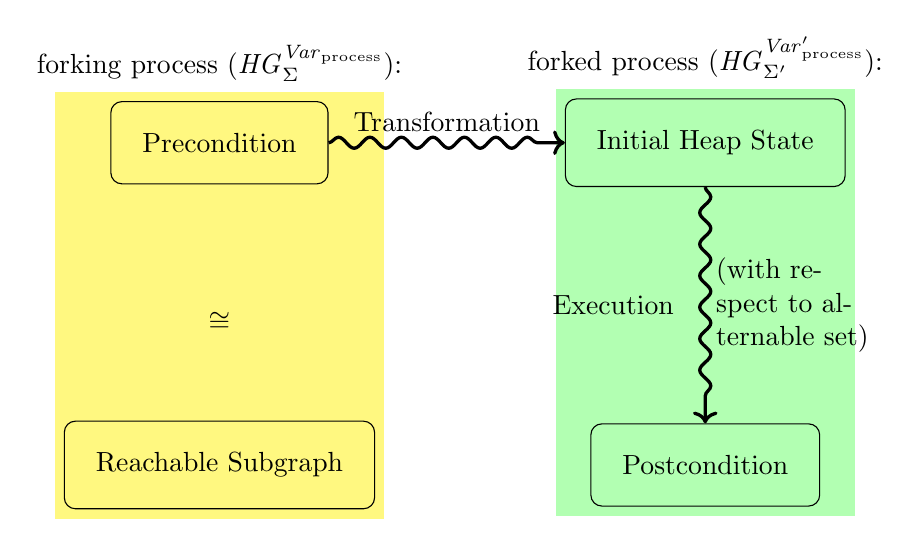
\begin{tikzpicture}[node distance=3cm]
	%states
	\node [textnode] (P) {Precondition};
	\node [textnode, below=of P] (R) {Reachable Subgraph};
	\node [textnode, right=of P] (I) {Initial Heap State};
	\node [textnode] (Q) at (R-|I)   {Postcondition};
	%cong
	\node [below=1.5cm and 1.5cm of P] {$\cong$};

	\begin{scope}[on background layer]
		\node [fill=yellow!50, fit=(P) (R), label={90:forking process ($\HG$):}] {};
		\node [fill=green!30,  fit=(I) (Q), label={90:forked  process ($\mathit{HG}^{\PI'}_{\Sigma'}$):}] {};
	\end{scope}

	%computation
	\draw [very thick,->, decorate,
	decoration={snake,amplitude=.7mm, segment length=4mm, post length=2mm}]
	(I) to node[left, text width=1.8cm]{Execution} node[right, text width=2cm]{(with respect to alternable set)}(Q);
	\draw [very thick,->, decorate,
	decoration={snake,amplitude=.7mm, segment length=4mm, post length=2mm}]
	(P) to node[above]{Transformation} (I);

	
\end{tikzpicture}

		\end{center}
		\caption{Graphical representation of the coherences between precondition,
		initial heap state, reachable subgraph and postcondition}
		\label{fig:forkHeaps}
	\end{figure}
	For every program the set of contracts is formally described as a function
	\begin{equation*}
		\Cont\colon\Proc\rightarrow
		\mathbb{P}(\HG\times\mathbb{P}(E)\times\mathit{HG}_{\Sigma'}^{\PI'})
	\end{equation*}
	where for every program $m$ and every contract $C=(P_C, E_C, Q_C)\in
	\Cont(m)$ holds that $E\subseteq E^{P_C}_{\mathit{WR}}$, thus the set of
	alterable edges ($E_{C}$) is a subset of the edges with write access of the
	precondition. 

	The necessary graph transformations associated with the fork
	statement are examined in the following. Let $H$ be an \emph{\ac{HG}} and
	$C = (P_{C}, E, Q_{C})\in\mathit{Cont}(m)$. Let $\ap_{1},\dots,\ap_{n}$ be
	the nodes that are identified by the actual parameter of the fork statement.
	This means that for the statement
	\begin{lstlisting}
t = fork(m($x_{1},\dots,x_{n}$));
	\end{lstlisting}
	with the current heap representation $H$ it holds that
	$\ap_{i} = \llbracket x_{i}\rrbracket_{H}$ for all $1\leq i\leq n$.
	Thus the set of reachable edges from the actual parameter is defined as
	$\reach(\ap_{1},\dots,\ap_{n})$.
	The actual precondition for the newly forked process is
	the current \emph{heap} representation reduced to the subgraph which is
	induced by the reachable part. This subgraph is defined as follows:
	\begin{definition}[Edge Induced Subgraph]
		Let $H$ be a  \emph{\ac{HG}} and $E'\subseteq E_{H}$ a set of edges. Then
		the \emph{subgraph induced by $E'$} is defined as
		\begin{equation*}
			H\upharpoonright E' = (\bigcup_{e\in E'}\Lbag\con_{H}(e)\Rbag, E',
			\lab\upharpoonright E', \con\upharpoonright E',\ext\upharpoonright E',
			\perm\upharpoonright E')
		\end{equation*}
	\end{definition}
	To find the fitting contract $C$ for the fork statement it is necessary that
	the reachable subgraph forms the precondition of $C$ and the actual
	parameters agree with the formal parameters. Let $\fp_{1},\dots,\fp_{n}$
	denote the nodes of the formal parameters within the precondition of $C$.
	Then the reachable subgraph is structurally identical to the precondition
	and the actual parameters agree with the formal parameters. Let $R$ denote
	the reachable subgraph of a fork statement and $P$ denote the fitting
	precondition. Then $R$ and $P$ are isomorphic and especially this
	isomorphism matches formal and actual parameter. Let $R\afiso P$
	denote the existence of such an isomorphism.

	Once again reconsider the example in Figure \ref{fig:BinTreeProgLangPerm}
	and let
	\begin{equation*}
		C = \left(\parbox{5cm}{\resizebox{5cm}{!}{\input{tikz/precondition}}},
		\{e_2,e_3,e_4, e_7, e_8\},
		\parbox{5cm}{\resizebox{5cm}{!}{\input{tikz/postcondition}}}\right)
	\end{equation*}
	be a possible contract such that $C\in\Cont(\mathit{traverse})$ and $v_1$ is
	the only formal parameter. Here $l$ and $r$ abbreviate $\mathit{left}$ and
	$\mathit{right}$ respectively. Note that $C$ fulfills that the alterable set
	is a subset of the edges with $\mathit{WR}$ permission of the precondition.
	Secondly, in the postcondition only edges have been altered which were part
	of the alterable set (namely $e_3, e_4$). Thirdly, forking by $C$ leads to
	the replacement seen in Figure \ref{fig:BinTreeProgLangPermReplacement}
	because the induced subgraph of $\{e_2,e_3,e_4,e_7,e_8\}$ is replaced. As it
	can be seen in Figure \ref{fig:BinTreeProgLangPermReplacement} the
	replacement is connected to the node that is identified with $v_1$ and
	$v_{\text{null}}$.  This is because $v_1$ represents an object which is part
	of the main process as well as the newly forked one. Such nodes are called
	\emph{border} nodes and are defined as those nodes that are connected to
	edges of the alterable set and to edges that are not part of the alterable
	set. Additionally, the placeholder in Figure
	\ref{fig:BinTreeProgLangPermReplacement} is also
	connected to $v_{\text{null}}$, which is generally assumed for all
	placeholder, thus the heap representation of every process can refer to the
	same distinguishable \textbf{null} value. The formal definition of the set
	of border nodes is closely connected to the definition
	of reachability and is therefore likewise postponed to Section
	\ref{sec:abstractsemantics}. For now the set of
	border nodes for a contract $C$ and a heap representation $H$ is denoted by
	$\border_H(C)$\footnote{just like the reachable set this set is potentially
	a superset of the actual border nodes}. These border nodes represent the
	connection points between the heap representation of the main process and
	the part of the heap of the forked process that can be altered. For joining
	the process later on it is crucial to identify these nodes in the
	postcondition. This is achieved by using the mechanism of \emph{external
	nodes} as introduced for \emph{hyperedge replacement} in Section
	\ref{sec:hyperedgereplacement}.
	With these considerations in mind the transformation of the heap
	representation that models the fork statement can be described.
	Let therefore
	\begin{itemize}
		\item $t$ = \textbf{fork}($m(x_1,\dots,x_n)$);
		\item with $H$ as the current heap representation,
		\item $\ap_{i} = \llbracket x_{i}\rrbracket_{H}$ for all $1\leq i\leq n$,
		\item $(P_{C},E_{C},Q_{C})\in\Cont(m)$,
		\item $P_{C}\afiso (H\upharpoonright \reach(\ap_{1},\dots,\ap_{n}))$,
		\item $t\in\PI$,
		\item $b_{C}(H)$ denote the set of border nodes,
		\item $\enum_{b_{C}(H)} =
			\enum_{b_{C}(H)}(1)\dots\enum_{b_{C}(H)}(|b_{C}(H)|)$ is an arbitrary
			sequence of the border nodes
	\end{itemize}
	W. l. o. g. it is assumed that $P_C$ shares nodes and edges with $H$ which
	can easily achieved by renaming the edges and nodes of $P_C$ according to
	the existing isomorphism. Then the graph transformation can be given as
	follows:
	\begin{equation*}
		\label{eq:H'}
		H' = \underbrace{\overbrace{\underbrace{
		\overbrace{H[\downarrow t]}^{\circled{1}}[\setminus E_{C}]}_{\circled{2}}
		[+_{\mathit{WR}}N_{\{t\}}\rightrightarrows
		\enum_{b_{C}(H)}]}^{\circled{3}}[(E_{P}\setminus E_{C})-\{t\}]}_{
		\circled{4}}
	\end{equation*}
	where the different steps state the following:
	\begin{enumerate}[label=\protect\circled{\arabic*}]
		\item the process identifier used for the newly forked process is freed
		\item the edges that the forked process demands write access on are
			removed from the heap representation
		\item the formerly removed edges are replaced with an hyperedge
		\item to all edges that can be read by the newly forked process the
			appropiate token is added
	\end{enumerate}
	Formally this process is therefore described by the following transition
	rule:
	\begin{prooftree}
		\label{prooftree:fork}
		\AxiomC{$(P_{C}, E_{C}, Q_{C})\in\mathit{Cont}(m)$}
		\AxiomC{$P_{C}\afiso (H\upharpoonright \reach
		(\llbracket p_{1}\rrbracket_{H},\dots,\llbracket p_{n}\rrbracket_{H}))$}
		\BinaryInfC{$(t = \text{fork}(m(p_1,\dots,p_n)), H)\rhd
			(\varepsilon, H')$}
	\end{prooftree}

	For the \emph{join} statement some formalisms of \emph{\aclp*{HRG}}, namely
	\emph{\acl*{HR}} is used and therefore the definition is postponed and
	\acl*{HR} is introduced before.

\subsection{Hyperedge Replacement}
\label{sec:hyperedgereplacement}
	In the following the concept of \emph{\ac{HR}} is presented.
	\emph{\Ac{HR}} is a  graph transformations which replaces single hyperedges
	by more complex graphs \cite[p. 104]{HandbookGraphGrammars}. As the fork
	statement replaces parts of the heap by a single hyperedge in order to
	\enquote{hide} this subgraph, rendering it unavailable for the main process.
	Indeed the \enquote{hidden} subgraph still exists within the heap
	representation of the forked process and can especially be returned by a
	\emph{join} statement. Therefore a way to re-integrate this subgraph is
	discussed in the following. A possible way to present rules for substituting
	hyperedges by hypergraphs are \emph{production rules} which have the form
	$p\colon X\rightarrow H$. Here $X$ is a label and $H$ a hypergraph and this
	production rule $p$ can be applied to a hypergraph by removing a
	$X$-labeled edge and replacing it by the hypergraph $H$. For better
	understanding the production rule in Figure \ref{fig:productionrule} is
	considered in the following. On the right hand side of this production rule
	the nodes marked by $1$ and $2$ are \emph{external nodes} of the hypergraph
	and their annotation is their position in the sequence $\ext$. For the
	hyperedges that are labeled with $B$ the numbers denote the position of the
	nodes in the sequence of connected nodes.
	\begin{figure}[ht!]
		\begin{center}
			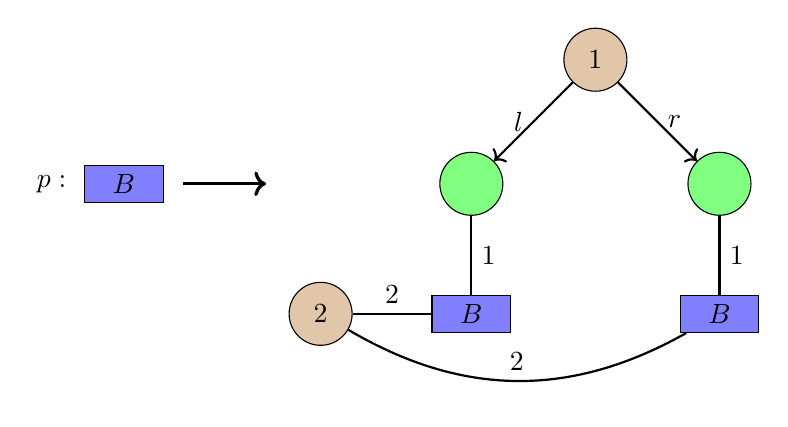
\begin{tikzpicture}
	\node (p) {$p:$};
	\node[he, right=0.1cm of p] (lhs) {$B$};
	\node[node, right=3.5cm of lhs] (v2) {};
	\node[node, above right=of v2, ext] (v1) {1};
	\node[node, below right=of v1] (v3) {};
	\node[he, below=of v2] (e1) {$B$};
	\node[he, below=of v3] (e2) {$B$};
	\node[node, left=of e1, ext] (v4) {2};

	\draw[very thick, ->, shorten >=2.2cm, shorten <=7pt] (lhs) to (v2);
	\draw[sel] (v1) to node[left ]{$l$} (v2);
	\draw[sel] (v1) to node[right]{$r$} (v3);
	\draw[connector] (e1) to node[right]{1} (v2);
	\draw[connector] (e1) to node[above]{2} (v4);
	\draw[connector, bend left] (e2) to node[above]{2} (v4);
	\draw[connector] (e2) to node[right]{1} (v3);
\end{tikzpicture}

			\caption{A possible production (permissions are omitted)}
			\label{fig:productionrule}
		\end{center}
	\end{figure}
	In order to replace for instance such a $B$-labeled hyperedge in an
	\emph{\ac{HG}} the external nodes of the right hand side of the production
	rule are identified with the nodes connected to the hyperedge. A simple
	example (see Figure \ref{fig:replacement}) illustrates such a replacement.
	Note that the external nodes and the connected nodes that are identified
	had the same position within the respective sequences.
	\begin{figure}
		\begin{center}
			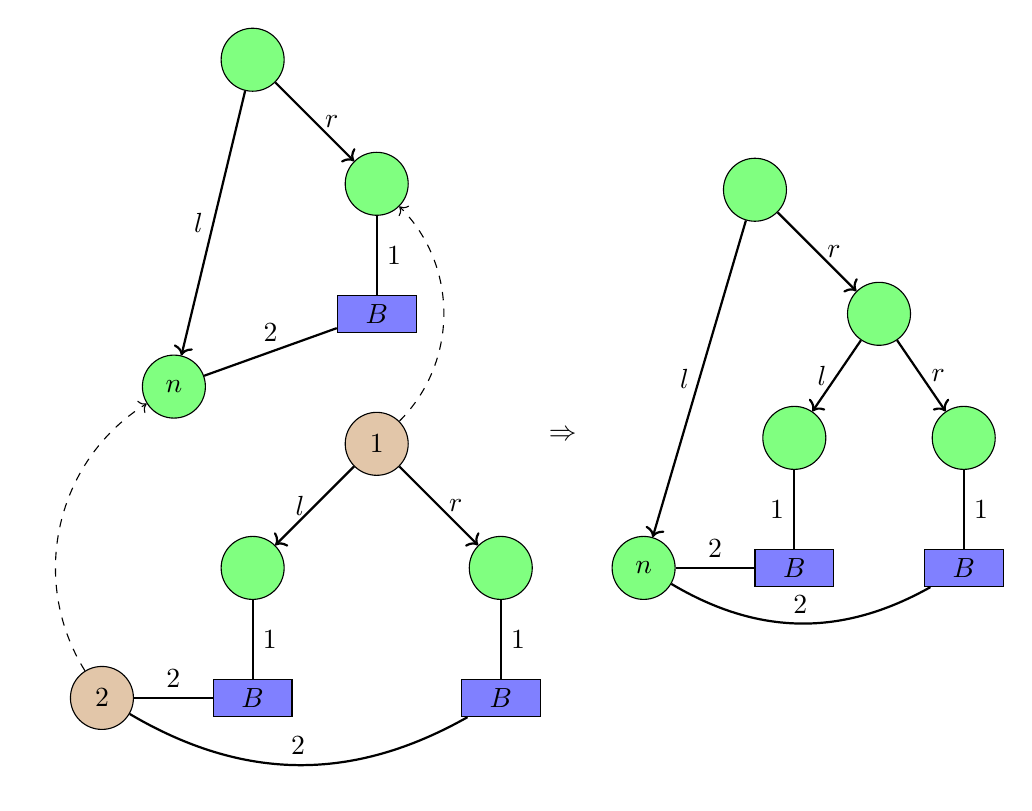
\begin{tikzpicture}
	%graph
	\node[node] (s1) {};
	\node[node, below right=of s1] (s3) {};
	\node[node, node distance=2 and 2, below left =of s3] (s2) {$n$};
	\node[he, below=of s3] (e3) {$B$};

	\draw[sel] (s1) to node[left ]{$l$} (s2);
	\draw[sel] (s1) to node[right]{$r$} (s3);
	\draw[connector] (e3) to node[above]{2} (s2);
	\draw[connector] (e3) to node[right]{1} (s3);

	%rhs of production rule:
	\node[node, below=of e3, ext] (v1) {1};
	\node[node, below left=of v1] (v2) {};
	\node[node, below right=of v1] (v3) {};
	\node[he, below=of v2] (e1) {$B$};
	\node[he, below=of v3] (e2) {$B$};
	\node[node, left=of e1, ext] (v4) {2};

	\draw[sel] (v1) to node[left ]{$l$} (v2);
	\draw[sel] (v1) to node[right]{$r$} (v3);
	\draw[connector] (e1) to node[right]{1} (v2);
	\draw[connector] (e1) to node[above]{2} (v4);
	\draw[connector, bend left] (e2) to node[above]{2} (v4);
	\draw[connector] (e2) to node[right]{1} (v3);

	%connection
	\draw[dashed, ->, bend right=45] (v1) to (s3);
	\draw[dashed, ->, bend left=45]  (v4) to (s2);

	%leadsto symbol
	\node[above right=1.2cm and 0.2cm of v3] {$\Rightarrow$};

	%result
	\node[node] (null) [right=of v3] {$n$};
	\node[he] (e1) [right=of null] {$B$};
	\node[node, above=of e1] (root-right-left) {};
	\node[node, above right=1cm and 0.5cm of root-right-left](root-right){};
	\node[node, below right=1cm and 0.5cm of root-right](root-right-right){};
	\node[node, above left=of root-right] (root) {};
	\node[he, below=of root-right-right] (e2) {$B$};

	\draw[sel] (root) to node[right]{$r$} (root-right);
	\draw[sel] (root) to node[left ]{$l$} (null);
	\draw[sel] (root-right) to node[left ]{$l$} (root-right-left);
	\draw[sel] (root-right) to node[right]{$r$} (root-right-right);
	\draw[connector] (e1) to node[left ]{1} (root-right-left);
	\draw[connector] (e2) to node[right]{1} (root-right-right);
	\draw[connector] (e1) to node[above]{2} (null);
	\draw[connector, bend left] (e2) to node[above]{2} (null);

\end{tikzpicture}

			\caption{Illustration of an \acl{HR}}
			\label{fig:replacement}
		\end{center}
	\end{figure}
	Such a replacement of an hyperedge is called a \emph{derivation} and is
	formally described as follows:
	\begin{definition}[Hyperedge Replacement]
		Let $p$ be a production rule of the form $p\colon X\rightarrow K$,
		$H\in\mathit{HG}_{\Sigma}$ a \emph{\ac{HG}} with an edge $e\in E_{H}$
		with $\mathit{lab}_{H}(e)=X$ and $|\ext_K| = |\con_{H}(e)|$. Then
		$H' = H[e/K]$ is an \emph{\ac{HG}} with:
		\begin{itemize}
			\item $V_{H'}=V_{H}\cup(V_{K}\setminus\Lbag \mathit{ext}_{K}\Rbag)$
			\item $E_{H'}=(E_{H}\setminus\{e\})\cup E_K$
			\item $\begin{aligned}
				\mathit{con}_{H'}=\mathit{con}_{H}\upharpoonright(E_{H} \setminus
				\{e\})\cup((\mathit{id}_{K}&[\ext_{K}(1)\mapsto\con_{H} (e)(1)]
				\dots\\
					&[\ext_{K}(|\ext_{K}|)\mapsto\con_{H}(e)(|\ext_{K}|)])\circ
				\mathit{con}_{K})
			\end{aligned}$
			\item $\mathit{lab}_{H'}=\mathit{lab}_{H}\upharpoonright(E_{H}
				\setminus\{e\})\cup\mathit{lab}_{K}$
			\item $\mathit{ext}_{H'}=\mathit{ext}_{H}$
			\item $\mathit{perm}_{H'}=\mathit{perm}_{H}\upharpoonright(E_{H}
				\setminus\{e\})\cup \mathit{perm}_{K}$
		\end{itemize}
	\end{definition}
	An \emph{\ac{HG}} $H'$ is derived from an \emph{\ac{HG}} $H$ by a production
	rule $p\colon X\rightarrow K$ (denoted by $H\xRightarrow{p}H'$) if $H'$ is
	isomorphic to $H[e/K]$ for any edge $e$ labeled with $X$. Furthermore
	$\Rightarrow^{\ast}$ is the transitive closure of this relation.
	\subsection{Join}
	\label{sec:join}
	Having introduced the mechanism of hyperedge replacement the postponed
	semantics of the join statement can now be addressed. Therefore
	it is distinguished between the \emph{joining} process which is the one
	actually executing the join statement and the \emph{joined} process
	which is the one that terminated and now returns its permissions.
	Returning this permissions can be done in two separate steps:
	Firstly, the permissions for the shared edges, i.e. those edges which
	$\mathit{BasePerm}$ is either $\mathit{RD}$ or $\mathit{RD^{\ast}}$ for the
	joined process, are returned.
	Since these edges are still present in the heap representation of the
	joining process returning those permissions is a
	matter of mutating the \emph{\ac{PE}} of the heap representation of
	the joining process. Secondly, the edges which were allowed to be
	altered are returned, i.e. edges which $\mathit{BasePerm}$ is either
	$\mathit{WR}$ or $\mathit{WR^{\ast}}$. This is done by replacing the
	hyperedge in the joining process which represents this part of the
	heap by its corresponding \emph{\ac{HG}} of the joined
	process. This imposes a further restriction to the contracts which have to
	ensure that the external nodes of the postcondition of the forked process
	are the same as the border nodes of the placeholder in the heap
	representation of the forking process. To do so, the sequence of external
	nodes in the precondition is used to encode which nodes are border nodes
	and the isomorphism $\afiso$ is restricted to map the border nodes in the
	heap representation of the forking process to the external nodes in the
	precondition. Following it is formally described how the initial heap state
	for the forked process is obtained from the contract
	$C = (P_C, E_C, Q_C)$:\footnote{which refers to the \emph{transformation} in
	Figure \ref{fig:forkHeaps}}
	Let $\ap_{1},\dots,\ap_{n}$ denote the nodes that mark the actual parameters
	and $\fp_{1},\dots,\fp_{1}$ denote the names of the formal paramters they
	are matched to (especially $\fp_{i}\in\Sigma'$ for all $1\leq i\leq n$).
	Furthermore let for all $s\in\Sel$ $s'\in\Sel'$ denote the corresponding
	selector used to describe the heap states of forked processes,
	then $I \in\mathit{HG}^{\PI'}_{\Sigma'}$ is the initial heap state for the
	forked process with:
	\begin{itemize}
		\item $V_I = \{v^{I}_{v'} \mid v'\in V_{P_{C}}\}$
		\item $E_I = \{e^{I}_{e'} \mid e'\in E_{P_{C}}\} \cup
			\{e_{\fp_i}\mid 1\leq i\leq n\}\cup\{e_{v}\mid v\in(\Var'\setminus
			\{\fp_{i}\mid 1\leq i\leq n\})\}$
		\item $\con_{I} = \{v'\mapsto v^{I}_{v'}\mid v'\in V_{P_{C}}\}
			\circ\con_{P_{C}}\cup \{e_{\fp_i}\mapsto\ap_i\mid 1\leq i\leq n\}
			\cup\{e_{v}\mapsto v_{\text{null}}\mid v\in(\Var'\setminus
			\{\fp_{i}\mid 1\leq i\leq n\})\}$
		\item $\lab_{I} = \{e_{\fp_{i}}\mapsto\fp_{i}\mid 1\leq i\leq n\}
			\cup\{e\mapsto s'\mid\lab_{P_{C}}(e) = s\}\cup\{e_{v}\mapsto v\mid
			v\in(\Var'\setminus \{\fp_{i}\mid 1\leq i\leq n\})\}$
		\item $\ext_I = \{v^{I}_{v'}\mapsto v'\mid v'\in V_{P_{C}}\}
			(\enum_{\border_{P_C}}(1)\dots\enum_{\border_{P_C}}(|\border_{P_{C}}
			(C)|))$
		\item $\perm_{I} = \{e\mapsto\mathit{WR}\mid e\in E_{C}\}\cup
			\{e\mapsto\mathit{RD}\mid e\in E_{P_{C}}\setminus E_{C}\}\cup
			\{e_{v}\mapsto\mathit{WR}\mid v\in(\Var'\setminus \{\fp_{i}\mid 1\leq
				i\leq n\})$
	\end{itemize}
	Note that actually only the selectors are renamed and variables introduced
	for the formal parameters that point to the nodes the actual parameters
	pointed to in the fork statement, also all other variables of $\Var'$ are
	introduced and initially point to $v_{\text{null}}$. Furthermore the
	external nodes of the
	initial heap state are used to mark the border nodes in order to ensure that
	the \enquote{$\mathit{WR}$-part} of the postcondition agrees on the shared
	objects when it is joined. At last, all permissions in the initial heap
	state are simple and grant those access tickets that the contract demands.
	From this initial heap state the execution of the forked program starts.

	For both steps of returning permissions for the join statement it is
	important to determine if all
	permissions are returned which were derived when the process was forked.
	This is not the case for all edges which \emph{\acp{PE}} are not
	\emph{simple} or which $\mathit{BasePerm}$ is \enquote{starred} (thus
	$\mathit{WR^\ast}$ or $\mathit{RD^\ast}$). These permissions are
	unrecoverably lost and this propagates strictly to the permissions of the
	heap representation of the joining process.
	
	For returning the read permissions it is avoided to match the
	edges from the heap representation of the joining and
	joined process since it imposes further difficulties later on.
	Therefore the minimal permission is returned: for all
	edges of the joining process from which permissions were 
	derived to the joined process the $\mathit{BasePerm}$ is 
	\enquote{starred} if there is \emph{any} edge in the postcondition
	for which the permission cannot be completely returned.

	Returning the write permissions is done by simply applying a
	production rule to the hyperedge of the joining process that
	represents the borrowed part. Let now
	$C = (P_{C}, E_{C}, Q_{C})\in\Cont(m)$ be the contract by which
	the joined process was forked (note that this contract has to be the same
	as for the fork statement that created the process which is re-joined now,
	in order to save the contract for matching it from fork to join statement
	it can be e. g. attached to the placeholder) and $T_t$ the set of all
	aliases of the process identifier $t$ that is used in the join statement.
	Further the following few definitions are used for convenience:
	\begin{equation*}
		\label{eq:joinH}
		Q'_{1}=Q_{C}[\downarrow\mathit{enum}_{\mathit{Var}'_{\text{thread}}}(1)]
		\dots[\downarrow\mathit{Var}'_{\text{thread}}
		(|\mathit{Var}'_{\text{thread}}|)]
	\end{equation*}
	Note that for $Q'_{1}$ all \emph{\ac{PE}} are \emph{simple} and every not
	yet returned permission caused the $\mathit{BasePerm}$ to be
	\enquote{starred}.
	\begin{equation*}
		Q'_{2} = Q'_{1}[\setminus (E^{Q'_{1}}_{\mathit{RD}}\cup
			E^{Q'_{1}}_{\mathit{RD^{\ast}}})]
	\end{equation*}
	$Q'_{2}$ represents the state where the heap representation of the
	joined process is reduced to the edges of the alterable set.
	Now two transition rules are used to model the semantics of the join
	statement where the first one describes the case with lost read
	permissions and the second one describes the case where all
	read permissions can be completely returned:
	\begin{prooftree}
		\label{prooftree:join}
		\AxiomC{$E^{Q'_{1}}_{\mathit{RD*}}\neq\emptyset$}
		\AxiomC{$H[\downarrow T_{t}]\xRightarrow{N_{T_{t}}\rightarrow Q'_{2}}H'$}
		\BinaryInfC{$(\text{join}(t), H)\rhd(\varepsilon,H')$}
	\end{prooftree}
	Note that $H[\downarrow T_{t}]$ is used which successively drops the process
	identifier in the token $T_{t}$
	\begin{equation*}
		\text{\enquote{$H[\downarrow T_{t}] = H[\downarrow\enum_{T_{t}}(1)]\dots
		[\downarrow\enum_{T_{t}}(|T_{t}|)]$}}
	\end{equation*}
	but preserves $N_{T_{t}}$ in order to replace it by the given production
	rule.
	\begin{prooftree}
		\AxiomC{$E^{H'_{1}}_{\mathit{RD*}}=\emptyset$}
		\AxiomC{$H[\leftarrow T_{t}]\xRightarrow{N_{T_{t}}\rightarrow Q'_{2}}H'$}
		\BinaryInfC{$(\text{join}(t), H)\rhd(\varepsilon,H')$}
	\end{prooftree}
	This concludes the modelling of the semantics of the presented programming
	language and in the following it is dealt with abstraction techniques to
	approach potentially unbounded structures.

\newpage
\section{Concretisation \& Abstraction}
	Making use of dynamic allocation and deallocation can lead to heap
	structures of unbounded size. In order to present these structures in a
	finite manner \emph{\ac{HR}} can be used in order to concretise and abstract
	heap states by applying production rules for concretisation and by applying
	production rules backwards for abstraction. Therefore introduce a set of
	production rules in order to abstract parts of the heap representation.
	In order to illustrate the
	following steps the data structure of binary trees is examined along the
	definitions\footnote{this example reassembles the \emph{\acl*{HRG}} from
	\cite[p. 21]{fmsd}}. Reconsider the structure in the example from Figure
	\ref{fig:BinTreeProgLang} and furthermore the \emph{\ac{HR}} from Figure
	\ref{fig:replacement}. When the node marked by $n$ is interpreted as
	$v_{\text{null}}$ and the production rule from Figure
	\ref{fig:productionrule} is applied repetitively arbitrary large binary
	trees can be constructed. But it is already noteable that repetitive
	application of this production rule always leads to further $B$-labeled
	edges. The following formal introduction of the concept of abstraction
	follows mostly \cites{fmsd}{InductivePredicates}{LocalGreibachNormalForm}.

	In order to distinguish the hyperedges that are used for the abstract
	representation of a subgraph from the hyperedges that represent
	placeholders, selectors or variables a new set of so called
	\emph{nonterminals} $N$ is introduced. For the above considered example of
	binary trees this set would be $N=\{B\}$. In the following
	$\Sigma_{N} = \Sigma\biguplus N$ denotes the set of labels for
	\emph{\acp{HG}} that are partially concrete and partially abstract.
	Furthermore these \emph{nonterminals} are expected to connect always the
	same amount of nodes. This amount is called the rank of the nonterminal.
	Therefore a function $\rk\colon N\rightarrow \mathbb{N}$ is given and for
	every \emph{\ac{HG}} $H$ it holds that if $\lab_{H}(e)\in N$ then
	$|\con_{H}(e)|=\rk(\lab_{H}(e))$, the rank of $B$ for example is $2$.
	The set of all these partially abstract \emph{\acp{HG}} is denoted by $\HGN$
	and the set of \emph{\acp{HG}} that furthermore satisfy the restrictions of
	\emph{\acp{HC}} is denoted by $\HCN$. Note that for now the permissions were
	neglected but are actually incorporated as follows: a production rule
	$p\colon X\rightarrow H$ with $X\in N$ is annotated by
	a permission $\rho$ ($p_{\rho}$) such that for
	$p_{\rho}\colon X\rightarrow H$
	holds that $\img(\perm_{H}) = \{\rho\}$ (thus all edges in $H$ hold
	permission $\rho$). Furthermore this production rule must only be applied to
	an $X$-labeled edge if this edge holds the permission $\rho$.

	\subsection{Hyperedge Replacement Grammar}
	To apply abstraction and concretisation a set of production rules is used.
	Such a set of production rules is called a \emph{\ac{HRG}}. Formally defined
	as follows:
	\begin{definition}[Hyperedge Replacement Grammar]
		A \emph{\acl{HRG}} over an alphabet $\Sigma_N$ and
		$\PI$ is a finite set of
		production rules of the form $p_{\rho}\colon X\rightarrow G$ where
		$X\in N$, $\rho\in\mathit{PES}_{\PI}$,
		$G\in\mathit{HG}_{\Sigma_{N}}$ and $\rk(X) = |\ext_{G}|$.
	\end{definition}
	$\HRG$ denotes the set of all \emph{\acp{HRG}} over $\Sigma_{N}$ and
	$\PI$. Especially, in this paper the concepts of structural abstraction and
	permission accounting are independently examined, this means in order to
	separate those concepts the following definition is used which states that
	every production rule is available for every permission:
	\begin{definition}[Fully Permissive Grammar]
		\label{def:fpg}
		$G\in\HRG$ is called \emph{fully permissive} if the following holds:
		Every production rule $p\colon X\rightarrow H$ in $G$ exists for every
		$\rho\in\PES$.
	\end{definition}
	The set of all \emph{\acp{fpHRG}} is denoted by $\fpHRG$.

	In the following some definitions regarding \emph{\acp{fpHRG}} are
	introduced. These intuitions and their respective definitions are examined
	in their structural concepts only since the incorporation of permissions is
	straightforward:
	\begin{itemize}
		\item For $G\in\fpHRG$ $G^{X} = \{ X'\rightarrow H\in G \mid X'=X\}$
			denotes the set of all production rules for a nonterminal $X$.
		\item For a production rule $p\colon X\rightarrow H$ $\lhs(p)$ is used
			for $X$ and respectively $\rhs(p)$ for the right hand side $H$. $\rhs$
			and $\lhs$ are lifted to sets of \emph{production rules} by
			elementwise application.
		\item The \emph{handle} of a nonterminal is introduced which is
			the \emph{\ac{HG}} that contains one edge labeled by the nonterminal
			and nodes connected to this nonterminal. Formally:
				\begin{definition}[Handle]
					For a \emph{\ac{fpHRG}} $G\in\fpHRG$ and a nonterminal $X\in N$
					the \emph{handle} of $X$ is the \emph{\ac{HG}} $X^{\bullet}
					\in\mathit{HG}_{\Sigma_{N}}$
					with:
					\begin{itemize}
						\item $V_{X^{\bullet}} = \{v_1,\dots,v_{\mathit{rk}(X)}\}$
						\item $E_{X^{\bullet}} = \{e\}$
						\item $\mathit{con}_{X^{\bullet}} =
							\{e\mapsto v_1\cdots v_{\mathit{rk}(X)}\}$
						\item $\mathit{lab}_{X^{\bullet}} =
							\{e\mapsto X\}$
						\item $\mathit{ext}_{X^{\bullet}} = \epsilon$
						\item $\mathit{perm}_{X^{\bullet}} = \{e\mapsto\rho\}$
					\end{itemize}
				\end{definition}
		\item For hyperedges labeled with nonterminals the position on
			which a node is attached on is called a \emph{tentacle}. A
			tentacle is just a label and the position a node is attached to an
			edge of this label.
				\begin{definition}[Tentacle]
					A \emph{tentacle} is a pair $(X,i)$ where $X\in N$ and
					$i\in\{1,\dots \mathit{rk}(X)\}$.
				\end{definition}
		\item For hyperedges labeled with nonterminals the notion of
			tentacles can be extended in order to describe how two nodes are
			connected by this hyperedge. Such a connection is called a
			\emph{bridge} and reassembles two tentacles of the same nonterminal.
				\begin{definition}[Bridge]
					A \emph{bridge} is a triple $(i, X, j)$ where $X\in N$ and
					$1\leq i,j\leq \rk(X)$.
				\end{definition}
			Let $\br(S)$ denote the set of all bridges for the set of ranked
			labels $S$.
	\end{itemize}
	Consider the following possible \emph{\ac{fpHRG}} $G$ which describes the
	abstraction of binary trees:
	\begin{equation*}
		\label{eq:G}
		G = \left\{\begin{aligned}
			 & \parbox{5cm}{\resizebox{5cm}{!}{
					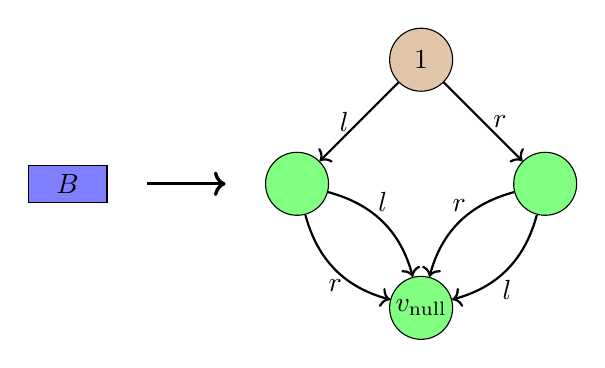
\begin{tikzpicture}
	\node[he] (lhs) {$B$};
	\node[node, right=1cm and 2cm of lhs] (v2) {};
	\node[node, ext, above right=of v2] (v1) {$1$};
	\node[node, below right=of v1] (v3) {};
	\node[node, below right=of v2] (null) {$v_{\text{null}}$};

	\draw[very thick, ->, shorten >=0.5cm, shorten <=0.5cm] (lhs) to (v2);
	\draw[sel] (v1) to node[left] {$l$} (v2);
	\draw[sel] (v1) to node[right]{$r$} (v3);
	\draw[sel, bend left] (v2) to node[above]{$l$} (null);
	\draw[sel, bend right] (v2) to node[below]{$r$} (null);
	\draw[sel, bend left] (v3) to node[below]{$l$} (null);
	\draw[sel, bend right] (v3) to node[above]{$r$} (null);
\end{tikzpicture}

				}}, \parbox{5cm}{\resizebox{5cm}{!}{
					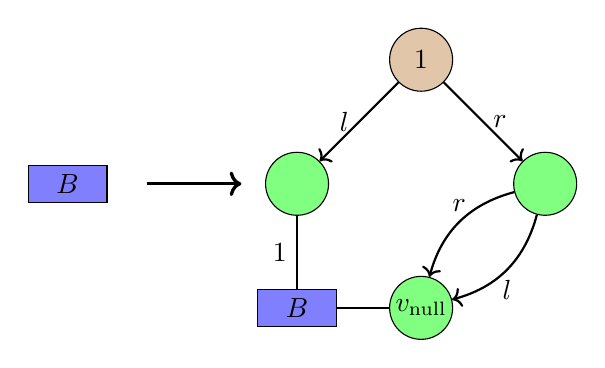
\begin{tikzpicture}
	\node[he] (lhs) {$B$};
	\node[node, right=1cm and 2cm of lhs] (v2) {};
	\node[node, ext, above right=of v2] (v1) {$1$};
	\node[node, below right=of v1] (v3) {};
	\node[node, below right=of v2] (null) {$v_{\text{null}}$};
	\node[he] (e1) at (null-|v2) {$B$};

	\draw[very thick, ->, shorten >=0.3cm, shorten <=0.5cm] (lhs) to (v2);
	\draw[sel] (v1) to node[left] {$l$} (v2);
	\draw[sel] (v1) to node[right]{$r$} (v3);
	\draw[connector] (v2) to node[left]{$1$} (e1);
	\draw[sel, bend left] (v3) to node[below]{$l$} (null);
	\draw[sel, bend right] (v3) to node[above]{$r$} (null);
	\draw[connector] (e1) to (null);
\end{tikzpicture}

				}},\\& \parbox{5cm}{\resizebox{5cm}{!}{
					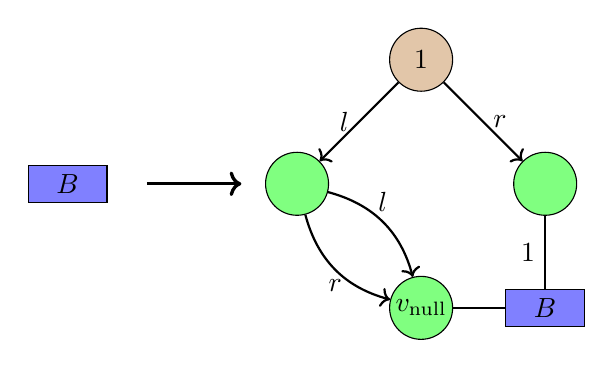
\begin{tikzpicture}
	\node[he] (lhs) {$B$};
	\node[node, right=1cm and 2cm of lhs] (v2) {};
	\node[node, ext, above right=of v2] (v1) {$1$};
	\node[node, below right=of v1] (v3) {};
	\node[node, below right=of v2] (null) {$v_{\text{null}}$};
	\node[he] (e1) at (null-|v3) {$B$};

	\draw[very thick, ->, shorten >=0.3cm, shorten <=0.5cm] (lhs) to (v2);
	\draw[sel] (v1) to node[left] {$l$} (v2);
	\draw[sel] (v1) to node[right]{$r$} (v3);
	\draw[connector] (v3) to node[left]{$1$} (e1);
	\draw[sel, bend left] (v2) to node[above]{$l$} (null);
	\draw[sel, bend right] (v2) to node[below]{$r$} (null);
	\draw[connector] (e1) to (null);
\end{tikzpicture}

				}}, \parbox{5cm}{\resizebox{5cm}{!}{
					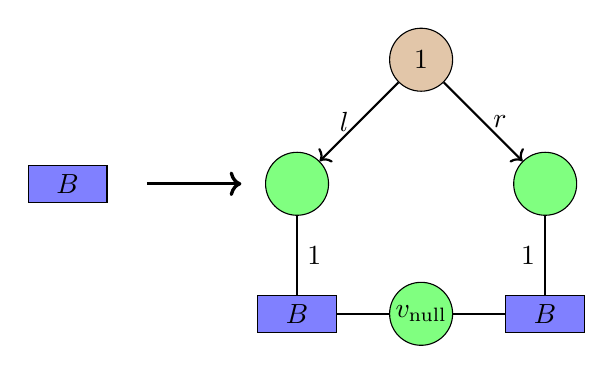
\begin{tikzpicture}
	\node[he] (lhs) {$B$};
	\node[node, right=1cm and 2cm of lhs] (v2) {};
	\node[node, ext, above right=of v2] (v1) {$1$};
	\node[node, below right=of v1] (v3) {};
	\node[he, below=of v3] (e2) {$B$};
	\node[he, below=of v2] (e1) {$B$};
	\node[node] (null) at (e1-|v1) {$v_{\text{null}}$};

	\draw[very thick, ->, shorten >=0.3cm, shorten <=0.5cm] (lhs) to (v2);
	\draw[sel] (v1) to node[left] {$l$} (v2);
	\draw[sel] (v1) to node[right]{$r$} (v3);
	\draw[connector] (v3) to node[left]{$1$} (e2);
	\draw[connector] (v2) to node[right]{$1$} (e1);
	\draw[connector] (e1) to (null);
	\draw[connector] (e2) to (null);
\end{tikzpicture}

		}}
		\end{aligned} \right\}
	\end{equation*}
	Note that these production rules are present for every permission, since it
	is a fully permissive \emph{\ac{HRG}} and that from $H\in\HGN$ it can be
	possible to derive multiple \emph{\acp{HG}} since there might be
	more than one production rule for any nonterminal. Consider
	therefore the \emph{\ac{HG}} of Figure \ref{fig:replacement} and the
	\emph{\ac{fpHRG}} $G$ from above. It is easily to see that multiple
	different \emph{\acp{HG}} can be derived. The set of all these deriveable
	\emph{\acp{HG}} which no longer contain a nonterminal (like the terminal
	words of a string grammar) is called the language of $H$ and defined as
	follows:
	\begin{definition}[Language of an \ac{HG}]
		For $G\in\fpHRG$ and $H\in\mathit{HG}_{\Sigma_{N}}$
		\begin{equation*}
			L_{G}(H) = \{K\in\mathit{HG}_{\Sigma} \mid H \Rightarrow^{*} K\}
		\end{equation*}
		is the \emph{language} from the \emph{\ac{HG}} $H$
		(under the \emph{\ac{fpHRG}} $G$).
	\end{definition}

	\subsection{Properties}
	In the following some properties of \emph{\acp{HRG}} are discussed. The
	presented properties as well as the presented results for \emph{\acp{fpHRG}}
	follow from \cite{LocalGreibachNormalForm}. Actually the design of the
	definitions are built around those in \cite{LocalGreibachNormalForm} to
	focus on the compatibility of adding permissions to the already established
	results. At first it is discussed which selectors a nonterminal actually
	abstracts. By considering the example in Figure \ref{fig:replacement} it can
	easily be seen, that at the different connected nodes of the $B$-labeled
	edge different selectors are abstracted. At the node on the tentacle $(B,1)$
	both selectors $l$ and $r$ are \enquote{hidden} in the abstraction of the
	hyperedge whereas the node on tentacle $(B,2)$ identifies $v_{\text{null}}$
	which must not have any outgoing selectors. This illustrates that different
	selectors can be abstracted at different tentacles. \emph{Typedness} is
	introduced to ensure that application production rules reveals the same
	selectors for every tentacle. The function $\type$ maps from tentacles to
	the sets of the selectors this tentacle abstracts. In the \emph{\ac{fpHRG}}
	from page \pageref{eq:G} it holds that $\type(B,1) = \{l,r\}$. The formal
	definition is as follows:
	\begin{definition}[Typedness]
		For $G\in\fpHRG$ a nonterminal $X\in N$ is called typed if for all
		tentacles $(X,i)$ there is a set $\type(X,i)\subseteq\Sel$ such that for
		all $H\in L_{G}(X^{\bullet})$ where $v^{\bullet}_{i}$ is the node of the
		tentacle $(X,i)$ in $X^{\bullet}$ it holds:
		\begin{equation*}
			\type(X,i) = \lab_H(\out_{H}(v^{\bullet}_{i}))
		\end{equation*}
	\end{definition}
	Note that $\out_{H}(v) = \{e \in E_{H}\mid \con_{H}(1) = v
	\land \lab_{H}(e)\in\Sel\}$ is the set of all outgoing
	selectors from the object represented by $v$. Since different tentacles
	might have different types but the definition
	of \emph{\ac{HC}} enforces that every node is universally typed it is
	possible that the nodes of a handle violate this typing. Therefore the
	notion of handles is expanded to ensure that at least the initial nodes of
	the handle are universally typed:
	\begin{definition}[Typed Handle]
		For a typed nonterminal $X\in N$ let $\mathit{Type} =
		\bigcup_{1\leq i\leq\rk(X)}\type(X,i)$ denote the set of all selectors of
		the nonterminal. The typed handle of $X$ (denoted as $X^{\circ}$) is
		defined as follows:
		\begin{itemize}
			\item $V_{X^{\circ}} = \{v_{1},\dots,v_{\rk(X)},v_{\text{null}}
				\}$
			\item $E_{X^{\circ}} = \{e\} \uplus \{e_{s,i}\mid 1\leq i\leq
				\rk(X), s\in\mathit{Type}\setminus\type(X,i)\}$
			\item $\con_{X^{\circ}} = \{e\mapsto v_{1}\cdots v_{\rk(X)}\}
				\uplus\{e_{s,i}\mapsto v_{i}v_{\text{null}}\mid e_{s,i}\in
				E_{X^{\circ}}\}$
			\item $\lab_{X^{\circ}} = \{e\mapsto X\}\uplus\{e_{s,i}\mapsto s
				\mid e_{s,i}\in E_{X^{\circ}}\}$
			\item $\ext_{X^{\circ}} = \varepsilon$
			\item $\perm_{X^{\circ}} = \{e\mapsto\mathit{WR}\mid e\in
				E_{X^{\circ}}\}$
		\end{itemize}
	\end{definition}

	Secondly, \emph{productivity} is examined which simply states that at
	least one terminal \emph{\ac{HG}} can be derived from this nonterminal.
	Formally stated as:
	\begin{definition}[Productivity]
		For $G\in\HRG$ a nonterminal $X\in N$ is called \emph{productive} if
		\begin{equation*}
			L_{G}(X^{\bullet})\neq\emptyset
		\end{equation*}
		$G$ is called \emph{productive} if all nonterminals in $G$ are
		\emph{productive}.
	\end{definition}

	Following \emph{increasingess} is introduced. The idea is that every right
	hand side of a production rule is strictly \enquote{bigger} than the left
	hand side. Where \enquote{bigger} refers to the number of edges, but also
	terminal \emph{\acp{HG}} are considered \enquote{bigger}. This ensures that
	applying succesively production rules in a backward fashion terminates,
	since every applied production rules reduces the size of the \emph{\ac{HG}}.
	\begin{definition}[Increasingess]
		For $G\in\fpHRG$ a production rule $p\colon X\rightarrow H\in G$ is
		called \emph{increasing} if $H\in\HG$ or $H\in\aHG \land |E_{H}| > 1$.
		$G$ is called \emph{increasing} if all $p\in G$ are increasing.
	\end{definition}

	Fourthly, \emph{local concretisability} means that for every tentacle there
	are production rules that reveal abstracted selectors but preserve the
	language of the graph. In order to illustrate the problem another
	\emph{\ac{fpHRG}} is introduced\footnote{this example is featured in
		various contributions to this approach \cites{InformalGraphGrammars}
		{InductivePredicates} because of its illustrating quality}:
	\begin{equation*}
		\label{eq:G'}
		G' = \left\{
			\begin{aligned}
				&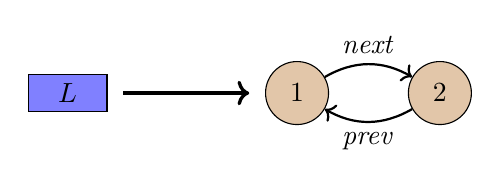
\begin{tikzpicture}
	\node[he] (lhs) {$L$};
	\node[node, ext, right=1cm and 2cm of lhs] (v1) {$1$};
	\node[node, ext, right=of v1] (v2) {$2$};
	
	\draw[->, very thick, shorten >=0.2cm, shorten <=0.2cm] (lhs) to (v1);
	\draw[sel, bend left] (v1) to node[above]{$\mathit{next}$} (v2);
	\draw[sel, bend left] (v2) to node[below]{$\mathit{prev}$} (v1);
\end{tikzpicture}
,\\
				&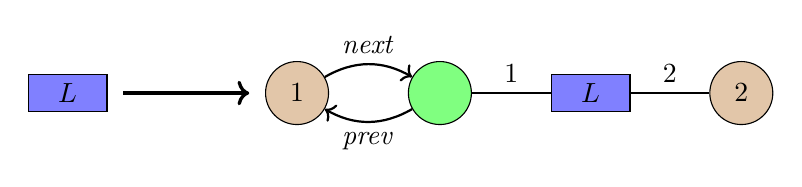
\begin{tikzpicture}
	\node[he] (lhs) {$L$};
	\node[node, ext, right=1cm and 2cm of lhs] (v1) {$1$};
	\node[node, right=of v1] (v2) {};
	\node[he, right=of v2] (e) {$L$};
	\node[node, ext, right=of e] (v3) {$2$};
	
	\draw[->,very thick, shorten >=0.2cm, shorten <=0.2cm] (lhs) to (v1);
	\draw[sel, bend left] (v1) to node[above]{$\mathit{next}$} (v2);
	\draw[sel, bend left] (v2) to node[below]{$\mathit{prev}$} (v1);
	\draw[connector] (e) to node[above]{$1$} (v2);
	\draw[connector] (e) to node[above]{$2$} (v3);
\end{tikzpicture}

			\end{aligned}
		\right\}
	\end{equation*}
	This \emph{\ac{fpHRG}} describes doublely linked list of arbitrary length.
	Firstly, it holds that
	$\type(L,1) = \{\mathit{next}\}$ and $\type(L,2) = \{\mathit{prev}\}$. But,
	consider the typed handle of $L$, where $n$, $p$ abbreviate $\mathit{next}$,
	$\mathit{prev}$ respectively:
	\begin{center}
		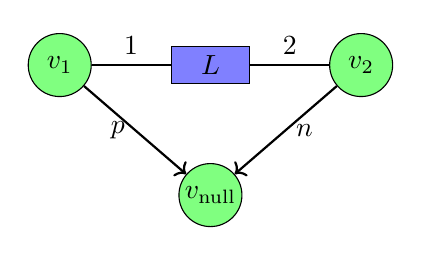
\begin{tikzpicture}
	\node[node] (v1) {$v_{1}$};
	\node[he, right=of v1] (L) {$L$};
	\node[node, right=of L] (v2) {$v_{2}$};
	\node[node, below=of L] (null) {$v_{\text{null}}$};

	\draw[connector] (L)  to node[above]{$1$} (v1)  ;
	\draw[connector] (L)  to node[above]{$2$} (v2)  ;
	\draw[sel]       (v1) to node[left] {$p$} (null);
	\draw[sel]       (v2) to node[right]{$n$} (null);

\end{tikzpicture}

	\end{center}
	In order to reveal the abstracted selectors at the tentacle $(L,2)$ only
	the first production rule can be applied. But this reduces the language to
	the singleton set of the right hand side of the first production rule.
	Repeatedly applying the second production rule does not reveal the
	abstracted selectors. Thus this grammar is not locally concretisable.
	Adding the production rule
	\begin{equation*}
		\label{eq:listrule3}
		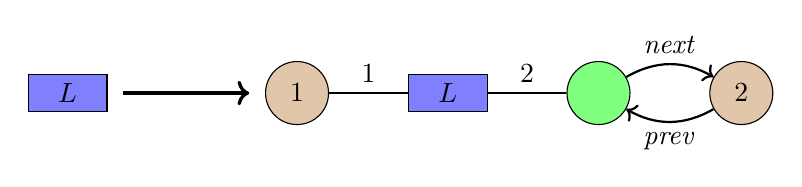
\begin{tikzpicture}
	\node[he] (lhs) {$L$};
	\node[node, ext, right=1cm and 2cm of lhs] (v1) {$1$};
	\node[he, right=of v1] (e) {$L$};
	\node[node, right=of e] (v2) {};
	\node[node, ext, right=of v2] (v3) {$2$};
	
	\draw[->,very thick, shorten >=0.2cm, shorten <=0.2cm] (lhs) to (v1);
	\draw[sel, bend left] (v2) to node[above]{$\mathit{next}$} (v3);
	\draw[sel, bend left] (v3) to node[below]{$\mathit{prev}$} (v2);
	\draw[connector] (e) to node[above]{$1$} (v1);
	\draw[connector] (e) to node[above]{$2$} (v2);
\end{tikzpicture}

	\end{equation*}
	establishes local concretisability because it is now possible to reveal
	abstracted selectors at tentacle $(L,2)$ but the generated language (doubly
	linked lists of arbitrary length) is preserved.
	
	The formal definition of local concretisability requires some additional
	defintions, such as: $(X, i)\rightarrow_{p}(Y,j)$ denotes that for a
	production rule $p\colon X\rightarrow H$ there is an edge $e\in E_{H}$ such that
	$\lab_{H}(e) = Y$ and $\ext_{H}(i) = \con_{H}(e)(j)$. This means that after
	applying the production rule $p$ the tentacle $(X, i)$ morphs (for the
	connected node) to a tentacle $(Y, j)$. Furthermore let $\overline{G^{X}}$
	denote the set of production rules in a \emph{\ac{fpHRG}} $G$ for all
	nonterminals except of $X$, i.e. $\overline{G^{X}} = G\setminus G^{X}$. Then
	local concretisability can be defined as follows:
	\begin{definition}[Local Concretisability]
		$G\in\fpHRG$ is called \emph{local concretisable} if for all nonterminals
		$X$ there are sub-grammars $G_{1},\dots,G_{\rk(X)}\subseteq G$ such
		that $\forall i\in\{1,\dots,\rk(X)\}.L_{G_{i}^{X}\cup\overline{G^{X}}}
		(X^{\bullet})=L_{G}(X^{\bullet})$ and $\forall i\in\{1,\dots,\rk(X)\}.
		\forall p\in G_{i}^{X}.(X,i)\rightarrow_{p}(a,1)$ for all selectors $a$
		in $\type(X,i)$.
	\end{definition}

	The following definition gathers now all \emph{\ac{fpHRG}} for which the
	language of the typed handle contains only valid \emph{\ac{HC}}. This
	ensures that not external nodes of the right hand sides are properly typed
	and follow the properties of \emph{\acp{HC}}.
	\begin{definition}[Data Structure Grammar]
		A \emph{\ac{HRG}} $G\in\fpHRG$ is called a \emph{\ac{DSG}}
		if it is typed and for all \emph{nonterminals} $X\in N$ the language of
		its typed handle $X^{\circ}$ only contains valid \emph{\aclp{HC}}
		($L_{G}(X^{\circ})\subseteq\HC$) and for all inner nodes of right hand
		sides in $G^{X}$ it holds that there is one outgoing edge for every
		selector in $\bigcup_{1\leq i\leq\rk(X)}\type(X,i)$.
	\end{definition}
	Note that it is assumed that only the selectors exist which are gathered
	in the different types of the tentacles of the nonterminal. If more
	selectors exist they can be simply attached to every node and point to
	$v_{\text{null}}$ to ensure that the \emph{\acp{HG}} of the language are
	still valid \emph{\acp{HC}}. Again let $\DSG$ denote the set of all
	\emph{\acp{DSG}} over $\Sigma_{N}$ and $\PI$. Additionally, it is generally
	assumend that right hand sides of production rules do not contain any edges
	labeled with variables or placeholders (thus, $\rhs(G)\subseteq
	\mathit{HG}^{\PI}_{\Sigma_{N}\setminus (\Var\cup\mathbb{T})}$). And
	therefore all inner nodes are properly typed which means that they have
	edges for all selectors that exist within the context of the nonterminal
	(i.e. the union of the types of all tentacles).
	In the following \emph{\aclp*{HAG}} are defined which are \emph{\acp{DSG}}
	that additionally provide the properties introduced above:
	\begin{definition}[Heap Abstraction Grammar]
		$G\in\DSG$ is called a \emph{\ac{HAG}} over $\Sigma_{N}$ if $G$ provides
		the following properties:
		\begin{enumerate}
			\item \emph{Productivity}
			\item \emph{Increasingness}
			\item \emph{Local Concretisability}
		\end{enumerate}
	\end{definition}
	This is no real restriction since the following theorem can be derived from
	the results of \cite{LocalGreibachNormalForm}:
	\begin{theorem}
		For every \emph{\ac{DSG}} a \emph{\ac{HAG}} can be constructed which is
		equivalent regarding the language of \emph{\acp{HG}}.
	\end{theorem}


\subsection{Concretisation}
	The basic idea of abstraction is to represent multiple heaps in one
	\emph{\ac{HG}}. Therefore \emph{\acp{HAG}} are used. Recall the
	initial programming example in Listing \ref{lst:ExampleProgram} where one
	possible execution is represented in Figure \ref{fig:BinTreeProgLang}.
	Analysing executions on binary trees of arbitrary size is realised by
	representing these as one single $B$-labeled hyperedge as follows:
	\begin{center}
		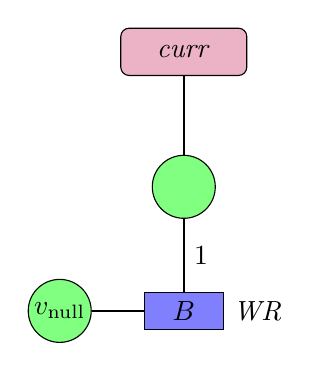
\begin{tikzpicture}
	\node[var]                 (curr) {$\mathit{curr}$};
	\node[node, below=of curr] (v)    {};
	\node[node, below left=of v] (null) {$v_{\text{null}}$};
	\node[he, label={0:{$\mathit{WR}$}}] (e) at (null-|v) {$B$};

	\draw[connector] (curr) to                  (v);
	\draw[connector] (e)    to node[right]{$1$} (v);
	\draw[connector] (e)    to                  (null);
\end{tikzpicture}

		\label{tikz:abstractedbintree}
	\end{center}
	where the \emph{\ac{fpHRG}} $G$ from page \pageref{eq:G} (which is actually
	a \emph{\ac{HAG}}) is used to derive the concrete binary trees which are
	represented by the nonterminal $B$. By applying the different production
	rules of $G$ all possible binary trees can be derived. Especially since all
	possible binary trees need to be analysed it is necessary that \emph{every}
	production rule is used to concretise the nonterminal. This leads to four
	possible representations, namely the four right hand sides of the production
	rules in $G$ (as it can be seen in Figure \ref{fig:bintreeconc}).
	\begin{figure}
		\begin{center}
			\begin{tikzpicture}
				\node (1)             {\begin{tikzpicture}
	\node[node] (v1) {$1$};
	\node[node, below left= of v1] (v2) {};
	\node[node, below right=of v1] (v3) {};
	\node[var, above=of v1] (curr) {$\mathit{curr}$};

	\draw[connector] (curr) to (v1);
	\draw[sel] (v1) to node[left] {$l_{\mathit{WR}}$} (v2);
	\draw[sel] (v1) to node[right]{$r_{\mathit{WR}}$} (v3);
\end{tikzpicture}
};
				\node[right=of 1] (d1) {};
				\node[right=of d1] (2) {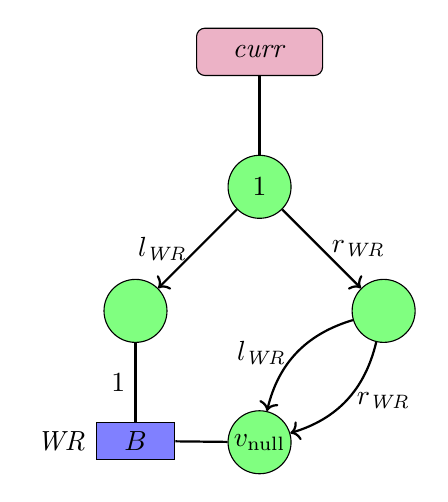
\begin{tikzpicture}
	\node[var] (curr) {$\mathit{curr}$};
	\node[node, below=of curr] (v1) {$1$};
	\node[node, below left= of v1] (v2) {};
	\node[node, below right=of v1] (v3) {};
	\node[he, below=of v2, label=180:{$\mathit{WR}$}] (e1) {$B$};
	\node[node, below=2.43 and 2 of v1] (null) {$v_{\text{null}}$};

	\draw[sel] (v1) to node[left] {$l_{\mathit{WR}}$} (v2);
	\draw[sel] (v1) to node[right]{$r_{\mathit{WR}}$} (v3);
	\draw[connector] (v2) to node[left]{$1$} (e1);
	\draw[connector] (e1) to (null);
	\draw[connector] (curr) to (v1);
	\draw[sel, bend right] (v3) to node[left]{$l_{\mathit{WR}}$} (null);
	\draw[sel, bend left] (v3) to node[right]{$r_{\mathit{WR}}$} (null);
\end{tikzpicture}
};
				\node[below=of 1] (d3) {};
				\node[below=of d3] (3) {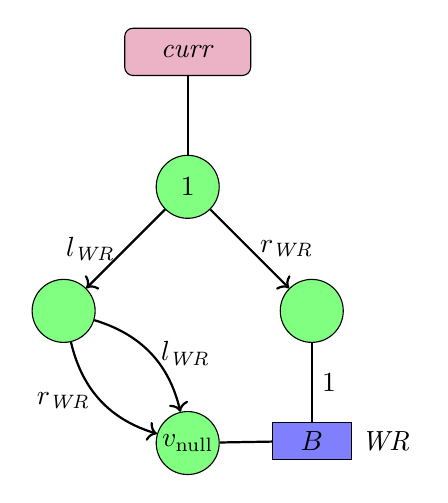
\begin{tikzpicture}
	\node[var] (curr) {$\mathit{curr}$};
	\node[node, below=of curr] (v1) {$1$};
	\node[node, below left=of v1] (v2) {};
	\node[node, below right=of v1] (v3) {};
	\node[he, below=of v3, label=0:{$\mathit{WR}$}] (e1) {$B$};
	\node[node, below=2.44 and 2 of v1] (null) {$v_{\text{null}}$};

	\draw[sel] (v1) to node[left] {$l_{\mathit{WR}}$} (v2);
	\draw[sel] (v1) to node[right]{$r_{\mathit{WR}}$} (v3);
	\draw[connector] (v3) to node[right]{$1$} (e1);
	\draw[connector] (e1) to (null);
	\draw[connector] (curr) to (v1);
	\draw[sel, bend left] (v2) to node[right]{$l_{\mathit{WR}}$} (null);
	\draw[sel, bend right] (v2) to node[left]{$r_{\mathit{WR}}$} (null);
\end{tikzpicture}
};
				\node (d2) at (d3-|2) {};
				\node (4) at (3-|2)   {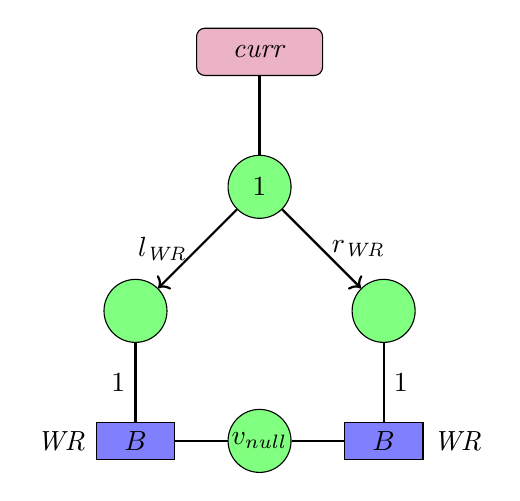
\begin{tikzpicture}
	\node[var] (curr) {$\mathit{curr}$};
	\node[node, below=of curr] (v1) {$1$};
	\node[node, below left=of v1] (v2) {};
	\node[node, below right=of v1] (v3) {};
	\node[he, below=of v3, label=0:{$\mathit{WR}$}] (e2) {$B$};
	\node[he, below=of v2, label=180:{$\mathit{WR}$}] (e1) {$B$};
	\node[node] (null) at (e2-|curr) {$v_{null}$};

	\draw[sel] (v1) to node[left] {$l_{\mathit{WR}}$} (v2);
	\draw[sel] (v1) to node[right]{$r_{\mathit{WR}}$} (v3);
	\draw[connector] (v3) to node[right]{$1$} (e2);
	\draw[connector] (v2) to node[left] {$1$} (e1);
	\draw[connector] (e1) to (null);
	\draw[connector] (e2) to (null);
	\draw[connector] (curr) to (v1);
\end{tikzpicture}
};
				\node (d4) at (4-|d1) {};

				\draw (d1) to (d4);
				\draw (d2) to (d3);
			\end{tikzpicture}
		\end{center}
		\caption{First step of concretisation for abstraction of binary trees,
			note that the permission of the nonterminal propagates to the inserted
		right hand side}
		\label{fig:bintreeconc}
	\end{figure}
	For the three \emph{\acp{HC}} that still contain nonterminals
	further concretisation steps have to be applied. But since the given
	programming language (see section \ref{sec:syntax}) allows only
	dereferences of depth one (like $x.s$) it is possible to execute all
	statements (besides fork and join) on these partially abstract
	\emph{\acp{HC}} just like they are executed on fully concrete
	\emph{\acp{HC}}. These states of partially abstract \emph{\acp{HC}} are
	called \emph{admissible} and ensure that all actually from statements
	referenceable selectors are present in the \emph{\ac{HC}}. For the formal
	definition another kind of tentacle is examined, the \emph{reduction
	tentacle}. Reduction tentacles are tentacles for which in every
	concretisation there is no outgoing edge for the identified node. This can
	be formally defined as follows:
	\begin{definition}[Reduction Tentacle]
		Let for the tentacle $(X,i)$ $v_i^{\bullet}\in V_{X^{\bullet}}$ be the 
		node such that $\con_{X^{\bullet}}(e)(i) = v_{i}^{\bullet}$ for the only
		edge $e\in E_{X^{\bullet}}$ with $\lab_{X^{\bullet}}(e) = X$ is called
		a \emph{reduction tentacle} if
		\begin{equation*}
			\forall H\in L(X^{\bullet}).\out(v_{i}^{\bullet}) = \emptyset
		\end{equation*}
	\end{definition}
	For typed nonterminals another characterisation of reduction tentacles is
	that the type of the tentacle $(X,i)$ is empty ($\type(X,i) = \emptyset$).
	As seen in \cite{LocalGreibachNormalForm} reduction tentacles can be
	determined by a syntactical analysis of the used production rules.
	Admissibility can be defined in terms of \emph{violation points} where
	violation points are tentacles that hide possibly accessible selectors.
	Formally:
	\begin{definition}[Violation Point]
		For $H\in\HC$ the tupel $(e, i)$ with $e\in E_{H}$, $\lab_{H}(e)\in N$
		and $1\leq i \leq \rk(\lab_{H}(e))$ is called a violation point, if $e$
		hides accessible selectors (i.e. there exists $e'\in E_{H}$ such that
		$\lab_{H}(e')\in\Var$ and $\con_{H}(e')(1) = \con_{H}(e)(i)$ and
		$(\lab_{H}(e),i)$ is no reduction tentacle.
	\end{definition}
	A \emph{\ac{HC}} $H$ is called \emph{admissible} if there is no violation
	point in $H$, the set of admissible \emph{\acp{HC}} is denoted by $\AHC$.
	Reconsider the abstracted representation of binary trees on page
	\pageref{tikz:abstractedbintree} which is not admissible since the tentacle
	$(B,1)$ hides the selectors $l$ and $r$ but those are actually referenceable
	by $\mathit{curr}.l$ or $\mathit{curr}.r$ respectively (when $b$ is the
	edge of the heap such that $\lab(b) = B$ then $(b,1)$ is the violation
	point). On the other hand the heap representations in Figure
	\ref{fig:bintreeconc} are admissible since the violation point is resolved
	by applying concretisation. In the following resolving violation points and
	therefore reestablishing admissibility is formalised for a \emph{\acp{HAG}}
	$G$ in the \enquote{re-admissibility} function
	\begin{equation*}
		\rea_{G}\colon\HCN\rightarrow\mathbb{P}(\AHC)
	\end{equation*}
	which maps possible abstracted \emph{\acp{HC}} to the set of admissible
	\emph{\acp{HC}} that arise by resolving violation points by applying
	production rules. But in fact not \emph{every} production rule have to be
	applied, recall therefore the \emph{\ac{fpHRG}} $G'$ of doubly linked list
	from page \pageref{eq:G'}. Imagine now a program that traverses doubly
	linked lists of arbitrary length from the last element to the first. In
	order to resolve the violation point caused by the tentacle $(L,2)$ the
	second production rule does not remove the violation point.
	But the production rule which was added to establish local
	concretisability can be used to resolve the violation point. Additionally,
	it can easily be seen that in order to establish admissibility for
	\emph{\acp{HC}} different nonterminals have to be concretised (simply
	imagine a node that is the head of a doubly linked list as well as the root
	of a binary tree and is therefore connected to a nonterminal $B$ and a
	nonterminal $L$).  Since the parts that results from concretisation of
	nonterminals are only connected via the nodes connected to the nonterminals
	and apart from that are independent it can be seen that the order in which
	\emph{\acp{HR}} are applied is insignificant to the resulting
	\emph{\ac{HG}}. This property is called \emph{confluence} and defined as
	follows:
	\begin{definition}[Confluence]
		For $H\in\HGN$ with $e_1,e_2\in E_{H}$, $e_1\neq e_2$ and $\lab_{H}(e_1),
		\lab_{H}(e_2)\in N$ it holds for two production rules
		$p_1:\lab_{H}(e_1)\rightarrow H_1$, $p_2:\lab_{H}(e_2)\rightarrow H_2$
		that
		\begin{equation*}
			H[e_1/H_1][e_2/H_2] = H[e_2/H_2][e_1/H_1]
		\end{equation*}
	\end{definition}
	As stated in \cite[p. 105]{HandbookGraphGrammars} \emph{\acp{HR}} always are
	confluent. And from this follows the following lemma (for details see
	\cite{fmsd}):
	\begin{lemma}
		\label{theo:overapprox}
		For $G\in\HAG$, $H\in\HCN$, $e\in E_{H}$ and $\lab_{H}(e)\in N$ holds
		that:
		\begin{equation*}
			L_{G}(H) = \bigcup_{\lab_{H}(e)\rightarrow K} L_{G}(H[e/K])
		\end{equation*}
	\end{lemma}
	This lemma as well as the definition of local concretisability ensures that
	applying $\rea_{G}$ still yields all possible \emph{\acp{HC}} that can be
	concretised from the \emph{\ac{HC}} $rea_{G}$ is applied to.
\subsection{Abstraction}
\label{sec:abstraction}
	After having introduced how to obtain more concrete heap
	representations from an abstracted representation in the following it is
	discussed how concrete heap representations are abstracted into more general
	representations. The idea of such an abstraction is to apply production
	rules in a backward fashion. Thus identifying the right hand side of a
	production rule, removing it and replacing it by the according nonterminal.
	Note that this approach corresponds to the way write access is handed over
	to forked processes where also subgraphs are replaced by hyperedges. For a
	comprehensible presentation of this concept recall once
	again the grammar $G$ from page \pageref{eq:G} and also consider the heap
	representation and abstraction steps in Figure \ref{fig:bintreeabs}.
	\begin{figure}
		\begin{center}
			\resizebox{\linewidth}{!}{%
				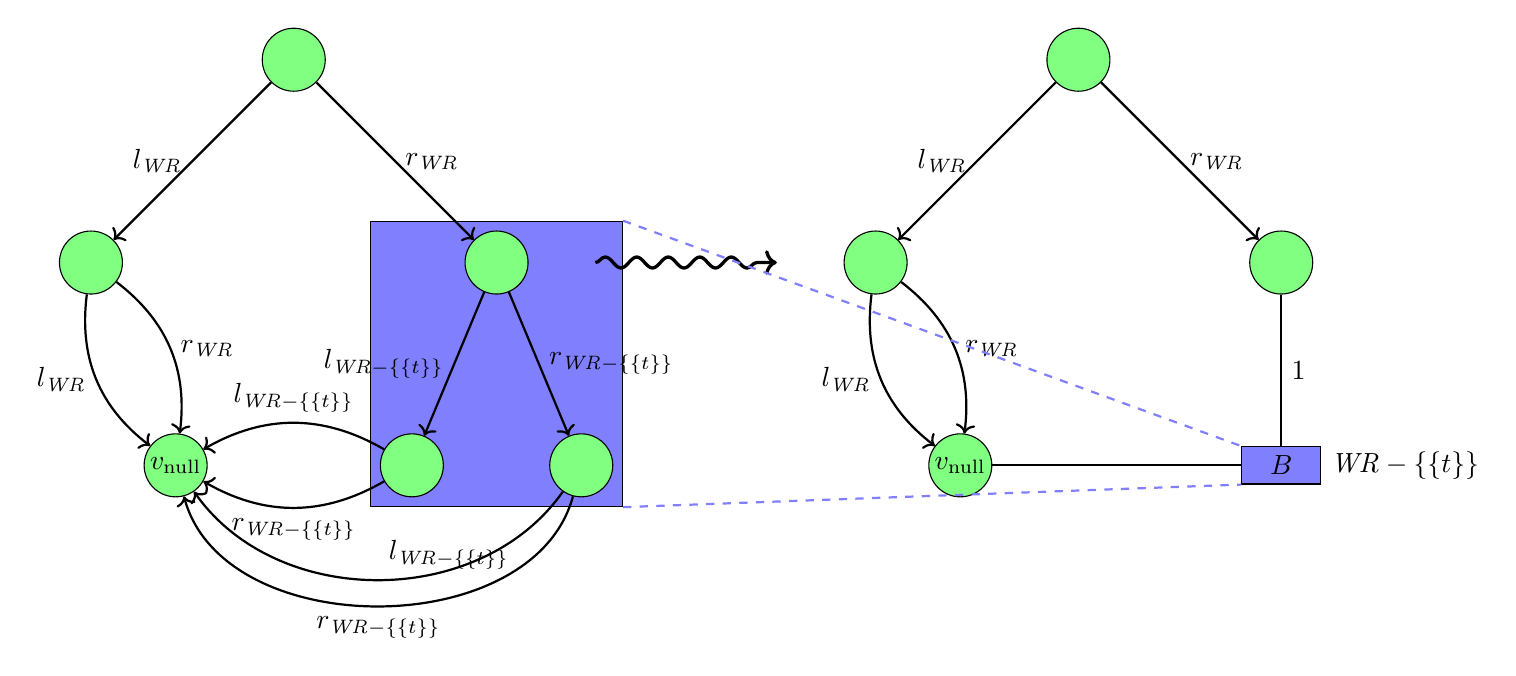
\begin{tikzpicture}[node distance=2 and 2]
	\node [node] (v1) {};
	\node [node, below left=of v1] (v2) {};
	\node [node, below right=of v1] (v3) {};
	\node [node, below left=2 and 0.5 of v3] (v4) {};
	\node [node, below right=2 and 0.5 of v3] (v5) {};
	\node [node, right =4 of v3] (v6) {};
	\node [node, above right=of v6] (v7) {};
	\node [node, below right=of v7] (v8) {};
	\node [node, below right= 2 and 0.5 of v2] (null1) {$v_{\text{null}}$};
	\node [node, below right= 2 and 0.5 of v6] (null2) {$v_{\text{null}}$};
	\node [he, label={0:$\mathit{WR}-\{\{t\}\}$}] (b) at (null2-|v8) {$B$};

	%left
	\draw [sel] (v1) to node[left]{$l_{\mathit{WR}}$} (v2);
	\draw [sel] (v1) to node[right]{$r_{\mathit{WR}}$} (v3);
	\draw [sel, bend right] (v2) to node[left]{$l_{\mathit{WR}}$} (null1);
	\draw [sel, bend left] (v2) to node[right]{$r_{\mathit{WR}}$} (null1);
	\draw [sel] (v3) to node[left]{$l_{\mathit{WR}-\{\{t\}\}}$} (v4);
	\draw [sel] (v3) to node[right]{$r_{\mathit{WR}-\{\{t\}\}}$} (v5);
	\draw [sel, bend right] (v4) to node[above]{$l_{\mathit{WR}-\{\{t\}\}}$} (null1);
	\draw [sel, bend left] (v4) to node[below]{$r_{\mathit{WR}-\{\{t\}\}}$} (null1);
	\draw [sel, bend left=55] (v5) to node[above right]{$l_{\mathit{WR}-\{\{t\}\}}$} (null1);
	\draw [sel, bend left=75] (v5) to node[below]{$r_{\mathit{WR}-\{\{t\}\}}$} (null1);

	%right
	\draw [sel] (v7) to node[left]{$l_{\mathit{WR}}$} (v6);
	\draw [sel] (v7) to node[right]{$r_{\mathit{WR}}$} (v8);
	\draw [sel, bend right] (v6) to node[left]{$l_{\mathit{WR}}$} (null2);
	\draw [sel, bend left] (v6) to node[right]{$r_{\mathit{WR}}$} (null2);
	\draw [connector] (b) to node[right]{$1$} (v8);
	\draw [connector] (b) to (null2);

	\node [right=0.6 and 0.6 of v3] (d1) {};
	\node [left=0.6 and 0.6 of v6] (d2) {};

	\draw [very thick,->, decorate,
	decoration={snake,amplitude=.7mm, segment length=4mm, post length=2mm}] (d1) to (d2);

	\begin{scope}[on background layer]
		\node [he, fit=(v3) (v4) (v5)] (layer) {};
	\end{scope}

	\draw [-, dashed, thick, color=blue!50] (layer.north east) to (b.north west); 
	\draw [-, dashed, thick, color=blue!50] (layer.south east) to (b.south west); 
\end{tikzpicture}

			}
			\caption{Heap representation of a binary tree with possible
				abstraction step}
			\label{fig:bintreeabs}
		\end{center}
	\end{figure}
	In this example the right hand side of a production rule is identified in
	the heap representation (blue mark) and replaced by the nonterminal on the
	left hand side ($B$). Note that all permissions on the right hand side of a
	production rule are the same which prevents further abstraction steps
	although besides permission the structure fits the right hand side of a
	production rule, namely the third one. But since the permissions differ
	there is no right hand side which fits this graph. For a formal approach on
	identifying the right hand side of a production rule \emph{embeddings} are
	introduced below. Embeddings are functions that identify subgraphs of
	\emph{\acp{HG}} and are formally defined as follows:
	\begin{definition}[Embedding]
		For $K,H\in\HRG$ an \emph{embedding} $\emb = (m_{V}, m_{E})$ of
		$K$ in $H$ is a pair of functions with $m_{V}:V_{K}\rightarrow V_{H}$
		and $m_{E}:E_{K}\rightarrow E_{H}$ that preserve the following
		properties:
		\begin{center}
			\begin{tabular}{|ll|}
				\hline
				$\lab_{K}(e) = \lab_{H}(m_{E}(e))$        & for all $e\in E_{K}$\\
				$\perm_{K}(e) = \perm_{H}(m_{E}(e))$      & for all $e\in E_{K}$\\
				\hline
				$m_{V}(\con_{K}(e)) = \con_{H}(m_{E}(e))$ & for all $e\in E_{K}$\\
				$\Lbag\con_{H}(e)\Rbag\cap m_{V}(V_{K}\setminus\Lbag\ext_{K}\Rbag)=
					\emptyset$                             & for all edges
					$e\in E_{H}\setminus m_E(E_{K})$\\
				\hline
				$m_{E}(e) \neq m_{E}(e')$                 & for all $e,e'\in E_{K}$
					with $e\neq e'$\\
				$m_{V}(v)\neq m_{V}(v')$                  & for all $v\in V_{K},
					v'\in V_{K} \setminus\Lbag\ext_{K}\Rbag$ with $v\neq v'$\\
				\hline
			\end{tabular}
		\end{center}
	\end{definition}
	The requirements for the functions of the embedding are as
	indicated distinguisheable in three topics:
	\begin{enumerate}
		\item Preservation, namely of labeling and permissions
		\item Structure, namely that identified edges agree on which nodes they
			connect and inner nodes are not connected to any other edge in $H$
			than those that can be also found in $K$ (since the inner nodes will
			be replaced by the nonterminal it would be unclear where those edges
			point to afterwards)
		\item Injectivity, both the embedding function of edges and nodes are
			injective with one exception: it is possible to identify multiple
			external nodes of $K$ with the same node in $H$, this causes the
			nonterminal to be connected with multiple tentacles to the same node
	\end{enumerate}
	With these definitions applying production rules backwards is defined as:
	\begin{definition}[Hyperedge introduction]
		For an \emph{\ac{HAG}} $G$, $(p_{\rho}\colon X\rightarrow M)\in G$,
		$H\in\HC$ and an embedding $(m_{V}, m_{E})$ of $K$ in $H$
		$H[M/e]\in\HGN$ is defined as follows:
		\begin{itemize}
			\item $V_{H[M/e]} = V_{H}\setminus m_{V}(V_{M}\setminus \Lbag
				\ext_{M}\Rbag)$
			\item $E_{H[M/e]} = (E_{H}\setminus m_{E}(E_{M}))\biguplus \{e\}$
			\item $\con_{H[M/e]} = \con_{H}\upharpoonright
				(E_{H}\setminus m_{E}(E_{M})) \cup \{e\mapsto m_V(\ext_{M})\}$
			\item $\lab_{H[M/e]} = \lab_{H}\upharpoonright (E_{H}
				\setminus m_{E}(E_{M})) \cup \{e\mapsto X\}$
			\item $\ext_{H[M/e]} = \ext_{H}$
			\item $\perm_{H[M/e]} = \perm_{H}\upharpoonright (E_{H}
				\setminus m_{E}(E_{M}))\cup \{e\mapsto \rho\}$
		\end{itemize}
	\end{definition}
	With these definitions an abstraction function
	\begin{equation*}
		\abs_{G}':\HGN \rightarrow\mathbb{P}(\HGN)
	\end{equation*}
	for an \emph{\ac{HAG}} $G$ is defined which maps an \emph{\ac{HG}}
	$H\in\HGN$ to the set of those \emph{\acp{HG}} that result by introducing
	successively hyperedges until there is no further embedding for any right
	hand side of any production rule in $G$. Note firstly that this way of
	abstracting terminates because $G$ is increasing and thus every abstraction
	step results in a smaller \emph{\ac{HG}} and secondly that abstraction
	might possibly lead to a set of \emph{\acp{HG}} instead of a single one as
	the following example illustrates. Consider therefore the \emph{\ac{fpHRG}}
	$G'$ from page \pageref{eq:G'} and the following example of abstraction
	steps where every arrow indicate the introduction of an hyperedge.
	\begin{center}
		\resizebox{\linewidth}{!}{%
			\begin{tikzpicture}
				\node (1) {\begin{tikzpicture}
	\node[node]              (v1) {};
	\node[node, right=of v1] (v2) {};
	\node[node, right=of v2] (v3) {};

	\draw[sel, bend left] (v1) to node[above]{$n_{\mathit{WR}}$} (v2);
	\draw[sel, bend left] (v2) to node[below]{$p_{\mathit{WR}}$} (v1);
	\draw[sel, bend left] (v2) to node[above]{$n_{\mathit{WR}}$} (v3);
	\draw[sel, bend left] (v3) to node[below]{$p_{\mathit{WR}}$} (v2);
\end{tikzpicture}

};
				\node[below left =of 1] (2) {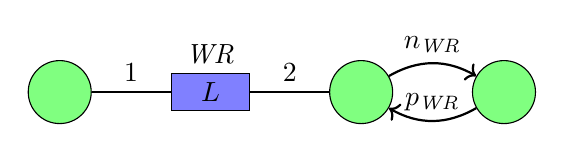
\begin{tikzpicture}
	\node[node] (v1) {};
	\node[he, right=of v1, label=90:{$\mathit{WR}$}] (L) {$L$};
	\node[node, right=of L] (v2) {};
	\node[node, right=of v2] (v3) {};

	\draw[connector] (L) to node[above]{$1$} (v1);
	\draw[connector] (L) to node[above]{$2$} (v2);
	\draw[sel, bend left] (v2) to node[above]{$n_{\mathit{WR}}$} (v3);
	\draw[sel, bend left] (v3) to node[above]{$p_{\mathit{WR}}$} (v2);
\end{tikzpicture}
};
				\node[below right=of 1] (3) {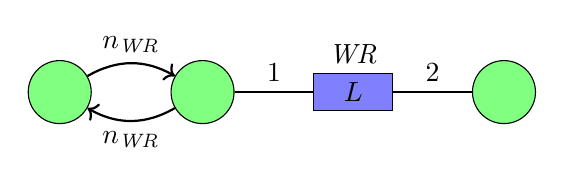
\begin{tikzpicture}
	\node[node]              (v1) {};
	\node[node, right=of v1] (v2) {};
	\node[he, right=of v2, label=90:{$\mathit{WR}$}] (e1) {$L$};
	\node[node, right=of e1] (v3) {};

	\draw[sel, bend left] (v1) to node[above]{$n_{\mathit{WR}}$} (v2);
	\draw[sel, bend left] (v2) to node[below]{$n_{\mathit{WR}}$} (v1);
	\draw[connector] (e1) to node[above]{$1$} (v2);
	\draw[connector] (e1) to node[above]{$2$} (v3);
\end{tikzpicture}
};
				\node[below =of 2]      (4) {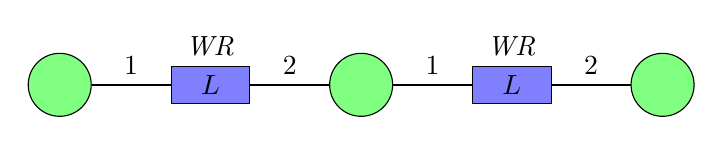
\begin{tikzpicture}
	\node[node]              (v1) {};
	\node[he, right=of v1, label=90:{$\mathit{WR}$}] (e1) {$L$};
	\node[node, right=of e1] (v2) {};
	\node[he, right=of v2, label=90:{$\mathit{WR}$}] (e2) {$L$};
	\node[node, right=of e2] (v3) {};

	\draw[connector] (e1) to node[above]{$1$} (v1);
	\draw[connector] (e1) to node[above]{$2$} (v2);
	\draw[connector] (e2) to node[above]{$1$} (v2);
	\draw[connector] (e2) to node[above]{$2$} (v3);
\end{tikzpicture}
};
				\node[below =of 3]      (5) {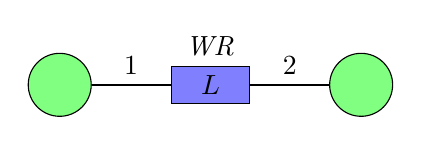
\begin{tikzpicture}
	\node[node]                                      (v1) {};
	\node[he, right=of v1, label=90:{$\mathit{WR}$}] (e)  {$L$};
	\node[node, right=of e]                          (v2) {};
	\draw[connector] (e) to node[above]{$1$} (v1);
	\draw[connector] (e) to node[above]{$2$} (v2);
\end{tikzpicture}
};
				\draw[->, thick] (1) to (2);
				\draw[->, thick] (1) to (3);
				\draw[->, thick] (2) to (4);
				\draw[->, thick, dotted] (2) to (5);
				\draw[->, thick] (3) to (4);
				\draw[->, thick] (3) to (5);
			\end{tikzpicture}
		}
	\end{center}
	Note that the dotted arrow is only valid if the third production rule (on
	page \pageref{eq:listrule3}) which established local concretisability is
	added to $G'$. Nevertheless there are two \emph{\acp{HG}} that can not be
	anymore abstracted which are obtained by introducing hyperedges repeatedly.
	As stated for \emph{\ac{HR}} it holds that two (and therefore by an
	inductive argument arbitrary many) production rules are
	applied and there is exactly one resulting \emph{\ac{HG}}, but for backward
	application there are possible multiple resulting \emph{\acp{HG}} and it
	depends on which abstraction is carried out first. Consider now adding
	additionally the production rule
	\begin{equation*}
		\label{eq:listrule4}
		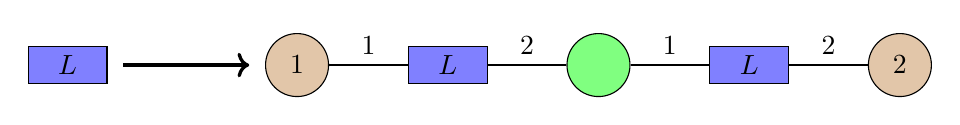
\begin{tikzpicture}
	\node[he] (lhs) {$L$};
	\node[node, ext, right=1cm and 2cm of lhs] (v1) {$1$};
	\node[he, right=of v1] (L1) {$L$};
	\node[node, right=of L1] (v2) {};
	\node[he, right=of v2] (L2) {$L$};
	\node[node, ext, right=of L2] (v3) {$2$};
	
	\draw[->, very thick, shorten >=0.2cm, shorten <=0.2cm] (lhs) to (v1);
	\draw[connector] (L1) to node[above]{$1$} (v1);
	\draw[connector] (L1) to node[above]{$2$} (v2);
	\draw[connector] (L2) to node[above]{$1$} (v2);
	\draw[connector] (L2) to node[above]{$2$} (v3);
\end{tikzpicture}

	\end{equation*}
	to $G'$. This causes the above considered abstraction to result in a
	singleton set because the left hand leaf of this \enquote{abstraction tree}
	can be further abstracted to the right hand leaf. The property that
	abstraction results in a single possible \emph{\ac{HG}} is called
	\emph{backward confluence} and a \emph{\ac{HAG}} is called backward
	confluent if every abstraction for an arbitrary \emph{\ac{HG}} results in a
	single \emph{\ac{HG}}. For a backward confluent \emph{\acp{HAG}} $G$ the
	abstraction function $\abs_{G}\colon \HGN\rightarrow\HGN$ is defined as the
	mapping from every \emph{\ac{HG}} $H$ to the single element in
	$\abs_{G}'(H)$. It is unclear if it is possible to establish backward
	confluence for \emph{\acp{HAG}}, but it is decideable if an \emph{\ac{HAG}}
	is backward confluent (for details see \cite{InductivePredicates}).

	\subsection{Abstract Semantics}
	\label{sec:abstractsemantics}
	As already mentioned above and also explored in \cite{fmsd} it is possible
	to model the semantics of statements (except fork and join) on partially
	abstracted but admissible \emph{\acp{HC}} because the admissibility ensures
	that all referenceable objects and selectors are actually currently
	available in the heap representation. But it is possible that the execution
	of such a statement invalidates the admissibility because other selectors
	can become
	referenceable because a variable might get assigned a new value. This
	inadmissibility has to be resolved in order to continue the analysis of
	further statements. In order to resolve inadmissibilities the heap
	representation is at first completely abstracted and subsequently as far as
	necessary concretised to reestablish admissibility. The first abstraction
	step is used in order to minimise the heap representation because $\rea_{G}$
	stops as soon as admissibility is established.
	With these intuitions the abstract semantics (denoted by $\btr$) of pointer
	operations (which are all statements except of fork, join and assignment of
	process identifiers) can be given as follows:
	\begin{prooftree}
		\AxiomC{$(S, H)\rhd(S',I)$}
		\AxiomC{$H'\in\rea_{G}(\abs_{G}(I))$}
		\BinaryInfC{$(S,H)\btr(S',H')$}
	\end{prooftree}
	For the semantics of the assignment of process identifiers the concrete
	semantics also transfer to partially abstracted \emph{\acp{HC}} since the
	definitions given for the modifications of permissions in Section
	\ref{sec:graphtrans} are applicable for nonterminals as well, thus no
	changes are required.

	For join and fork on the other hand some modifications in semantics have to
	be introduced. At first the postponed definitions of \emph{reachability} and
	\emph{border} nodes are addressed and afterwards the semantics of fork and
	join are applied on partially abstracted \emph{\acp{HC}}.

	The set of selectors that are reachable from an initial node are those
	selectors that can be reached via moving along other selectors. For example
	consider the \emph{\ac{HC}} described in Figure \ref{fig:reachability}.
	\begin{figure}[h]
		\begin{center}
			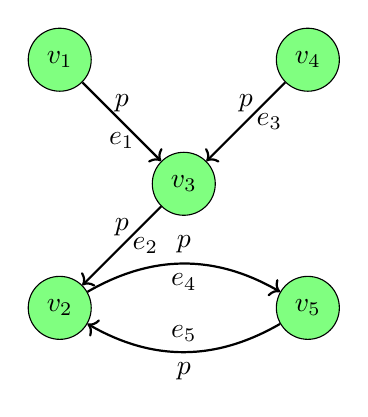
\begin{tikzpicture}
	\node[node]                (v3) {$v_{3}$};
	\node[node, above left =of v3] (v1) {$v_{1}$};
	\node[node, below left =of v3] (v2) {$v_{2}$};
	\node[node, above right=of v3] (v4) {$v_{4}$};
	\node[node, below right=of v3] (v5) {$v_{5}$};

	\draw[sel]            (v1) to node[above, label=-90:{$e_{1}$}]{$p$} (v3);
	\draw[sel]            (v3) to node[above, label={[label distance=-0.3cm]-45:
		{$e_{2}$}}]{$p$} (v2);
	\draw[sel]            (v4) to node[above, label={[label distance=-0.3cm]-45:
		{$e_{3}$}}]{$p$} (v3);
	\draw[sel, bend left] (v2) to node[above, label=-90:{$e_{4}$}]{$p$} (v5);
	\draw[sel, bend left] (v5) to node[below, label=90:{$e_{5}$}]{$p$} (v2);
\end{tikzpicture}

		\end{center}
		\caption{simple \emph{\ac{HC}} to illustrate reachability}
		\label{fig:reachability}
	\end{figure}
	The set of reachable edges from $v_{1}$ is $\{e_{1}, e_{2}, e_{4}, e_{5}\}$
	since from $v_{1}$ $e_{1}$ is directly reachable and after moving along
	$e_{1}$ the edge $e_{2}$ is reachable and so forth. On the other hand
	$e_{3}$ is not reachable from $v_{1}$ since the selector points in the
	\enquote{wrong} direction. In order to formalise these movements along the
	edges in $H\in\HGN$ the notion of a path $\pi$ is introduced as
	\begin{equation*}
		\pi \in (\mathbb{N}\times E_{H}\times \mathbb{N})^{\ast}
	\end{equation*}
	where it holds for $\pi(k) = (i,e,j)$ and $\pi(k+1) = (i',e',j')$ that
	$\con_{H}(e)(j) = \con_{H}(e')(i')$ for all $1\leq k \leq (|\pi| - 1)$. This
	describes undirected paths, i.e.
	\begin{equation*}
		(1, e_{1}, 2)(2, e_{3}, 1)
	\end{equation*}
	is a valid path although $e_{3}$ is actually not reachable from $v_{1}$.
	Thus, not all paths agree with the intuition of reachability. The intuition
	of reachability is easy for selectors which are interpreted as directed
	edges. For nonterminals reachability is understood as the possibility to
	concretise this nonterminal in a way such that there is a reachable path
	along selectors between the connected nodes. Formally defined is
	reachability by the use of the term bridge as follows:
	\begin{definition}[Reachability]
		A bridge $(i, X, j) \in \br(N\cup\Sel)$ is called \emph{reachable}
		for $G\in\HAG$ if $i = 1, j = 2, X\in\Sel$ or if $X\in N$ and there is
		$H\in L_G(X^{\bullet})$ such that there is a reachable path $\pi$ from
		$v_i^{\bullet}$ to $v_j^{\bullet}$.
	\end{definition}
	Note that it is assumed that the set $\Sel$ is ranked by the function that
	maps all selectors to $2$ to ensure that $\br(N\cup \Sel)$ is defined. A
	path $\pi$ is called reachable if every used bridge is reachable. Let
	$\Path(u,v)$ denote all paths that start in $u$ and end in $v$, formally:
	\begin{equation*}
		\Path(u,v) = \left\{\pi\mid
			\begin{aligned}
					&\pi\text{ is a path}\\
					&\land(i,e,j) =\pi(1)\land\con_{H}(e)(i)=u\\
					&\land(i',e',j') =\pi(|\pi|)\land\con_{H}(e')(j') = v
			\end{aligned}
		\right\}
	\end{equation*}

	Furthermore it is possible to compute all reachable bridges over
	nonterminals in a \emph{\ac{HAG}} over syntactical analysis of the
	\emph{\ac{HAG}} as the following lemma states:
	\begin{lemma}
		For $G\in\HAG$ the set $\RB(G)$ denotes all \emph{reachable}
		\emph{bridges} in $G$. $\RB(G)$ can be computed by syntactical analysis
		of $G$.
	\end{lemma}
	\begin{proof}
		Let
		\begin{equation*}
			\RB_{0} =  \{(1,s,2)\mid s\in\Sel\}
		\end{equation*}	
		denote the set of all bridges over selectors in the \enquote{right}
		direction.
		Let furthermore $\NT(\pi)$ denote all used bridges in the path $\pi$ in
		an \emph{\ac{HG}} $H$
		\begin{equation*}
			\NT(\pi)=
				\left\{
					(i,\lab_H(e), j)\mid (i,e, j)\in\Lbag\pi\Rbag
				\right\}
		\end{equation*}
		then
		\begin{equation*}
			\RB_{n+1} = \{(i,X,j)\mid\exists H\in\rhs(G^{X}).
			\exists \pi\in\Path(\ext_{H}(i),\ext_{H}(j)).\NT(\pi)
			\subseteq\mathit{RB}_{n}\}
		\end{equation*}
		denote the set of all reachable bridges that make use of
		previously computed reachable bridges which ensure reachable paths. For
		example, $\RB_{1}$ is the set of bridges over selectors and those
		nonterminals for which a right hand side of a production rule exists
		where a path along selectors connects $\ext_{H}(i)$ and $\ext_{H}(j)$.
		It is easy to see that this iteration is monotone and since the set of
		all bridges for a finite set of nonterminals $N$ and selectors $\Sel$ is
		finite as well it terminates after finitly many steps. By induction over
		$n$, the depth of applied concretisation steps for nonterminals until a
		reachable path is found it follows that the fixpoint of this iteration
		is indeed $\RB(G)$.
	\end{proof}
	Combining this result with a breadth-first search that computes stepwise all
	possible paths of finite length and with the set $\RB(G)$ it can be tested
	if these paths are reachable. It follows that for a finite graph all
	reachable paths can be computed. Let $\CPath_{H}(v)$ denote all reachable
	paths in $H$ starting in the node $v$:
	\begin{corollary}
		For $H\in\HGN$, $G\in\HAG$ and $v\in V_{H}$ the set $\CPath_{H}(v)$ can
		be computed by syntactical analysis of $G$ and a structural analysis of
		$H$.
	\end{corollary}
	Another point has to be taken into account before the set of reachable edges
	can be formally defined. It is illustrated by the following production rule:
	\begin{equation*}
		\label{eq:reachex}
		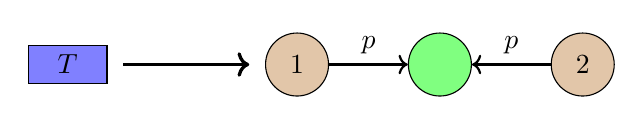
\begin{tikzpicture}
	\node[he] (lhs) {$T$};
	\node[node, ext, right=1cm and 2cm of lhs] (v1) {$1$};
	\node[node, right=of v1] (v2) {};
	\node[node, ext, right=of v2] (v3) {$2$};

	\draw[->, very thick, shorten >=0.2cm, shorten <=0.2cm] (lhs) to (v1);
	\draw[sel] (v1) to node[above]{$p$} (v2);
	\draw[sel] (v3) to node[above]{$p$} (v2);
\end{tikzpicture}

	\end{equation*}
	It is evident that the bridges $(1,T,2), (2,T,1)$ are both not reachable.
	But also both tentacles $(T,1), (T,2)$ are not reduction tentacles since
	both actually abstract selectors. If any reachable path from a starting node
	$u$ to a node $v$ exists such that $v$ is connected to a $T$-labeled edge
	$e$, then $e$ has to be included in the set of reachable edges, since it
	abstracts edges which can actually be reached.
	With this in mind the set of reachable edges from a node $v$ in a
	\emph{\ac{HG}} $H$ denoted by $\reach_{\text{abs}}^{H}(v)$ can be formally
	defined in two steps. First all edges of reachable paths are gathered in
	\begin{equation*}
		P = \{e \mid (i, e, j)\in\Lbag\pi\Rbag,\pi\in\CPath_{H}(v)\}
	\end{equation*}
	and secondly all nonterminals where parts of the concretisating graphs can
	be reached in
	\begin{equation*}
		D = 
		\left\{e\mid
			\begin{aligned}
				&\lab_{H}(e)\in N, 1\leq i\leq \rk(\lab_{H}(e)).
				\exists e'\in P.\con_{H}(e)(i)\in\Lbag\con_{H}(e')\Rbag\\
				&\land (\lab_{H}(e),i)\text{ is no reduction tentacle}
			\end{aligned}
		\right\}
	\end{equation*}
	Then the set of reachable edges is defined as:
	\begin{equation*}
		\reach_{\text{abs}}^{H}(v) = P\cup D
	\end{equation*}
	and let
	\begin{equation*}
		\reach_{\text{abs}}^{H}(v_1,\dots,v_n) = \bigcup_{1\leq i\leq n}
		\reach_{\text{abs}}^{H}(v_i)
	\end{equation*}
	denote the reachable nodes from multiple initial nodes.
	This concludes computing the reachable edges in a partially abstract
	\emph{\ac{HG}}. As mentioned before the computation of reachable edges for
	fully concrete \emph{\acp{HG}} relies on the reachability in the abstracted
	case and is intuitively achieved by abstracting the concrete \emph{\ac{HG}},
	computating the set of reachable edges, concretising with the same sequence
	of production rules that is used for the abstraction to rebuild the initial
	\emph{\ac{HG}}. The set of reachable edges in the concrete
	\emph{\ac{HG}} are all edges that arise from reachable edge in the
	abstraction. Therefore \emph{production sequences}
	are introduced as sequence of tupel of production rules and edges. A
	production sequence denotes the way a heap is transformed via production
	rules. This means it is possible to revert abstraction steps by saving
	tupels of the production rules and the introduced hyperedges that arise from
	backward application of that production rule and applying this sequence in
	reversed order to the abstracted \emph{\ac{HG}} yields again the original
	concrete \emph{\ac{HG}}. Let $\pi$ be a finite production
	sequence then $\pi^{-1}$ denotes the reversed production sequence.
	Furthermore let $\pi\upharpoonright E$ denote the production sequence that
	contains all production rules in $\pi$ that are applied to edges in $E$ or
	edges that are concretised from $E$ (in possibly multiple applications of
	production rules). Let furthermore $H\xRightarrow{\pi} Q$ denote
	the application of a sequence of production rules $\pi$. Especially it holds
	for the production sequence $\pi$ which is used to obtain $\abs_{G}(H)$ that
	$\abs_{G}(H)\xRightarrow{\pi^{-1}} H$.  Additionally, let $H$ be a partially
	abstracted \emph{\ac{HG}} then let $E_{\pi}$ for an production sequence
	$\pi$ denote the set of all edges that arise from concretisation steps
	applied to edges of $E$ and edges that are originally obtained from edges in
	$E$.
	\begin{equation*}
		E_{\pi} = \{e\mid (H\upharpoonright E)\xRightarrow
			{\pi\upharpoonright E}H', e\in E_{H'}\}
	\end{equation*}
	With these notions reachability for concrete hypergraphs can be defined
	in context of a \emph{\ac{HAG}} $G$ as follows:
	\begin{equation*}
		\reach_H(v_{1},\dots,v_{n}) = (\reach_{\text{abs}}^{\abs_{G}(H)}(v_{1},
		\dots,v_{n}))_{\pi^{-1}}
	\end{equation*}
	where the abstraction preserves $v_{1}, \dots, v_{n}$ and $\pi$ denotes the
	corresponding production sequence of the abstraction.

	For the contracts of the forked programs there is one difference to the
	concrete semantics which is that a partially abstract precondition
	concretises to various possible \emph{\acp{HC}} (similar to the contracts
	presented in \cite{ProcedureSummaries}). Just like concretisation
	of nonterminals demands that all production rules that establish
	admissibility are analysed (since the information from which of these
	concrete \emph{\acp{HC}} it is abstracted from is lost) there are also
	multiple postconditions that might apply after the execution of a program
	depending on the actual structures the partially abstract precondition
	concretises to. Formally, this leads to a set of contracts for a program $m$
	where one precondition leads to multiple postconditions:
	\begin{equation*}
		\Cont_{\text{abs}}(m)\subseteq
		\mathbb{P}((\HGN\times\mathbb{P}(E)\times
		\mathbb{P}(\mathit{HG}^{\PI'}_{\Sigma_{N}'})))
	\end{equation*}
	where for every $C = (P_{C}, E_{C}, \mathbb{Q}_{C})\in\Cont_{\text{abs}}(m)$
	holds that $E_{C}\subseteq E_{\mathit{WR}}^{P_{C}}$.
	Furthermore there is for every program $m$ and
	precondition $P$ maximal one contract $C\in\Cont_{\text{abs}}(m)$. Because
	if there are two contracts $C,C'\in\Cont_{\text{abs}}(m)$ with
	$P_C\afiso P\afiso P_{C'}$ then those contracts can be united to a contract
	$C'' = (P, E_{C}\cup E_{C'}, \mathbb{Q}')$ such that $\mathbb{Q}'$ contains
	all possible results from executions of $m$ starting from the initial
	heap state (which is obtained from the precondition and the set of
	alternable edges the same way it is described in Section \ref{sec:join}
	with straightforward ajustments for nonterminals).

	As already introduced the intuition for border nodes is that these nodes
	are part of the subgraph for which the access tickets are transferred to the
	newly forked process but are also still part and accessible (with limitation
	to some selectors) to the forking process.
	For the formal definition let $H$ be the current heap representation, 
	$C = (P_C, E_C, \mathbb{Q}_C)$ be a contract for the forked process, $R$ be
	the reachable subgraph from the actual parameter of the fork statement and
	it holds that $R\afiso P_C$. Then the set of border nodes can be defined as
	follows:
	\begin{equation*}
		\border_{\text{abs}}^{H}(C) = \left(\bigcup_{e\in E_{C}}\Lbag\con_{H}(e)
		\Rbag\right)\bigcap\left(\bigcup_{e\in E_{H}\setminus E_{C}}
		\Lbag\con_{H}(e)\Rbag\right)
	\end{equation*}
	which leads to the following transformation of the heap representation of
	the forking process:
	\begin{equation*}
		H' = H[\downarrow t][\setminus E_{C}][+_\mathit{WR}N_{\{t\}}
		\rightrightarrows \mathit{enum}_{b_{C}(H)}]
		[(E_{P_{C}}\setminus E_{C}) - \{t\}]
	\end{equation*}
	where $t$ denotes the process identifier that identifies the newly forked
	process initially.
	With these definitions the abstract semantics for the fork statement can be
	given as follows where
	$R=(H\upharpoonright \reach_{\text{abs}}(\llbracket x_{1}\rrbracket_{H},
		\dots,\llbracket x_{n}\rrbracket_{H}))$
	\begin{prooftree}
		\AxiomC{$(P_{C},E_{C},\mathbb{Q}_{C})\in\Cont_{\text{abs}}(m)$}
		\AxiomC{$P_{C} \afiso R$}
		\AxiomC{$H'' \in \rea_{G}(\abs_{G}(H'))$}
		\TrinaryInfC{$(t=\text{fork}(m(x_{1},\dots,x_n)),H)\btr(\varepsilon,H'')
		$}
	\end{prooftree}

	Lastly, the join statement is dealt with almost the same as in the
	concrete semantics. Recall therefore the two transformations steps for one
	precondition $Q$ from page \pageref{eq:joinH}:
	\begin{equation*}
		Q'_{1}=Q_{C}[\downarrow\mathit{enum}_{\mathit{Var}'_{\text{thread}}}(1)]
		\dots[\downarrow\mathit{Var}'_{\text{thread}}
		(|\mathit{Var}'_{\text{thread}}|)]
	\end{equation*}
	and
	\begin{equation*}
		Q'_{2} = Q'_{1}[\setminus (E^{Q'_{1}}_{\mathit{RD}}\cup
			E^{Q'_{1}}_{\mathit{RD^{\ast}}})]
	\end{equation*}
	then there are again two transition rules for the join statement where
	one deals with fully returned read tickets and the other one with lost
	read tickets. Especially \emph{every} postcondition $Q\in\mathbb{Q_C}$
	is examined (since every postcondition describes a valid execution of
	the program from the initial heap state).
	\begin{prooftree}
		\AxiomC{$Q\in\mathbb{Q}_{C}$}
		\AxiomC{$E^{Q'_{1}}_{\mathit{RD^{\ast}}}\neq\emptyset$}
		\AxiomC{$H[\downarrow T_{t}]\xRightarrow{N_{T_{t}}\rightarrow Q'_{2}}H'$}
		\AxiomC{$H''\in\rea_{G}(\abs_{G}(H'))$}
		\QuaternaryInfC{$(\text{join}(t), H)\btr(\varepsilon,H'')$}
	\end{prooftree}
	\begin{prooftree}
		\AxiomC{$Q\in\mathbb{Q}_{C}$}
		\AxiomC{$E^{Q'_{1}}_{\mathit{RD^{\ast}}}=\emptyset$}
		\AxiomC{$H[\leftarrow T_{t}]\xRightarrow{N_{T_{t}}\rightarrow Q'_{2}}H'$}
		\AxiomC{$H''\in\rea_{G}(\abs_{G}(H'))$}
		\QuaternaryInfC{$(\text{join}(t), H)\btr(\varepsilon,H'')$}
	\end{prooftree}
	where $C = (P_{C}, E_{C}, \mathbb{Q}_{C})$ is the contract which the process
	is forked by before (which can be obtained by attaching it to the
	placeholder when the fork statement is executed). Additionally it can be
	explained in the context of abstraction why it is avoided for the concrete
	semantics as well as for the abstract semantics to match the shared edges
	from the postcondition to the ones in the heap representation of the joining
	process. Because of the applied abstraction it is possible that nonterminals
	that are identified at the join statement get concretised and abstracted
	differently through the execution of both processes. To avoid accounting
	from which nonterminals different edges arose (especially since it had to be
	done for every forked process individually) it is just dealt with by
	handing over one read ticket for all shared edges and returning the minimum
	of this read ticket (nothing if any edge cannot return its ticket completely
	or everything if every edge can guarantee to return the whole ticket). Also
	this fits the approach to deal with abstraction and permissions as
	orthogonal concepts (like it is approached by introducing fully permissive
	grammars on page \pageref{def:fpg}).
	Note that again one abstraction and one
	concretisation step is applied to the resulting heap representation. This is
	done because after the transformation of permissions as well as inserting
	the \enquote{$\mathit{WR}$ part} into the heap representation it is possible
	that the right hand side of production rule can be found in the resulting
	heap representation which were not present before. Thus, to obtain the
	most general heap representation the abstraction step is executed and
	following to obtain the minimal admissible \emph{\acp{HC}} one
	concretisation step is applied.

	\subsection{Correctness}
	The main result justifying the taken approach on the presented abstraction
	is to show that $\btr$ is an over-approximation of the transition relation
	$\rhd$. Therefore it is assumed that abstraction and concretisation relies
	on a backward confluent \emph{\ac{HAG}} $G$ and abstract and concrete
	contracts are connected in the following way: For every
	$C = (P_{C}, E_{C}, Q_{C})\in\Cont(m)$ exists
	$C' = (P_{C'}, E_{C'}, \mathbb{Q}_{C'})\in\Cont_{\text{abs}}(m)$ such that
	\begin{enumerate}[label=(\roman*)]
		\item $P_{C}\in L_{G}(P_{C'})$, which implies there is a production
			sequence $\pi$ such that $P_{C'}\xRightarrow{\pi}P_{C}$
		\item  $P_{C'}\upharpoonright E_{C'}
			\xRightarrow{\pi\upharpoonright E_{C'}}P_{C}\upharpoonright E_{C}$
		\item there is $Q'\in\mathbb{Q}_{C'}$ with $Q_{C}\in L_{G}(Q')$
	\end{enumerate}
	This intuitively means that
	\begin{enumerate*}[label=(\roman*)]
		\item preconditions of concrete contracts arise from concretisation of 
			preconditions of abstract contracts, where
		\item every edge in the alternable set of the concrete contract arise
			from concretisation of edges in the alternable set of the abstract
			contract and
		\item the postcondition of the concrete contract can be found by
			concretising one of the postconditions of the abstract contract.
	\end{enumerate*}
	Note further that the order of $\pi$ does not matter due to the confluence
	property of \emph{\ac{HR}}, but a previous \emph{\ac{HR}} can expose the
	hyperedges which later production rules are applied to. This might cause
	dependencies between the production rules. A subsequence $\chi$ of
	$\pi$ denoted as $\chi\prec\pi$ is a sequence of production rules such that
	these production rules appear also in $\pi$.

	These assumptions are essential requirements for the presented analysis and
	abstraction approach of this paper. Because the actual analysis is actually
	designed for abstracted representation, it is expected that the set of
	abstracted contracts is computed first and the concrete contracts are simply
	generated by concretisation of abstracted contracts. This justifies that
	even for the concrete semantics a corresponding abstracted contract exists
	for every concrete contract. This is necessary because the border nodes for
	the concrete semantics are computed by abstracting and computing the border
	nodes for the abstracted case and concretise by the sequence of production
	rules used for the abstraction. This is necessary to ensure that the
	abstract semantics overapproximate the concrete semantics. This approach
	agrees with the intuition of the border
	nodes in the concrete semantics because the computation of border nodes in
	the abstracted \emph{\ac{HC}} is a superset of the actual border nodes.
	Recall therefore the intutition of border nodes for the
	concrete semantics as all nodes that are connected to an edge for which
	$\mathit{WR}$ permission is transferred and an edge that is still present 
	within the heap representation of the forking process. Let $H$ be this heap
	representation and $C = (P_{C}, E_{C}, Q_{C})$ the contract by which the
	fork statement is executed then the intuition translates to the following
	set:
	\begin{equation*}
		\mathit{IB}_{H}(C) = \{v\mid \exists e\in E_{C}.\exists e'\in E_{H}
			\setminus E_{C}.v\in\Lbag\con_{H}(e)\Rbag
			\cap\Lbag\con_{H}(e')\Rbag\}
	\end{equation*}
	Then the following lemma states that this computation
	ensures that the border nodes are a superset of the nodes that are
	intuitively understood as border nodes:
	\begin{lemma}[Border Lemma]
		For $C\in\Cont(m)$ and $C'\in\Cont_{\text{abs}}(m)$ such that for $C$ and
		$C'$ $(i),(ii),(iii)$ holds that
		$\mathit{IB}_{H}(C)\subseteq\border_{H}(C')$
	\end{lemma}
	Firstly one additional property for
	\emph{\ac{HR}}, namely \emph{context-freeness}, is presented in
	the following because it motivates some of the used results for the
	presented proofs. But in order to avoid some formal machinery
	context-freeness is only presented informally, for formal details as well as
	the proof that \emph{\ac{HR}} actually is context-free see
	\cite[pp. 111-115]{HandbookGraphGrammars}: The deriveration of nonterminals
	is context-free in the sense that it is independent from the rest of the
	\emph{\ac{HG}}. This means, first applying production rules to nonterminals
	and glueing the resulting hypergraphs together yields the same result as
	glueing the hypergraphs together and applying the same production rules
	afterwards. In the following the proof for the \emph{Border Lemma} is
	presented which actually makes use of context-freeness property:
	\begin{proof}[Border Lemma]
		Let $v\in\mathit{IB}_{H}(C)$ be arbitrarily chosen. It follows that
		$v\in\border_{H}(C)$ by the following argument:
		Since $v\in\mathit{IB}_{H}(C)$ it follows that there is $e\in E_{C}$ and
		$e'\in E_{H}\setminus E_{C}$ such that
		$v\in\Lbag\con_{H}(e)\Rbag\cap\Lbag\con_{H}(e')\Rbag$. Let furthermore
		$C'$ denote the abstract contract to $C$ for which $(i), (ii), (iii)$
		holds. By the context-freeness property of \emph{\ac{HR}} and because
		$(ii)$ holds follows that
		there are $e_{\text{abs}}\in E_{C'}$ and $e'_{\text{abs}}\in
		E_{\abs_{G}(H)}\setminus E_{C'}$ such that $e$ arises from concretisation
		of $e_{\text{abs}}$ and $e'$ from concretisation of $e'_{\text{abs}}$.
		Therefore it follows immediatly that
		$v\in\Lbag\con_{\abs_G(H)}(e_{\text{abs}})\Rbag\cap
		\Lbag\con_{\abs_G(H)}(e'_{\text{abs}})\Rbag$ and hence
		$v\in\border_{C'}(H)$.
	\end{proof}
	This proves that it is viable to rely on abstraction in order to determine
	the border nodes because it overapproximates the definition of border nodes
	for the concrete case.

	In order to proof the overapproximation of $\btr$ it is actually shown that
	if $(S, H)\rhd(S', H')$ that there is $K$ such that
	$(S,\abs_{G}(H))\btr(S',K)$ and $H'\in L_{G}(K)$. Furthermore the proof is
	only presented for the fork and join statement and the assignment of process
	identifier. For all other cases the overapproximation can be shown
	straigthforwardly by adapting the proof of overapproximation presented in
	\cite{fmsd}. Especially noteworthy in this context is that the
	presented $\abs_{G}$ and $\rea_{G}$ functions of this paper with Theorem
	\ref{theo:overapprox} and that every backwards application of a production
	rule can be undone by forwards application of the same production rule
	satisfy the requirements for the concretisation and abstraction functions
	demanded by the \emph{Correctness Theorem} in \cite[p. 19]{fmsd}.

	For the following proofs of overapproximation for fork and join some general
	arguments are presented in front to reduce the formal complexity of the
	actual argumentation:
	\begin{enumerate}[label=(\Roman*)]
		\item \label{arg:strictpropagation}
			Because permissions propagate
			strictly through production rules it follows for a production sequence
			$\pi$ and two \emph{\acp{HG}} $H,Q$ with $H\xRightarrow{\pi} Q$ and a
			permission $\rho$ that
			\begin{equation*}
				(E^H_{\rho})_{\pi} = E^{Q}_{\rho}
			\end{equation*}
			because every nonterminal with permission $\rho$ can only concretise
			to edges with permission $\rho$ and also edges with permission $\rho$
			can only be abstracted into nonterminals with permission $\rho$.
		\item \label{arg:preservation}
			Since production rules are generally
			assumed to not abstract placeholder and variables it can be assured
			that nodes that are identified by variables are preserved by
			abstractions and introduced placeholder are preserved through
			concretisation.
	\end{enumerate}

	\begin{lemma}[Overapproximation of Fork]
		For a backward confluent $G\in\HAG$, $H,H'\in\HC$ and
		$(t=\text{\textbf{fork}}(m(x_{1},\dots,x_{n})),H)\rhd(\varepsilon, H')$
		it holds that there is $I\in\HCN$ with
		$(t=\text{\textbf{fork}}(m(x_1,\dots,x_n)),\abs_{G}(H))
			\btr(\varepsilon,I)$ and $H'\in L_{G}(I)$.
	\end{lemma}
	\begin{proof}
		Let $C$ be the contracted by which
		$(t=\text{\textbf{fork}}(m(x_{1},\dots,x_{n})),H)\rhd(\varepsilon, H')$
		is computed. Then by the definition of $\rhd$ it follows that
		$H' = H[\downarrow t][\setminus E_{C}]
		[+_{\mathit{WR}}N_{\{t\}}\rightrightarrows
		\enum_{b_{C}(H)}][(E_{P}\setminus E_{C})-\{t\}]$. Let $C'$ be the
		abstract contract such that $C$ and $C'$ satisfy $(i), (ii), (iii)$.
		With this it is shown that $H'\in L_{G}(\abs_{G}(H)[\downarrow t]
		[\setminus E_{C'}][+_\mathit{WR}N_{\{t\}}
		\rightrightarrows \mathit{enum}_{b_{C'}(\abs_{G}(H))}]
		[(E_{P_{C'}}\setminus E_{C'}) - \{t\}])$ by the following argument:
		Obviously there is a production sequence $\pi$ such that
		$\abs_{G}(H)\xRightarrow{\pi}H$. Furthermore the permissions in $H$ and
		in $\abs_{G}(H)$ are altered both by $[\downarrow t]$ the same way, also
		because placeholders cannot be abstracted (by argument (II)) and because
		the permission propagate through concretisation (by argument (I)) it
		follows that there is a production sequence $\pi'$ that mirrors $\pi$ but
		adapts the permissions of production rules according to the edges these
		production rules are applied to such that $\abs_{G}(H)[\downarrow t]
		\xRightarrow{\pi'}H[\downarrow t]$. Secondly, it can be assured by the
		definition of
		$\reach_{H}$ and because $\llbracket x_1\rrbracket_H,\dots,
		\llbracket x_n\rrbracket_H$ are preserved through abstraction
		(by argument (II)) that for $R\coloneqq \reach_{\text{abs}}^{\abs_{G}(H)}
		(\llbracket x_1
		\rrbracket_{\abs_{G}(H)}, \dots,\llbracket x_n\rrbracket_{\abs_G(H)})$
		it follows that $\underbrace{\abs_{G}(H)\upharpoonright R}_{P_{C'}}
		\xRightarrow{\pi'\upharpoonright R} \underbrace{H\upharpoonright
		\reach_{H}(\llbracket x_1\rrbracket_H,\dots,\llbracket x_n\rrbracket_H)}_
		{P_C}$. Because of the context-freeness of \emph{\ac{HR}} and property
		$(ii)$ for $C$ and $C'$ it follows that removing $E_{C'}$ in
		$\abs_{G}(H)[\downarrow t]$ removes $E_{C}$ in $H[\downarrow t]$.
		This implies that there is a production sequence $\pi''$ which is the
		same as $\pi'$ but reduced to those production rules for which the edges
		are actually present after removing $E_{C'}$ in $\abs_{G}(H)$ such that
		$\abs_{G}(H)[\downarrow t][\setminus E_{C'}]\xRightarrow{\pi''}
		H[\downarrow t][\setminus E_{C}]$. Since the border nodes in both cases
		are determined the same way and (II) holds it follows immediatly that
		$\abs_{G}(H)[\downarrow t][\setminus E_{C'}]
		[+_{\mathit{WR}}N_{\{t\}}\rightrightarrows
		\enum_{b_{C'}(\abs_{G}(H))}]\xRightarrow{\pi''}
		H[\downarrow t][\setminus E_{C}][+_{\mathit{WR}}N_{\{t\}}
		\rightrightarrows\enum_{b_{C}(H)}]$. Finally, because of (I) it follows
		that there is $\pi'''$ such that
		$\abs_{G}(H)[\downarrow t]
		[\setminus E_{C'}][+_\mathit{WR}N_{\{t\}}
		\rightrightarrows \mathit{enum}_{b_{C'}(\abs_{G}(H))}]
		[(E_{P_{C'}}\setminus E_{C'}) - \{t\}]
		\xRightarrow{\pi'''}H[\downarrow t][\setminus E_{C}]
		[+_{\mathit{WR}}N_{\{t\}}\rightrightarrows
		\enum_{b_{C}(H)}][(E_{P}\setminus E_{C})-\{t\}]$ where $\pi'''$ mirrors
		$\pi''$ but adapts the permissions of the production rules according to
		the permissions of the edges they are applied to. This concludes that
		$H'\in L_{G}(\abs_{G}(H)[\downarrow t]
		[\setminus E_{C'}][+_\mathit{WR}N_{\{t\}}
		\rightrightarrows \mathit{enum}_{b_{C'}(\abs_{G}(H))}]
		[(E_{P_{C'}}\setminus E_{C'}) - \{t\}])$ and because $\rea_{G}$ preserves
		the language of the \emph{\ac{HG}} it is applied to it follows that there
		is $I\in\HCN$ such that $(t=\text{\textbf{fork}}(m(x_1,\dots,x_n)),
		\abs_{G}(H))\btr(\varepsilon, I)$ with $H'\in L_{G}(I)$.
	\end{proof}

	And secondly the join statement is examined in detail as follows:
	\begin{lemma}[Overapproximation of Join]
		For a backward confluent $G\in\HAG$, $H,H'\in\HC$ with
		$(\text{\textbf{join}}(t),H)\rhd(\varepsilon, H')$
		it holds that there is $I\in\HCN$ such that
		$(\text{\textbf{join}}(t),\abs_{G}(H))
			\btr(\varepsilon,I)$ and $H'\in L_{G}(I)$.
	\end{lemma}
	\begin{proof}
		Let $T_t$ denote the token of identifiers that identify the process $t$
		and $C=(P_{C}, E_{C}, Q_{C})\in\Cont(m)$ the contract by which the
		process identified by all $t'\in T_t$ is joined. Let further more denote
		$C'=(P_{C'}, E_{C'}, \mathbb{Q}_{C'})\in\Cont_{\text{abs}}(m)$ such that
		$C$ and $C'$ satisfy $(i),(ii),(iii)$. Therefore there is (at least one)
		$Q_{C'}\in\mathbb{Q}_{C'}$ such that $Q_{C}\in L_{G}(Q_{C'})$. This
		implies there is a production sequence $\pi$ such that
		$Q_{C'}\xRightarrow{\pi}Q_{C}$. Furthermore it is clear that there is a
		production sequence $\lambda$ with $\abs_{G}(H)\xRightarrow{\lambda}H$.
		Additionally it is $Q_{1}=Q_{C}[\downarrow\enum_{\PI'}(1)]\dots
		[\downarrow\enum_{\PI'}(|\PI'|)]$ and $Q_{2}=Q_{1}[\setminus
		(E^{Q^{1}}_{\mathit{RD}}\cup E^{Q_{1}}_{\mathit{RD}^{\ast}})]$, and
		accordingly $Q_{1}^{\text{abs}}=Q_{C'}[\downarrow\enum_{\PI'}(1)]\dots
		[\downarrow\enum_{\PI'}(|\PI'|)]$ and
		$Q_{2}^{\text{abs}}=Q_{1}^{\text{abs}}
		[\setminus(E^{Q_{2}^{\text{abs}}}_{\mathit{RD}}\cup
		E^{Q_{2}^{\text{abs}}}_{\mathit{RD^{\ast}}})]$. By argument (I) and
		because the successively dropped process identifier alternate the
		permissions in $Q_{C}$ and $Q_{C'}$ the same way (an analogous case is
		examined in the proof of the overapproximation for the fork statement
		above) it can be savely assumed that
		$Q_{1}^{\text{abs}}\xRightarrow{\pi'}Q_{1}$ where $\pi'$ mirrors $\pi$
		but adapts the permissions of the production rules to fit the permissions
		of the edges they are adapted to, and furthermore it follows that
		$E^{Q_{1}}_{\mathit{RD}^{\ast}} = \emptyset$ if and
		only if $E^{Q_{1}^{\text{abs}}}_{\mathit{RD}^{\ast}}=\emptyset$, since
		every $e$ with $\mathit{RD}^{\ast}$ in $Q_{1}$ has to arise from an
		edge with $\mathit{RD}^{\ast}$ permission in $Q_{1}^{\text{abs}}$ and
		every edge in $Q_{1}^{\text{abs}}$ with an $\mathit{RD}^{\ast}$
		permission concretises to edges with $\mathit{RD}^{\ast}$ permissions.
		This implies that the abstract semantics as well as the concrete
		semantics agree upon which of both production rules is used in both
		cases.
		Additionally because the \enquote{write-part} and the \enquote{read-part}
		of the postcondition can be distinguished by their $\mathit{BasePerm}$
		and of argument (I) there is a production sequence $\pi''$ which is
		the same as $\pi'$ restricted to the edges with
		$\mathit{WR},\mathit{WR}^{\ast}$ permissions ($\pi'' =\pi'\upharpoonright
		E^{Q_{1}^{\text{abs}}}_{\mathit{WR}}\cup
		E^{Q_{1}^{\text{abs}}}_{\mathit{WR}^{\ast}}$) such that
		$Q_{2}^{\text{abs}}\xRightarrow{\pi''}Q_{2}$. Let now in the following
		$\Delta\in\{\downarrow T_t,\leftarrow T_t\}$ denote the graph
		transformation which is applied to the heap representation to return the
		\enquote{read-part} of the postcondition. It is already established that
		$\abs_{G}(H)\xRightarrow{\lambda}H$. Because both transformations change
		the permissions in $\abs_{G}(H)$ and $H$ the same way, this implies that
		there is $\lambda'$ which mirrors $\lambda$ aside the permissions which
		are adapted to fit the edges the production rules are applied to such
		that $\abs_{G}(H)[\Delta]\xRightarrow{\lambda'}H[\Delta]$. Let in the
		following $K\in\HCN$ denote the \emph{\ac{HC}} such that
		$\abs_{G}[\Delta] \xRightarrow{N_{T_t}\rightarrow Q_{2}^{\text{abs}}} K$
		holds. And $H'$ is by the definition of the production rules for the
		concrete semantics (see page \pageref{prooftree:join}) the \emph{\ac{HC}}
		such that $H[\Delta]\xRightarrow{N_{T_t}\rightarrow Q_{2}} H'$. It
		follows from the context-freeness and independence of $\pi''$ and
		$\lambda'$ (i.e. no production rule in $\pi''$ is needed to reveal edges
		which production rules of $\lambda$ are applied to and vice versa) that
		$K\xRightarrow{\lambda'} \underbrace{K'}_{\text{intermediate state}}
			\xRightarrow{\pi''} H'$, where the intermediate step $K'$ is fully
		concrete in the part around the inserted $Q_{2}^{\text{abs}}$ which is
		then concretised by $\pi''$.
		Therefore
		$K\xRightarrow{\lambda'\pi''}H'$ which implies $H'\in L_{G}(K)$.
		Finally, because application of abstraction and concretisation yields at
		least the language of the \emph{\ac{HC}} they are applied to it follows
		that there is $I\in\rea_{G}(\abs_{G}(K))$ such that $H'\in L_{G}(I)$.
	\end{proof}
	At last the overapproximation of the assignment of process identifier is
	given.
	\begin{lemma}[Overapproximation of Assignment of Process Identifier]
		For a backward confluent $G\in\HAG$, $H,H'\in\HC$ with
		$(t = t',H)\rhd(\varepsilon, H')$
		it holds that there is $I\in\HCN$ such that
		$(t = t',\abs_{G}(H))
			\btr(\varepsilon,I)$ and $H'\in L_{G}(I)$.
	\end{lemma}
	\begin{proof}
		This follows immediatly from argument (I) and because $[t = t']$ operates
		on the permissions of the concrete \emph{\ac{HC}} as well as the
		corresponding abstraction the same way.
	\end{proof}
	This concludes the proof that $\btr$ is an overapproximation of $\rhd$.
	$\blacksquare$

\newpage
\section{Data Race Freedom}
	The main result of incorporating permissions into the heap representation
	is to avoid data races. This section proves the absence of dataraces for
	valid executions, i.e. executions that does not yield a $\bot$ symbol.
	To improve the readability some considerations are given up front:
	\begin{enumerate}
		\item Edges are only altered if the permission of this edge is
			$\mathit{WR}$ as it can be easily seen from the transition rules on
			page \pageref{transitionrules}.
		\item Selectors can only be read if the corresponding edge is present in
			the representation of the heap, which follows likewise from the
			transition rules on page \pageref{transitionrules}
		\item Let $\Tok(H) = \{ T \mid \text{T is a token and either }\exists
				e\in E_{H}.\perm_{H}(e)=\rho-\Phi \land T\in\Phi
			\text{ or }\exists e'\in E_{H}.\lab_{H}(e')=N_{T}\}$ denote the set
			of all tokens in $H$. The set of tokens is called \emph{consistent}
			if they are all disjoint and all process identifier in a token refer
			to the same process.
		\item $\mathit{BasePerms}$ that are once starred can never be
			\enquote{un-starred} again which satisfies to drop accounting for
			permissions with starred $\mathit{BasePerms}$ (as it can be seen
			in the property \textbf{Derived Tickets} only not starred permissions
			are examined).
	\end{enumerate}
	\subsection{Proof Obligation}
	It is shown by induction of the transition relation that for every
	\emph{\ac{HC}} $H$ of the transition system described by $\rhd$ holds:
	\begin{description}
		\item[Consistency of Tokens] that $\Tok(H)$ is consistent
		\item[Uniqueness of Access] that there is only one process for which the
			$\mathit{BasePerm}$ of an edge in the heap representation is
			$\mathit{WR}$ or $\mathit{WR}^{\ast}$, i. e. write access is always
			transferred completely
		\item[Derived Tickets] that all derived tickets for read access for edges
			with a $\mathit{BasePerm}$ that is either $\mathit{WR}$ or
			$\mathit{RD}$ are properly accounted in the $\mathit{PermSet}$, where
			properly accounted means that for every derived ticket the token of
			the process is given in the $\mathit{PermSet}$
	\end{description}
	For this induction only the fork and join statement as well as the
	allocation and assignment of process identifier is examined, because all
	other statements cannot alter any permission or placeholder.

	Let as induction hypothesis for all following proofs $H$ be a heap
	representation which satisfies \textbf{Consistency of Tokens} and
	\textbf{Uniqueness of Access} and \textbf{Derived Tickets}.
	\begin{proof}[Allocation]
		For $(\text{new}(x), H)\rhd(\varepsilon,
		\underbrace{H[+v][x\hookrightarrow v]}_{H'})$ it holds that there
		are new edges for used selector attached to the node $v$. All these edges
		cannot accessed by any other process other than
		the current one. Therefore $H'$ satisfies \textbf{Uniqueness of Access}.
		Furthermore $H'$ satisfies \textbf{Consistency of Tokens} by induction
		hypothesis and because no new tokens are added. Since for the new
		selectors no access tickets are yet derived the empty $\mathit{PermSet}$
		is a proper accounting, yielding \textbf{Derived Tickets}.
	\end{proof}

	\begin{proof}[Assignment of Process Identifier]
		For $(t = t', H)\rhd(\varepsilon, H[t = t'])$ it holds that $H[t = t']$
		satisfies \textbf{Consistency of Tokens} because $[t = t']$ implicitly
		contains $[\downarrow t]$ which ensures, that $t$ is removed from all
		tokens and afterwards it is added to the token that refers to the process
		$t'$ refers to (by induction hypothesis there is one unique token
		$T_{t'}$ to which $t$ is added).

		Additionally, \textbf{Uniqueness of Access} follows immediatly from the
		induction hypothesis since it is only possible that $\mathit{BasePerms}$
		are starred but no access tickets are somehow transferred between
		processes.
		
		And finally, \textbf{Derived Tickets} holds because analogous to the
		argumentation of \textbf{Consistency of Tokens} the $\mathit{BasePerm}$
		of all permission for which no proper accounting can be guaranteed, i.e.
		those for which the access ticket was represented by $\{t\}$, are
		starred (since this derived ticket can never be regained). For the others
		the proper accounting follows inherently from the induction hypothesis
		and because the tokens referring to the different processes are
		consistent (\textbf{Consistency of Tokens}).
	\end{proof}

	\begin{proof}[Fork]
		For\\[-\baselineskip] $(t = fork(m(x_{1},\dots,x_{n})), H)\rhd
		(\varepsilon, \overbrace{H[\downarrow t][\setminus E_{C}]
		[+_{\mathit{WR}}N_{\{t\}}\rightrightarrows
		\enum_{b_{C}(H)}][(E_{P_{C}}\setminus E_{C})-\{t\}]}^{H'})$
		let $C = (P_{C}, E_{C}, Q_{C})\in\Cont(m)$ be the contract by which the
		new process is forked.
		
		\textbf{Consistency of Tokens} is ensured for
		$H'$ because again $[\downarrow t]$ ensures that $t$ is removed from all
		used tokens and therefore $\{t\}$ can be added safely by the introduction
		of the placeholder $N_{\{t\}}$ and $[(E_{P_{C}}\setminus E_{C})-\{t\}]$.
		Note further that $\{t\}$ is a consistent token since $t$ is the only
		process identifier referring to the newly forked process. Futhermore by
		the definition of the initial heap state it satisfies \textbf{Consistency
		of Tokens} as well since all its permissions are simple at the
		beginning which implies an empty set of tokens.

		\textbf{Uniqueness of Access} can be assured because by the
		definition of how the initial heap state is obtained it follows that only
		for edges from $E_{C}$ the permission is $\mathit{WR}$ (for all others
		the permission is $\mathit{RD}$). Since
		$E_{C}\subseteq E^{P_{C}}_{\mathit{WR}}$ by the
		premise for contracts and because $H$ satisfies
		\textbf{Uniqueness of Access} the transformation $[\setminus E_{C}]$
		ensures \textbf{Uniqueness of Access} for $H'$ because the edges for
		which the initial heap state has $\mathit{WR}$ access are removed for
		$H'$. Furthermore this argument also yields \textbf{Uniqueness of Access}
		for the initial heap state of the forked process as well.

		It can also be seen that $H'$ satisfies \textbf{Derived Tickets} since
		for all $e\in E_{H[\downarrow t]}$ with a $\mathit{BasePerm}$ that is
		either $\mathit{WR}$ or $\mathit{RD}$ \textbf{Consistency of Tokens}
		ensures a proper accounting of the derived access tickets. And
		all reachable edges are either removed $[\setminus E_{C}]$ or the token
		$\{t\}$ is added which accounts the the newly derived access ticket for
		all reachable edges that are not removed.
		Concludingly, $H'$ satisfies \textbf{Derived Tickets}. Also for the
		initial heap state all $\mathit{PermSets}$ are empty and because there
		is not yet any derived ticket for the initial heap state it also
		satisfies \textbf{Derived Tickets}.
	\end{proof}

	\begin{proof}[Join]
		For $(\text{join}(t), H)\rhd(\varepsilon,H')$
		let $C = (P_{C}, E_{C}, Q_{C})$ denote the contract by which the joined
		process was forked intially. Furthermore it holds that\\ $Q_{1} = Q_{C}
		[\downarrow\mathit{enum}_{\mathit{Var}'_{\text{thread}}}(1)]\dots
		[\downarrow\mathit{Var}'_{\text{thread}}
		(|\mathit{Var}'_{\text{thread}}|)]$ and $Q_{2} = Q'_{1}[\setminus
		(E^{Q'_{1}}_{\mathit{RD}}\cup E^{Q'_{1}}_{\mathit{RD^{\ast}}})]$.
		It is shown for the fork statement that the initial heap state of
		forked processes satisfies \textbf{Consistency of Tokens},
		\textbf{Uniqueness of Access} and \textbf{Derived Tickets}.
		It is stated that for contracts $Q_{C}$ is obtained by a valid
		execution from the initial heap state. This valid execution implies
		preservation of \textbf{Consistency of Tokens},
		\textbf{Uniqueness of Access} and \textbf{Derived Tickets},
		thus $Q_{C}$ satisfies these properties. Furthermore after having dropped
		all process identifier ($[\downarrow t']$ for all $t'\in \PI'$) it can be
		assured that $\Tok(Q_{1}) = \emptyset$ which is therefore consistent.
		Additionally since from $Q_{1}$ to $Q_{2}$ only edges are removed it
		follows that $\Tok(Q_{2}) = \emptyset$ which is also consistent.
		Also \textbf{Uniqueness of Access}
		is preserved for $Q_{1}$ and $Q_{2}$ because all $\mathit{BasePerms}$ can
		only alter from $\mathit{WR}$ to $\mathit{WR}^{\ast}$ or from
		$\mathit{RD}$ to $\mathit{RD}^{\ast}$ for every $[\downarrow t]$
		transformation. Therefore because $Q_{C}$
		satisfies \textbf{Uniqueness of Access} so do $Q_{1}$ and especially
		$Q_{2}$. Also, because those edges that preserve an unstarred
		$\mathit{BasePerm}$ through the dropping of all process identifier must
		have had an empty $\mathit{PermSet}$ before and therefore the permission
		did not change from $Q_{C}$. Therefore $Q_{1}$ inherently satisfies
		\textbf{Derived Tickets} and because $Q_{2}$ is a subgraph of $Q_{1}$ it
		does too.

		Distinguish two cases in the following: firstly
		$E^{Q_{1}}_{\mathit{RD}^{\ast}}\neq\emptyset$, which implies that
		$H[\downarrow T_{t}]\xRightarrow{N_{T_{t}}\rightarrow Q_{2}}H'$. Then
		$H'$ satisfies \textbf{Consistency of Tokens} because the token $T_{t}$
		is removed from the token set (by successively dropping $t'\in T_{t}$ and
		replacing the placeholder $N_{T_{t}}$ by $Q_{2}$) and the corresponding
		process terminated.  Furthermore, integrating $Q_{2}$ does not add any
		token (recall that $\Tok(Q_{2}) = \emptyset$).

		\textbf{Uniqueness of Access} can be assured because $Q_{C}$ satisifes
		\textbf{Uniqueness of Access} and thus, integrating those edges with
		$\mathit{BasePerm}$ $\mathit{WR}$ or $\mathit{WR}^{\ast}$ into $H$ hands
		over the write ticket to $H$. The write ticket was unique before and
		since the process that hands the write ticket over terminated it is
		unique afterwards.

		For \textbf{Derived Tickets} it is noteworthy that it cannot be
		guaranteed that all derived access tickets are completely returned since
		there is at least one edge $e\in E^{Q_{1}}_{\mathit{RD^{\ast}}}$ (thus
		this edge can potentially be accessed concurrently by a process and this
		process can never be joined since the refernce to it is lost). Because
		the initial heap state is only provided with $\mathit{WR}$ or
		$\mathit{RD}$ permission this implies a loss of information regarding the
		accounting in the forked process.
		This loss of information propagates strictly by dropping the token that
		identifies the derived access ticket. This ensures a proper accounting
		since those permissions from which this access ticket was derived are
		starred (more precisely their $\mathit{BasePerm}$). Furthermore for the
		\enquote{WR-part} \textbf{Derived Tickets} is shown above which concludes
		that $H'$ satisfies \textbf{Derived Tickets}.

		Secondly, examine the case that
		$E^{Q_{1}}_{\mathit{RD}^{\ast}}=\emptyset$ such that
		$H[\downarrow T_{t}]\xRightarrow{N_{T_{t}}\rightarrow Q_{2}}H'$:
		it follows analogous to the first case that $H'$ satisfies
		\textbf{Consistency of Tokens} and \textbf{Uniqueness of Access}. For
		the \textbf{Derived Tickets} it is important that the whole access ticket
		is returned because since $Q_{C}$ satisfies \textbf{Derived Tickets} the
		empty $\mathit{PermSet}$ for the permissions with $\mathit{RD}$ as
		$\mathit{BasePerm}$ guarantees that in the execution every granted access
		ticket is completely recollected (in other words there is no process
		directly or indirectly\footnote{since in the given setup process
		can only be joined by the process that forked them, there is a distinct
		predecessor relationship between processes. Indirectly forked refers to
		any process which is in the transitive closure of the predecessor
		relationship to the examined process}
		forked from the joined process that can access these edges). 
		This means the granted access ticket (represented as
		$\mathit{RD}$ permissions in the initial heap state) are completely
		returned and it follows, because the \enquote{WR-part} satisfies
		\textbf{Derived Tickets} that $H'$ satisfies \textbf{Derived Tickets}.
	\end{proof}

	Concludingly, this induction yields data race freedom by the following
	argument: Because proper accounting for all edges with a permission that has
	a $\mathit{BasePerm}$ of $\mathit{WR}$ or $\mathit{RD}$ is guaranteed
	(\textbf{Derived Tickets}) it follows that any derived access ticket from
	this permission restricts to read access (by the definition of the
	transition rules). A permission of $\mathit{WR}$ guarantees exclusive access
	because it meets the condition for proper accounting of \textbf{Derived
	Tickets}, thus its empty $\mathit{PermSet}$ ensures that no other process
	an access this value concurrently.  $\blacksquare$

\newpage
\section{Conclusion}
	For the future it can be generally assumed that complexity of software
	increases further. Especially the paradigm of parallel programming becomes
	more and more important (for example in the relatively new programming
	language \emph{Go} which offers \enquote{explicit support for concurrent
	programming.} \cite{golang}). In this work a permission model was added to
	the already established analysing technique of representing pointer
	structures as hypergraphs. This allows analysing programs with parallel
	execution and therefore a programming language was introduced which supports
	simple pointer manipulation as well as parallel execution by fork and join
	statements. The semantics were appropiatly defined in terms of hypergraph
	transformations. As long as valid contracts for the different programs that
	can be forked are provided the data race freedom for the analysed states is
	proven. But the defined permission model is actually meant as basis for a
	larger framework which allows computation of those contracts in order to
	avoid defining those by hand which is error-prone.  Thus the presented
	analysis is meant for providing a basis that allows further work with the
	framework (as presented in Section \ref{sec:futurework}). Other
	contributions regard the applied abstraction by \aclp{HRG}, namely
	computation of reachability and especially the compatibility of \acl{HR}
	with the permission model as shown in the proof of overapproximation of the
	transition relation.

\subsection{Future Work}
\label{sec:futurework}
	After having shown that analysis based on contracts yields data race freedom
	and is therefore a viable approach on parallel execution of processes it is
	of special interest how to obtain such contracts. Therefore it is open for
	future research to compute these contracts automatically. Due to the
	similarity of contracts in \cite{ProcedureSummaries} and the
	presented work the same approach of \emph{fixpoint iteration} to compute
	contracts can be explored for the presented setup. Additionally integrating
	the presented permission model into the already existent tool Juggrnaut is
	of interest in order to collect experimental data of the efficency of this
	approach for actual problems.
	For permission accounting in separation logic there are approaches to
	abstract from actual permission models
	\cites{SeparationLogic}{AbstractSeparationLogic} which opens permission
	accounting to be explored with various possible permission models. Working
	on such an abstraction for heap representation with hypergraphs opens this
	approach to choosing fitting permission models for different situations.
	Also discussed in \cite{SeparationLogic} is another concept of sharing
	resources between processes: \emph{conditional critical regions}. These are
	parts of the program that are connected with a shared resource. This shared
	resource can be aquired (which grants exclusive access), operated on and
	finally released. This describes a mechanism of programming for parallel
	execution known as \emph{monitor} \cite{Monitor} which is e.g. part of the
	programming language Ada95 \cite[p. 163ff]{Ada95}. A possible approach of
	integrating this concept for the presented permission model is to introduce
	a \enquote{ghost process} which is joined by aquiring and forked by
	release of the resource. For separation logic \emph{invariants} are used to
	describe conditional critical resources \cite{SeparationLogic}, which can
	possibly applied to hypergraph representation by representing the resource
	as single nonterminal and ensuring that this nonterminal describes all
	possible states of the resource. Also connected to this is considering
	forked processes as heap objects themselves. Because this is closer to the
	actual implementation of fork and join in programming languages e.g. Java
	\cite{MultithreadedJavaPrograms}. This would additionally allow to provide
	processes as parameter for procedure calls of further fork statements.
	Moreover \cite{MultithreadedJavaPrograms} allows for forked process to be
	joined by various processes in order to obtain a part of the permissions of
	the postcondition, which could possibly adapted for the representation of
	hypergraphs as well.

	Regarding abstraction and abstract contracts it is possible that these
	contracts are far too rigorous for their alternable sets. Consider therefore
	a process that might change the right subtree of a provided binary tree
	but leaves the left subtree as is. Abstraction in the context of a
	\emph{\ac{HRG}} as presented on page \pageref{eq:G} might cause
	indistinguishability between the subtrees and causes the process to demand
	write access on both. A possible approach on this might be to add
	to contracts the information that applying some concretisation steps might
	yield considerably finer demands.


\newpage
\printbibliography
\end{document}
